%
% generate PDF file
% pdflatex solnQCQI.tex
%
\documentclass[11pt]{book}
\usepackage[utf8]{inputenc}
\usepackage{amsmath,amsfonts,amssymb,amsthm}
\usepackage[letterpaper,left=0.5in,top=0.65in,bottom=0.65in]{geometry}
\usepackage[dvipdfmx]{graphicx}
\usepackage[english]{babel}

%図の場所をなるべく指定した場所にする
\usepackage{booktabs}
\usepackage{here}

\RequirePackage[l2tabu, orthodox]{nag}
\usepackage[all, warning]{onlyamsmath}

%単位を書くときに使う
\usepackage{siunitx}

\usepackage{CJKutf8}
\usepackage{ascmac} % screen
\usepackage{ulem}
\usepackage{cases}
\usepackage{braket}
\usepackage{dsfont}
\usepackage{ascmac}
\usepackage{url}
\usepackage{hyperref} % hyper link
\usepackage{ccicons} % creative commons license icon
\usepackage{fancyhdr} % footer
\usepackage{blkarray}
%\pagestyle{fancy}
%\cfoot[\href{http://creativecommons.org/licenses/by-nc-sa/4.0/}{Creative Commons Attribution-NonCommercial-ShareAlike 4.0 International License}.]{}
\usepackage{color}


\usepackage{fancyhdr}
\setlength{\headheight}{15.2pt}
\pagestyle{fancy}
\lhead[\leftmark ]{\thepage}
\rhead[\thepage]{\leftmark}

\cfoot{\footnotesize \textcopyright 2018 goropikari, \textcopyright 2021 tlesaul2 - \href{http://creativecommons.org/licenses/by-nc-sa/4.0/}{Creative Commons Attribution-NonCommercial-ShareAlike 4.0 International License}}

% コマンド定義
\DeclareMathOperator{\Tr}{Tr}
\newcommand{\norm}[1]{\left\lVert#1\right\rVert} % norm ||x||
\newcommand{\kb}[1]{\ket{#1}\hspace{-1mm} \bra{#1}} % |x><x|
\newcommand{\kbt}[2]{\ket{#1}\hspace{-1mm} \bra{#2}} % |x><y|
\newcommand{\Textbf}[1]{\hspace{3mm}\\\textbf{#1)}}
\newcommand{\Soln}{\textbf{\\Soln: }}
\newtheorem{thm}{Theorem.}[section]
\newtheorem{prop}{Proposition.}[section]


\title{Select Solutions for ``Quantum Computation and Quantum Information: 10th Anniversary Edition" by Nielsen and Chuang}
\author{Original author: goropikari\\Extended by: tlesaul2}
\date{\today}

\begin{document}
\maketitle
\thispagestyle{empty}
\setcounter{page}{1} % 表紙のページを0ページにする

\section*{Copylight Notice:}
\ccbyncsa\\
    This work is licensed under a \href{http://creativecommons.org/licenses/by-nc-sa/4.0/}{Creative Commons Attribution-NonCommercial-ShareAlike 4.0 International License} by the original author.  As such, the second author does the same.


\section*{Repository}
As of November, 2021, the original source \LaTeX \ code, located at \url{https://github.com/goropikari/SolutionForQuantumComputationAndQuantumInformation}\ has not been updated since April 2020.  The extended source \LaTeX \ code is located at \\ \url{https://github.com/tlesaul2/SolutionForQuantumComputationAndQuantumInformation}\ .  It may be updated more actively.

\section*{For readers}
This is an unofficial solution manual for "\href{http://www.cambridge.org/jp/academic/subjects/physics/quantum-physics-quantum-information-and-quantum-computation/quantum-computation-and-quantum-information-10th-anniversary-edition?format=HB&isbn=9781107002173#BBFv83H3ofgcgG3A.97}{Quantum Computation and Quantum Information: 10th Anniversary Edition}" (ISBN-13: 978-1107002173) by Michael A. Nielsen and Isaac L. Chuang.\\

\noindent From the original author:\\
\indent I have studied quantum information theory as a hobby.
And I'm not a researcher.
So there is no guarantee that these solutions are correct.
Especially because I'm not good at mathematics, proofs are often wrong.
Don't trust me. Verify yourself!

If you find some mistake or have some comments, please feel free to open an issue or a PR.
\begin{flushright}
\href{https://github.com/goropikari}{goropikari}\\
\end{flushright}

\noindent From the second author:\\
\indent I'm a mathematician relatively new to quantum information theory as of the adoption of this repo, so hope to supplement the original author's work by checking and formalizing the mathematics, overly at times, while I use the task to learn the field.  The original author's sentiments about self-verification are echoed.
\begin{flushright}
\href{https://github.com/tlesaul2}{tlesaul2}
\end{flushright}

\tableofcontents
\newpage

%%%%%%%%%%%%%%%%%%%%%%%%%%%%%%%%%%%%%%%%%%%%%%%%%%%%%%%%%%%%%%%%%%%%%%%%%%%%%
\frontmatter
\chapter{Errata list}\label{errata}

\begin{itemize}
    \item p.101. eq (2.150) $\rho = \sum_m p(m) \rho_m$ should be $\rho \textcolor{red}{'} = \sum_m p(m) \rho_m$.
%
  \item p.103. Exercise 2.26. Show that the circuit:
\begin{center}
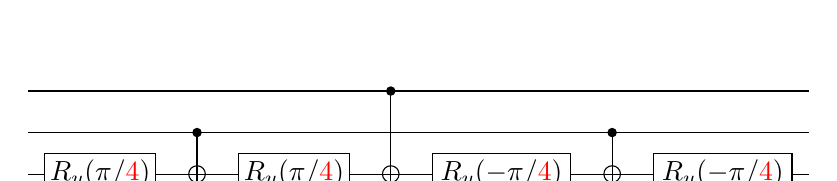
\begin{tikzpicture}[scale=1.000000,x=1pt,y=1pt]
\filldraw[color=white] (0.000000, -7.500000) rectangle (282.000000, 37.500000);
% Drawing wires
% Line 1: a3 W
\draw[color=black] (0.000000,30.000000) -- (282.000000,30.000000);
% Line 2: a2 W
\draw[color=black] (0.000000,15.000000) -- (282.000000,15.000000);
% Line 3: a1 W
\draw[color=black] (0.000000,0.000000) -- (282.000000,0.000000);
% Done with wires; drawing gates
% Line 4: a1 G $R_y(\pi/\textcolor{red}{4})$ width=40 height=15
\begin{scope}
\draw[fill=white] (26.000000, -0.000000) +(-45.000000:28.284271pt and 10.606602pt) -- +(45.000000:28.284271pt and 10.606602pt) -- +(135.000000:28.284271pt and 10.606602pt) -- +(225.000000:28.284271pt and 10.606602pt) -- cycle;
\clip (26.000000, -0.000000) +(-45.000000:28.284271pt and 10.606602pt) -- +(45.000000:28.284271pt and 10.606602pt) -- +(135.000000:28.284271pt and 10.606602pt) -- +(225.000000:28.284271pt and 10.606602pt) -- cycle;
\draw (26.000000, -0.000000) node {$R_y(\pi/\textcolor{red}{4})$};
\end{scope}
% Line 5: +a1 a2
\draw (61.000000,15.000000) -- (61.000000,0.000000);
\begin{scope}
\draw[fill=white] (61.000000, 0.000000) circle(3.000000pt);
\clip (61.000000, 0.000000) circle(3.000000pt);
\draw (58.000000, 0.000000) -- (64.000000, 0.000000);
\draw (61.000000, -3.000000) -- (61.000000, 3.000000);
\end{scope}
\filldraw (61.000000, 15.000000) circle(1.500000pt);
% Line 6: a1 G $R_y(\pi/\textcolor{red}{4})$ width=40 height=15
\begin{scope}
\draw[fill=white] (96.000000, -0.000000) +(-45.000000:28.284271pt and 10.606602pt) -- +(45.000000:28.284271pt and 10.606602pt) -- +(135.000000:28.284271pt and 10.606602pt) -- +(225.000000:28.284271pt and 10.606602pt) -- cycle;
\clip (96.000000, -0.000000) +(-45.000000:28.284271pt and 10.606602pt) -- +(45.000000:28.284271pt and 10.606602pt) -- +(135.000000:28.284271pt and 10.606602pt) -- +(225.000000:28.284271pt and 10.606602pt) -- cycle;
\draw (96.000000, -0.000000) node {$R_y(\pi/\textcolor{red}{4})$};
\end{scope}
% Line 7: +a1 a3
\draw (131.000000,30.000000) -- (131.000000,0.000000);
\begin{scope}
\draw[fill=white] (131.000000, 0.000000) circle(3.000000pt);
\clip (131.000000, 0.000000) circle(3.000000pt);
\draw (128.000000, 0.000000) -- (134.000000, 0.000000);
\draw (131.000000, -3.000000) -- (131.000000, 3.000000);
\end{scope}
\filldraw (131.000000, 30.000000) circle(1.500000pt);
% Line 8: a1 G $R_y(-\pi/\textcolor{red}{4})$ width=50 height=15
\begin{scope}
\draw[fill=white] (171.000000, -0.000000) +(-45.000000:35.355339pt and 10.606602pt) -- +(45.000000:35.355339pt and 10.606602pt) -- +(135.000000:35.355339pt and 10.606602pt) -- +(225.000000:35.355339pt and 10.606602pt) -- cycle;
\clip (171.000000, -0.000000) +(-45.000000:35.355339pt and 10.606602pt) -- +(45.000000:35.355339pt and 10.606602pt) -- +(135.000000:35.355339pt and 10.606602pt) -- +(225.000000:35.355339pt and 10.606602pt) -- cycle;
\draw (171.000000, -0.000000) node {$R_y(-\pi/\textcolor{red}{4})$};
\end{scope}
% Line 9: +a1 a2
\draw (211.000000,15.000000) -- (211.000000,0.000000);
\begin{scope}
\draw[fill=white] (211.000000, 0.000000) circle(3.000000pt);
\clip (211.000000, 0.000000) circle(3.000000pt);
\draw (208.000000, 0.000000) -- (214.000000, 0.000000);
\draw (211.000000, -3.000000) -- (211.000000, 3.000000);
\end{scope}
\filldraw (211.000000, 15.000000) circle(1.500000pt);
% Line 10: a1 G $R_y(-\pi/\textcolor{red}{4})$ width=50 height=15
\begin{scope}
\draw[fill=white] (251.000000, -0.000000) +(-45.000000:35.355339pt and 10.606602pt) -- +(45.000000:35.355339pt and 10.606602pt) -- +(135.000000:35.355339pt and 10.606602pt) -- +(225.000000:35.355339pt and 10.606602pt) -- cycle;
\clip (251.000000, -0.000000) +(-45.000000:35.355339pt and 10.606602pt) -- +(45.000000:35.355339pt and 10.606602pt) -- +(135.000000:35.355339pt and 10.606602pt) -- +(225.000000:35.355339pt and 10.606602pt) -- cycle;
\draw (251.000000, -0.000000) node {$R_y(-\pi/\textcolor{red}{4})$};
\end{scope}
% Done with gates; drawing ending labels
% Done with ending labels; drawing cut lines and comments
% Done with comments
\end{tikzpicture}
\end{center}
\vspace{-5pt}
differs from a Toffoli gate only by relative phases.

    \item p.408. eq (9.49) $\sum_i p_i D(\rho_i, \sigma_i) + D(p_i, q_i)$ should be $\sum_i p_i D(\rho_i, \sigma_i) + \textcolor[rgb]{1,0,0}{2}D(p_i, q_i)$.

    \begin{align*}
    \text{eqn } (9.48) 
        &= \sum_i p_i \Tr (P(\rho_i - \sigma_i)) + \sum_i (p_i - q_i) \Tr (P \sigma_i)\\
        &\leq \sum_i p_i \Tr (P(\rho_i - \sigma_i)) + \sum_i |p_i - q_i| \Tr (P \sigma_i)~~~(\because p_i - q_i \leq |p_i - q_i|)\\
        &\leq \sum_i p_i \Tr (P(\rho_i - \sigma_i)) + \sum_i |p_i - q_i|~~~(\because \Tr (P \sigma_i) \leq 1)\\
        &= \sum_i p_i \Tr (P(\rho_i - \sigma_i)) + 2 \frac{\sum_i |p_i - q_i|}{2}\\
        &= \sum_i p_i \Tr (P(\rho_i - \sigma_i)) + 2D(p_i, q_i)
    \end{align*}
%
    \item p.409. Exercise 9.12. If $\rho = \sigma$, then $D(\rho, \sigma) = 0$. Furthermore trace distance is non-negative. Therefore $0 \leq D(\mathcal{E}(\rho), \mathcal{E}(\sigma)) \leq 0 \Rightarrow D(\mathcal{E}(\rho), \mathcal{E}(\sigma))  = 0$. So I think the map $\mathcal{E}$ is not strictly contractive. If $p \neq 1$ and $\rho \neq \sigma$, then $D(\mathcal{E}(\rho), \mathcal{E}(\sigma)) < D(\rho, \sigma)$ is satisfied.
%
    \item p.411. Exercise 9.16. eqn(9.73) $\Tr (A^\dagger B) = \braket{m | A \otimes B | m}$ should be $\Tr (A^{\textcolor{red}{T}} B) = \braket{m | A \otimes B | m}$.

    Simple counter example is the case that
    $A = \begin{bmatrix}
        i & 0\\
        0 & 0
    \end{bmatrix}$.
    $B = \begin{bmatrix}
        1 & 0\\
        0 & 0
    \end{bmatrix}$,
    In this case,
    \begin{align*}
        A^\dagger B &=
        \begin{bmatrix}
            -i & 0\\
            0 & 0
        \end{bmatrix}
        \begin{bmatrix}
            1 & 0\\
            0 & 0
        \end{bmatrix}
        = \begin{bmatrix}
            -i & 0\\
            0 & 0
        \end{bmatrix},\\
%
        \Tr (A^\dagger B)& = -i,\\
%
        A \otimes B &= \begin{bmatrix}
            i & 0 & 0 & 0\\
            0 & 0 & 0 & 0\\
            0 & 0 & 0 & 0\\
            0 & 0 & 0 & 0
        \end{bmatrix}\\
        \braket{m | A \otimes B | m} &= (\bra{00} + \braket{11}) (A \otimes B) (\ket{00} + \ket{11}) = i.
    \end{align*}
    Thus $\Tr(A^\dagger B) \neq \braket{m | A \otimes B | m}$.

    By using following relation, we can prove.
    \begin{align*}
        (I \otimes A) \ket{m} = (A^T \otimes I) \ket{m}\\
        \Tr (A) = \braket{m | I \otimes A | m}
    \end{align*}
%
    \begin{align*}
        \Tr (A^T B) = \Tr(BA^T) &= \braket{m | I \otimes BA^T |m}\\
            &= \braket{m | (I \otimes B)(I \otimes A^T) |m}\\
            &= \braket{m | (I \otimes B)(A \otimes I) |m}\\ 
            &= \braket{m | A \otimes B | m}.
    \end{align*}

    \item p.515. eqn (11.67) $S(\rho' || \rho)$ should be $S(\rho || \rho \textcolor{red}{'})$.
\end{itemize}


\mainmatter
%!TeX root=../solnQCQI.tex

\chapter{Introduction to quantum mechanics}
\Textbf{2.1} Show that $(1, -1), (1,2)$, and $(2,1)$ are linearly dependent.
\Soln It is enough to express $(0, 0)$ as a linear combination of the specified vectors.
\begin{align*}
	\begin{bmatrix}
		1 \\
		-1
	\end{bmatrix}
	+
	\begin{bmatrix}
		1 \\
		2
	\end{bmatrix}
	-
	\begin{bmatrix}
		2 \\
		1
	\end{bmatrix}
	=
	\begin{bmatrix}
		0 \\
		0
	\end{bmatrix}
\end{align*}

\Textbf{2.2} Suppose $V$ is a vector space with basis vectors $\ket{0}$ and $\ket{1}$, and $A$ is a linear operator
from $V$ to $V$ such that $A\ket{0}=\ket{1}$ and $A\ket{1}=\ket{0}$.  Give a matrix representation for $A$, with
respect to the input bais $\ket{0},\ket{1}$, and the output basis $\ket{0},\ket{1}$.  Find input and output bases which
give rise to a different matrix representation of $A$.
\Soln With specified operations, it is enough to solve for the entries of a 2x2 matrix which
coverts the input vectors expressed as linear combinations of one basis, say $(\ket{a_1},\ket{a_2}),$
into vectors expressed as linear combinations of another basis, say $(\ket{b_1},\ket{b_2})$.
\[
A = \begin{blockarray}{ccc}
\begin{block}{ccc}
& \ket{b_1} & \ket{b_2}\\
    \end{block}
\begin{block}{ c[cc] }
\ket{a_1} & A_{11} & A_{12} \\
\ket{a_2} & A_{21} & A_{22} \\
            \end{block}
        \end{blockarray}
\]
With $(\ket{a_1},\ket{a_2}) = (\ket{0},\ket{1})$ and $(\ket{b_1},\ket{b_2}) = (\ket{0},\ket{1})$, we have
\begin{align*}
	A\ket{0} &:= \ket{1} = 0\ket{0}+1\ket{1}= A_{11}\ket{b_1} + A_{21}\ket{b_2} = A_{11}\ket{0} + A_{21}\ket{1}\Rightarrow A_{11} = 0,\ A_{21} = 1\\
	A\ket{1} &:= \ket{0} = 1\ket{0}+0\ket{1}=A_{12}\ket{b_1} + A_{22}\ket{b_2} = A_{12}\ket{0} + A_{22}\ket{1}\Rightarrow A_{12} = 1,\ A_{22} = 0\\
%
	\therefore A &=
	\begin{bmatrix}
		0 & 1 \\
		1 & 0
	\end{bmatrix}
\end{align*}
If the output basis was $(\ket{b_1},\ket{b_2}) = (\ket{1},\ket{0})$ instead, then $A=I$.  More formally:
\begin{align*}
    A\ket{0} &:= \ket{1} = 1\ket{1}+0\ket{0}= A_{11}\ket{b_1} + A_{21}\ket{b_2} = A_{11}\ket{1} + A_{21}\ket{0}\Rightarrow A_{11} = 1,\ A_{21} = 0\\
    A\ket{1} &:= \ket{0} = 0\ket{1}+1\ket{0}= A_{12}\ket{b_1} + A_{22}\ket{b_2} = A_{12}\ket{1} + A_{22}\ket{0}\Rightarrow A_{12} = 0,\ A_{22} = 1\\
        %
    \therefore A &=
    \begin{bmatrix}
    1 & 0 \\
    0 & 1
    \end{bmatrix}
\end{align*}
With a more interesting orthonormal output basis $(\ket{b_1},\ket{b_2})=(\ket{+},\ket{-})$:
\begin{align*}
        A\ket{0} &:= \ket{1} = \frac{\sqrt{2}}{2}\ket{+}-\frac{\sqrt{2}}{2}\ket{-}= A_{11}\ket{b_1} + A_{21}\ket{b_2} = A_{11}\ket{+} + A_{21}\ket{-}\Rightarrow A_{11} = \frac{\sqrt{2}}{2},\ A_{2} = -\frac{\sqrt{2}}{2}\\
        A\ket{1} &:= \ket{0} = \frac{\sqrt{2}}{2}\ket{+}+\frac{\sqrt{2}}{2}\ket{-}= A_{12}\ket{b_1} + A_{22}\ket{b_2} = A_{12}\ket{+} + A_{22}\ket{-}\Rightarrow A_{12} = \frac{\sqrt{2}}{2},\ A_{22} = \frac{\sqrt{2}}{2}\\
        %
    \therefore A &= \frac{\sqrt{2}}{2}
    \begin{bmatrix}
    1 & -1 \\
    1 & 1
    \end{bmatrix}
\end{align*}
Note: This is similar, but not equal to $\mathbf{H}$.  Had $A$ been the identity transformation when expressed with the
same input and output bases, then the result would have been exactly $\mathbf{H}$.

\Textbf{2.3} Suppose $A$ is a linear operator from vector space $V$  to vector space $W$, and $B$ is a linear operator
from vector space $W$ to vector space $X$.  Let $\ket{v_i}, \ket{w_j},$ and $\ket{x_k}$ be bases for the vector spaces
$V, W,$ and $X$, respectively.  Show that the matrix representation for the linear transformation $BA$ is the matrix
product of the matrix representations for $B$ and $A$ with respect to the appropriate bases.
\Soln Fix $i$.  We'll show that $(B\circ A)_{ki} = (B \cdot A)_{ki}$.
\begin{align*}
(B\circ A) \ket{v_i} = \sum_k (B\circ A)_{ki} \ket{x_k} &= B \left( \sum_{j} A_{ji}\ket{w_j} \right) \tag{Eqn 2.12, composition}\\
	&= \sum_{j} A_{ji} B\ket{w_j}\tag{linearity}\\
	&= \sum_{j,k} A_{ji} B_{kj}\ket{x_k}\tag{Eqn 2.12}\\
	&= \sum_k \left( \sum_j B_{kj} A_{ji}  \right) \ket{x_k}\tag{finiteness, commutativity}\\
    &= \sum_k \left( (B\cdot A)_{ki}  \right) \ket{x_k}\tag{definition}\\\\
	\therefore & (B\circ A)_{ki} = (B\cdot A)_{ki}
\end{align*}



\Textbf{2.4} Show that the identity operator on a vector space $V$ has a matrix representation which is one along the
diagonal and zero everywhere else, if the matrix representation is taken with respect to the same input and output bases.
This matrix is known as the \textit{identity matrix}
\Soln Let $I$ be the matrix in question.
\begin{align*}
I\ket{v_j} := \ket{v_j} &= \sum_i I_{ij} \ket{v_i}, \ \forall j.\\
	&\Rightarrow I_{ij} = \delta_{ij} := \left\{ \begin{array}{cc} 1 & i=j \\ \\ 0 & o/w\end{array}\right.
\end{align*}


\Textbf{2.5} Verify that $(\cdot, \cdot)$ just defined is an inner product on $\mathbb{C}^n$
\Soln Defined inner product on $\mathbb{C}^n$ is
\begin{align*}
	\left(
		(y_1, \cdots, y_n), (z_1, \cdots, z_n)
	\right)
	= \sum_{i} y_i^* z_i .
\end{align*}
Equation (2.13.1), linearity in second argument:
\begin{align*}
	\left((y_1,\cdots,y_n),\sum_i\lambda_i(z_{i1},\cdots,z_{in})\right)
	&= \left((y_1,\cdots,y_n),\left(\sum_i\lambda_iz_{i1},\cdots,\sum_i\lambda_iz_{in}\right)\right) \tag{definition} \\
    &= \sum_jy^*_j\left(\sum_i\lambda_iz_{ij}\right) \tag{definition}\\
    &= \sum_j\left(\sum_iy^*_j\lambda_iz_{ij}\right) \tag{linearity of multiplcation}\\
    &= \sum_j\left(\sum_i\lambda_iy^*_jz_{ij}\right) \tag{associativity/commutativity}\\
    &= \sum_i\left(\sum_j\lambda_iy^*_jz_{ij}\right) \tag{finiteness} \\
    &= \sum_i\lambda_i\left(\sum_jy^*_jz_{ij}\right) \tag{linearity} \\
    &= \sum_i\lambda_i\left((y_1,\cdots,y_n),(z_{i1},\cdots,z_{in})\right) \tag{definition}
\end{align*}
%
%
%    &= \sum_i\lambda_i\left(
%(y_1, \cdots, y_n),(z_{i1}, \cdots, z_{in})
%\right) \tag{definition}
%

% =\sum_i y_i^* \left(
% 										\sum_j \lambda_j z_{ji}
% 			      				   \right)\\
% 	&= \sum_{i,j} y_i^* \lambda_j z_{ji}\\
% 	&= \sum_j \lambda_j \left(\sum_i y_i^* z_{ji}  \right)\\
% 	&= \sum_j \lambda_j \left(
% 													(y_1, \cdots, y_n),  (z_{j1}, \cdots, z_{jn})
% 											  \right)\\
% 	&= \sum_i \lambda_i \left(
% 													(y_1, \cdots, y_n),  (z_{i1}, \cdots, z_{in})
% 												\right).

Equation (2.13.2), conjugate symmetry:
\begin{align}
	\bigl((y_1, \cdots, y_n), (z_1, \cdots, z_n)\bigr)^*
	&= \left(\sum_i y_i^* z_i \right)^* \tag{definition}\\
	&= \left(\sum_i y_i  z_i^* \right) \tag{conjugate symmetry in $\mathbb{C}^1$}\\
	&= \left(\sum_i z_i^* y_i \right) \tag{commutativity in $\mathbb{C}^1$}\\
	&= \bigl((z_1, \cdots, z_n) , (y_1, \cdots, y_n)\bigr) \tag{definition}
\end{align}


Equation (2.13.3), positive definiteness:
\begin{align*}
	\bigl((y_1, \cdots, y_n), (y_1, \cdots, y_n)\bigr)
	&= \sum_i y_i^* y_i \tag{definition}\\
	&= \sum_i |y_i|^2 \tag{definition} \\
	&\geq 0 \tag{positive definiteness of $|\cdot|^2$ over $\mathbb{C}^1$}
\end{align*}

Now:
\begin{align*}
	\bigl((y_1, \cdots, y_n), (y_1, \cdots, y_n)\bigr) = \sum_i |y_i|^2 &\stackrel{?}{=} 0 \tag{hypothesis}\\ \iff |y_i|^2 &= 0\  \forall i \tag{positivity of $|\cdot|^2$}\\ \iff \ y_i\ \  &= 0\  \forall i \tag{positive definiteness of $|\cdot|^2$ over $\mathbb{C}^1$}\\ \iff (y_1, \cdots, y_n) &=  \textbf{0} \tag{definition}
\end{align*}

%Since $|y_i|^2 \geq 0$ for all $i$. Thus
%$\sum_i |y_i|^2 =
%\left(
%	(y_1, \cdots, y_n), (y_1, \cdots, y_n)
%\right) \geq 0
%$.
%
%From now on,  I will show the following statement,
%\begin{align*}
%	\left(
%		(y_1, \cdots, y_n), (y_1, \cdots, y_n)
%	\right) = 0
%	\text{ iff }  (y_1, \cdots, y_n) = 0.
%\end{align*}
%($\Leftarrow$) This is obvious.\\
%($\Rightarrow$)
%Suppose $\left( (y_1, \cdots, y_n), (y_1, \cdots, y_n) \right) = 0$. Then $\sum_i |y_i|^2 = 0$.
%
%Since $|y_i|^2 \geq 0$ for all $i$, if $\sum_i |y_i|^2 = 0$, then $|y_i|^2 = 0$ for all $i$.
%Therefore $|y_i|^2 = 0 \Leftrightarrow y_i = 0$  for all $i$.
%Thus,
%\begin{align*}
%	(y_1, \cdots, y_n) = 0.
%\end{align*}

\Textbf{2.6} Show that any inner product $(\cdot,\cdot)$ is conjugate-linear in the first argument,
\[
\left(\sum_i \lambda_i\ket{w_i}, \ket{v}\right) = \sum_i \lambda_i^{*}(\ket{w_i}, \ket{v}).
\]
\Soln
\begin{align*}
	\left(\sum_i \lambda_i \ket{w_i},\ket{v}\right) &=
	\bigl(\ket{v},\sum_i \lambda_i \ket{w_i}\bigr)^* \tag{conjugate symmetry}\\
	&= \left(\sum_i \lambda_i \bigl(\ket{v},\ket{w_i}  \bigr) \right)^*\tag{linearlity in the 2nd arg.}\\
	&= \sum_i \lambda_i^* \bigl(\ket{v},\ket{w_i} \bigr)^* \tag{distributivity of complex conjugate}\\
	&= \sum_i \lambda_i^* (\ket{w_i},\ket{v}) \tag{conjugate symmetry}
\end{align*}


\Textbf{2.7} Verify that $\ket{w} = (1,1)$ and $\ket{v} = (1,-1)$ are orthogonal.  What are the normailized forms of these vectors?
\Soln
\begin{align*}
	 (\ket{w}, \ket{v}) &= 	\braket{w | v} \tag{notation} \\
	 &= \begin{bmatrix}
		1^* & 1^*
		\end{bmatrix}
		\begin{bmatrix}
		1 \\
		-1
		\end{bmatrix} \tag{definition}\\
	&= 1^*\cdot1 + 1^*\cdot(-1) \tag{matrix multiplication} \\
	&= 1\cdot1 - 1\cdot1 = 0 \tag{arithmetic}\\
%
	\frac{\ket{w}}{\norm{\ket{w}}} &=
	\frac{\ket{w}}{\sqrt{\braket{w|w}}} = \frac{1}{\sqrt{2}} \begin{bmatrix}
	1 \\
	1
	\end{bmatrix}
	= \ket{+} \\
%
	\frac{\ket{v}}{\norm{\ket{v}}} &=
	\frac{\ket{v}}{\sqrt{\braket{v|v}}} = \frac{1}{\sqrt{2}} \begin{bmatrix}
	1 \\
	-1
	\end{bmatrix}
	=\ket{-}
\end{align*}



\Textbf{2.8} Prove that the Gram-Schmidt procedure produces an orthonormal basis.
\Soln
We prove inductively.  For $d = 1$, the only requirement is that the procecure normalize $\ket{w_d}$, which it does by definition for all $d$.   For $d = 2$, suppose $\ket{v_1}, \cdots,\ket{v_{d-1}}$ is a orthonormal basis for the subspace spanned by  $\ket{w_1},\cdots,\ket{w_{d-1}}$.  Being a basis, the subspace spanned by $\ket{v_1},\cdots,\ket{v_{d-1}}$ is the same.  Linear independence of $\ket{w_1},\cdots,\ket{w_d}$ implies that $\ket{w_d}$ is not in this subspace, so $\ket{v_1},\cdots,\ket{v_{d-1}},\ket{w_d}$ is easily seen to be linearly independent as well.  It remains to be shown that $\ket{v_d}$ is linearly independent of $\ket{v_1},\cdots,\ket{v_{d-1}}$, and is orthogonal to all such vectors.  For independence, note that any dependence relation between $\ket{v_1},\cdots,\ket{v_d}$ immediately induces one between $\ket{v_1},\cdots,\ket{v_{d-1}},\ket{w_d}$, violating their independence.  For orthogonality, let $1\leq j\leq d-1$.  We show $\braket{v_j|v_d} = 0$, completing the proof.

\begin{comment}
\begin{align*}
	\ket{v_2} &= \frac{\ket{w_2} - \braket{v_1 | w_2}\ket{v_1}}{\norm{\ket{w_2} - \braket{v_1 | w_2}\ket{v_1}}}\\
	\braket{v_1 | v_2} &= \bra{v_1} \left(\frac{\ket{w_2} - \braket{v_1 | w_2}\ket{v_1}}{\norm{\ket{w_2} - \braket{v_1 | w_2}\ket{v_1}}}\right)\\
		&= \frac{\braket{v_1 | w_2} - \braket{v_1 | w_2}\braket{v_1 | v_1}}{\norm{\ket{w_2} - \braket{v_1 | w_2}\ket{v_1}}}\\
		&= 0.
\end{align*}
\end{comment}


\begin{align*}
	\braket{v_j | v_d} &= \bra{v_j} \left(\frac{\ket{w_d} - \sum_{i=1}^{d-1}\braket{v_i | w_d}\ket{v_i}}{\norm{\ket{w_d} - \sum_{i=1}^{d-1}\braket{v_i | w_d}\ket{v_i}}}\right) \tag{definition}\\
	&= \frac{\braket{v_j | w_d} - \sum_{i=1}^{d-1}\braket{v_i | w_d}\braket{v_j | v_i}}{\norm{\ket{w_d} - \sum_{i=1}^{d-1}\braket{v_i | w_d}\ket{v_i}}} \tag{linearity in the 2nd argument}\\
	&= \frac{\braket{v_j | w_d} - \sum_{i=1}^{d-1}\braket{v_i | w_d}\delta_{ij}}{\norm{\ket{w_d} - \sum_{i=1}^{d-1}\braket{v_i | w_d}\ket{v_i}}} \tag{orthonormality of $\ket{v_1},\cdots,\ket{v_{d-1}}$}\\
	&= \frac{\braket{v_j | w_d} - \braket{v_j | w_d}}{\norm{\ket{w_d} - \sum_{i=1}^{d-1}\braket{v_i | w_d}\ket{v_i}}} \tag{definition of $\delta_{ij}$}\\
	&= 0 \tag{arithmetic}.
\end{align*}

\Textbf{2.9} \textbf{(Pauli operators and the outer product)} The Pauli matrices can be considered as operators with respect to an orthonormal basis $\ket{0}, \ket{1}$ for a two-dimensional Hilbert space.  Express each of the Pauli operators in the outer product notation.
\begin{align*}
	\sigma_0 &= I \hspace{4.5pt}= \ket{0}\bra{0} + \ket{1}\bra{1}\\
	\sigma_x = \sigma_1 &= X = \ket{1}\bra{0} + \ket{0}\bra{1}\\
	\sigma_y = \sigma_2 &= Y \hspace{1.5pt}=  i\ket{1}\bra{0} - i\ket{0}\bra{1}\\
	\sigma_z = \sigma_3 &= Z \hspace{1.5pt}= \ket{0}\bra{0} - \ket{1}\bra{1}
\end{align*}


\Textbf{2.10} Suppose $\ket{v_i}$ is an orthonormal basis for an inner product space $V$.  What is the matrix representation for the operator $\ket{v_j}\bra{v_k}$, with respect to the $\ket{v_i}$ basis?
\Soln \begin{comment} Let $\ket{v}=\sum_i a_i\ket{v_i}$ be a vector in $V$. 
\begin{align*}
	(\ket{v_j}\bra{v_k})(\ket{v}) = (\ket{v_j}\bra{v_k})\left(\sum_i a_i\ket{v_i}\right) &= \sum_i\braket{v_k|v_i}\ket{v_j} \tag{definition}\\
	&= \sum_i\delta_{ki}\ket{v_j}
\end{align*}
\end{comment}
\begin{align*}
	\ket{v_j}\bra{v_k} &= I_V \ket{v_j} \bra{v_k} I_V \tag{multiply by identity}\\
	&= \left(\sum_p \ket{v_p}\bra{v_p} \right) \ket{v_j}\bra{v_k} \left(\sum_q \ket{v_q}\bra{v_q} \right) \tag{completeness}\\
	&= \sum_{p,q} \ket{v_p} \braket{v_p|v_j}\braket{v_k | v_q} \bra{v_q} \tag{linearity and outer product definition}\\
	&= \sum_{p,q} \delta_{pj} \delta_{kq} \ket{v_p} \bra{v_q} \tag{orthonormality}
\end{align*}
Thus
\begin{align*}
	\left( \ket{v_j}\bra{v_k} \right)_{pq} = \delta_{pj} \delta_{kq} = \left\{\begin{array}{ll}1 & p=j, k=q \\ 0 & o/w\end{array}.\right. 
\end{align*}
That is, $\ket{v_j}\bra{v_k}$ is a square matrix with a 1 in row $j$,  column $k$, and 0s everywhere else.

\Textbf{(Cauchy-Schwartz inequality} A brief expansion from a mathematician: in equation (2.26), other $\ket{i}$-basis vectors appear, but since $\braket{i|v}=\braket{v|i}^*$, $a\cdot a^* = \norm{a} \geq 0$ for all $a\in\mathbb{C}$, and $\braket{\cdot | \cdot}$ is positive definite, all terms but the first constructed in terms of $\ket{w}$ are non-negative and can be removed, leaving the inequality.

\Textbf{2.11} Eigendecomposition of the Pauli matrices: Find the eigenvectors, eigenvalues, and diagonal representations of the Pauli matrices $X, Y$, and $Z$.
\Soln
\begin{align*}
	X = \begin{bmatrix}
	0 & 1 \\
	1 & 0
	\end{bmatrix},\ \det(X-\lambda I) =
	\det \left(\begin{bmatrix}
	-\lambda & 1 \\
	1 & -\lambda
	\end{bmatrix} \right) = \lambda^2-1 = 0 \Rightarrow \lambda = \pm 1
\end{align*}
If $\lambda = 1$,
\begin{align*}
	\begin{bmatrix}
		0 & 1 \\
		1 & 0
	\end{bmatrix}
	\begin{bmatrix}
		c_1 \\
		c_2
	\end{bmatrix} =
	\begin{bmatrix}
	      c_2 \\
	      c_1
	\end{bmatrix} =
	 1
	\begin{bmatrix}
		c_1 \\
		c_2
	\end{bmatrix}
	\Rightarrow c_2 = c_1
\end{align*}
The eigenspace corresponding to $\lambda = 1$ is the set of vectors $\begin{bmatrix}c \\ c\end{bmatrix}$.  The vector $\frac{1}{\sqrt{2}}\begin{bmatrix} 1 \\ 1\end{bmatrix} = \ket{+}$ is such a unit (normalized) vector. 
If $\lambda = -1$,
\begin{align*}
	\begin{bmatrix}
		0 & 1 \\
		1 & 0
	\end{bmatrix}
	\begin{bmatrix}
		c_1 \\
		c_2
	\end{bmatrix} =
	\begin{bmatrix}
	      c_2 \\
	      c_1
	\end{bmatrix} =
	 -1
	\begin{bmatrix}
		c_1 \\
		c_2
	\end{bmatrix}
	\Rightarrow c_2 = -c_1
\end{align*}
The eigenspace corresponding to $\lambda = -1$ is the set of vectors $\begin{bmatrix}c \\ -c\end{bmatrix}$.  The vector $\frac{1}{\sqrt{2}}\begin{bmatrix} 1 \\ -1\end{bmatrix} = \ket{-}$ is such a unit (normalized) vector.  So, a diagonal representation of $X$ (when expressed in terms of the computational basis) is $\bigl(\ket{+}\bra{+}\bigr)-\bigl(\ket{-}\bra{-}\bigr) = \begin{bmatrix}\frac{1}{2} & \frac{1}{2} \\ \frac{1}{2} & \frac{1}{2}\end{bmatrix} - \begin{bmatrix} \frac{1}{2} & \frac{-1}{2} \\ \frac{-1}{2} & \frac{1}{2}\end{bmatrix} \bigl( = X\bigr)$.

\begin{align*}
	Y = \begin{bmatrix}
	0 & -i \\
	i & 0
	\end{bmatrix},\ \det(Y-\lambda I) =
	\det \left(\begin{bmatrix}
	-\lambda & -i \\
	i & -\lambda
	\end{bmatrix} \right) = \lambda^2-(i)(-i)=\lambda^2 - 1 = 0 \Rightarrow \lambda = \pm 1
\end{align*}
If $\lambda = 1$,
\begin{align*}
	\begin{bmatrix}
		0 & -i \\
		i & 0
	\end{bmatrix}
	\begin{bmatrix}
		c_1 \\
		c_2
	\end{bmatrix} =
	\begin{bmatrix}
	      -i\cdot c_2 \\
	      i\cdot c_1
	\end{bmatrix} =
	 1
	\begin{bmatrix}
		c_1 \\
		c_2
	\end{bmatrix}
	\Rightarrow c_2 = i\cdot c_1
\end{align*}
The eigenspace corresponding to $\lambda = 1$ is the set of vectors $\begin{bmatrix}c \\ i\cdot c\end{bmatrix}$.  The vector $\frac{1}{\sqrt{2}}\begin{bmatrix} 1 \\ i\end{bmatrix}\equiv\ket{\psi_{y^+}}$ is such a unit (normalized) vector. 
If $\lambda = -1$,
\begin{align*}
	\begin{bmatrix}
		0 & -i \\
		i & 0
	\end{bmatrix}
	\begin{bmatrix}
		c_1 \\
		c_2
	\end{bmatrix} =
	\begin{bmatrix}
	      -i\cdot c_2 \\
	      i\cdot c_1
	\end{bmatrix} =
	 -1
	\begin{bmatrix}
		c_1 \\
		c_2
	\end{bmatrix}
	\Rightarrow c_2 = -i\cdot c_1
\end{align*}
The eigenspace corresponding to $\lambda = -1$ is the set of vectors $\begin{bmatrix}c \\ -i\cdot c\end{bmatrix}$.  The vector $\frac{1}{\sqrt{2}}\begin{bmatrix} 1 \\ -i\end{bmatrix}\equiv\ket{\psi_{y^-}}$ is such a unit (normalized) vector.  So, a diagonal representation of $Y$ (when expressed in terms of the computational basis) is $\bigl(\ket{\psi_{y^+}}\bra{\psi_{y^+}}\bigr) - \bigl(\ket{\psi_{y^-}}\bra{\psi_{y^-}}\bigr) = \begin{bmatrix}\frac{1}{2} & \frac{-i}{2} \\ \frac{i}{2} & \frac{1}{2}\end{bmatrix} - \begin{bmatrix}\frac{1}{2} & \frac{i}{2} \\ \frac{-i}{2} & \frac{1}{2}\end{bmatrix} \bigl( = Y\bigr)$.

\begin{align*}
	Z = \begin{bmatrix}
	1 & 0 \\
	0 & -1
	\end{bmatrix},\ \det(Z-\lambda I) =
	\det \left(\begin{bmatrix}
	1-\lambda & 0 \\
	0 & -1-\lambda
	\end{bmatrix} \right) = (\lambda+1)(\lambda- 1) = 0 \Rightarrow \lambda = \pm 1
\end{align*}
If $\lambda = 1$,
\begin{align*}
	\begin{bmatrix}
		1 & 0 \\
		0 & -1
	\end{bmatrix}
	\begin{bmatrix}
		c_1 \\
		c_2
	\end{bmatrix} =
	\begin{bmatrix}
	      c_1 \\
	      -c_2
	\end{bmatrix} =
	 1
	\begin{bmatrix}
		c_1 \\
		c_2
	\end{bmatrix}
	\Rightarrow c_2 = -c_2 \Rightarrow c_2 = 0
\end{align*}
The eigenspace corresponding to $\lambda = 1$ is the set of vectors $\begin{bmatrix}c \\ 0\end{bmatrix}$.  The vector $\begin{bmatrix} 1 \\ 0\end{bmatrix}=\ket{0}$ is such a unit (normalized) vector. 
If $\lambda = -1$,
\begin{align*}
	\begin{bmatrix}
		1 & 0 \\
		0 & -1
	\end{bmatrix}
	\begin{bmatrix}
		c_1 \\
		c_2
	\end{bmatrix} =
	\begin{bmatrix}
	      c_1 \\
	      -c_2
	\end{bmatrix} =
	 -1
	\begin{bmatrix}
		c_1 \\
		c_2
	\end{bmatrix}
	\Rightarrow c_1 = -c_1
\end{align*}
The eigenspace corresponding to $\lambda = -1$ is the set of vectors $\begin{bmatrix}0 \\ c\end{bmatrix}$.  The vector $\begin{bmatrix} 0 \\ 1\end{bmatrix}=\ket{1}$ is such a unit (normalized) vector.  So, the computation basis \textit{is} the eigenbasis for $Z$, and a diagonal representation of $Z$ is $\bigl(\ket{0}\bra{0}\bigr) - \bigl(\ket{1}\bra{1}\bigr) = \begin{bmatrix}1 & 0 \\ 0 & 0\end{bmatrix} - \begin{bmatrix}0 & 0 \\ 0 & -1\end{bmatrix} \bigl( = Z\bigr)$.


\Textbf{2.12} Prove that the matrix $\begin{bmatrix}1 & 0 \\ 1 & 1\end{bmatrix} (\equiv A)$ is not diagonalizable.
\Soln
\begin{align*}\det(A-\lambda I) = 
	\det \left(\begin{bmatrix}
	1 & 0 \\
	1 & 1
	\end{bmatrix} - \lambda I \right) = \det \left(\begin{bmatrix}1-\lambda & 0 \\ 1 & 1-\lambda\end{bmatrix}\right)= (1 - \lambda)^2 = 0 \Rightarrow \lambda = 1\ \mathrm{(with\ multiplicity\ 2)}
\end{align*}
All eigenvectors $\begin{bmatrix}c_1\\c_2\end{bmatrix}$ satisfy:
\begin{align*}
	\begin{bmatrix}
		1 & 0 \\
		1 & 1
	\end{bmatrix}
	\begin{bmatrix}
		c_1 \\
		c_2
	\end{bmatrix} =
	\begin{bmatrix}
	      c_1 \\
	      c_1+c_2
	\end{bmatrix} =
	 1
	\begin{bmatrix}
		c_1 \\
		c_2
	\end{bmatrix}
	\Rightarrow c_1 = 0
\end{align*}
So, the eigenspace corresponding to eigenvalue 1 of $A$ is 1-dimensional, with a single unit (normalized) vector $\begin{bmatrix}0 \\ 1\end{bmatrix}=\ket{1}$. The only possible diagonal representation of $A$ would then be $A = \ket{1}\bra{1}$, but this equality does not hold.  We conclude that $A$ has no diagonal representation and is not diagonalizable.

\Textbf{2.13} If $\ket{w}$ and $\ket{v}$ are any two vectors, show that $\bigl(\ket{w}\bra{v}\bigr)^\dagger = \ket{v}\bra{w}$.
\Soln We show that $\ket{v}\bra{w}$ has the defining property of $\bigl(\ket{w}\bra{v}\bigr)^\dagger$, \textit{i.e.} if $\ket{\psi},\ \ket{\phi}$ are arbitrary vectors in $V$, then $\Bigl(\ket{\psi}, \bigl(\ket{w}\bra{v}\bigr)\ket{\phi}\Bigr) = \Bigl(\bigl(\ket{v}\bra{w}\bigr)\ket{\psi}, \ket{\phi}\Bigr)$.  We do so by expanding $\Bigl(\ket{\psi}, \bigl(\ket{w}\bra{v}\bigr)\ket{\phi}\Bigr)^*$ in two different ways. 
\begin{align*}
	\Bigl(\ket{\psi},\ \bigl(\ket{w}\bra{v}\bigr) \ket{\phi}\Bigr)^* &=
	\Bigl(\bigl(\ket{w}\bra{v}\bigr)^\dagger \ket{\psi},\  \ket{\phi}\Bigr)^* \tag{defintion of $^\dagger$}\\
	&= \Bigl(\ket{\phi},\bigl(\ket{w}\bra{v}\bigr)^\dagger \ket{\psi} \Bigr) \tag{conjugate symmetry}
\end{align*}
On the other hand,
\begin{align*}
	\Bigl(\ket{\psi},\bigl(\ket{w}\bra{v}\bigr) \ket{\phi}\Bigr)^*
	&= \bigl(\braket{\psi | w}, \braket{v | \phi}\bigr)^* \tag{associativity of $\bra{\cdot},\ket{\cdot}, \braket{\cdot|\cdot}$, and $\ket{\cdot}\bra{\cdot}$}\\
	&= \bigl(\braket{\phi | v}, \braket{w | \psi}\bigr)^* \tag{conjugate symmetry}\\
	&= \Bigl(\bra{\phi}, \bigl(\ket{v}\bra{w}\bigr)\ket{\psi}\Bigr). \tag{notation}
\end{align*}
Thus
\begin{align*}
	\Bigl(\ket{\phi},\bigl(\ket{w}\bra{v}\bigr)^\dagger \ket{\psi} \Bigr) = \Bigl(\bra{\phi}, \bigl(\ket{v}\bra{w}\bigr)\ket{\psi}\Bigr) \text{ for arbitrary vectors } \ket{\psi},\ \ket{\phi}
\end{align*}
We conclude that $\bigl(\ket{w}\bra{v}\bigr)^\dagger$ and $\ket{v}\bra{w}$ are \underline{the same operator}, so $\bigl(\ket{w}\bra{v}\bigr)^\dagger = \ket{v}\bra{w}$.

\Textbf{2.14} Anti-linearity of the adjoint: Show that the adjoint operation is anti-linear,
\begin{align*}\left(\sum_ia_iA_i\right)^\dagger = \sum_ia_i^*A_i^\dagger\end{align*}
\Soln It is tempting to assume that $\left(\sum_ia_iA_i\right)^\dagger = \sum_i(a_iA_i)^\dagger$, \textit{i.e.} that the $^\dagger$ transformation is additive, but we don't yet know this. It will follow from the fact that $A^\dagger \equiv (A^*)^T$ given after problem 2.15, and that both $^*$ and $^T$ are linear. This itself is not hard to prove by observing that $(A^*)^T$ has the defining propery of $A^\dagger$, making use of the matrix formulation of the inner product.  Without the assumption though, we must be careful to carry around the full sums until additivity (and in-fact full linearity) is known.

\begin{align*}
	\left(\left(\sum_ia_i A_i\right)^\dagger \ket{\phi},\ \ket{\psi} \right)
	&= \left(\ket{\phi},\left(\sum_ia_i A_i\right) \ket{\psi}\right) \tag{definition of $\dagger$}\\
	&= \left(\ket{\phi}, \sum_ia_iA_i\ket{\psi}\right) \tag{distributivity of matrix multiplication}\\
	&= \sum_ia_i \bigl(\ket{\phi},\ A_i \ket{\psi}\bigr) \tag{linearity in the second argument}\\
	&= \sum_ia_i \left(A_i^\dagger \ket{\phi},\ \ket{\psi}\right) \tag{definition of $\dagger$}\\
	&= \sum_i\left(a_i^* A_i^\dagger \ket{\phi},\ \ket{\psi}\right) \tag{conjugate-linearity in the first argument}\\
	&= \left(\left(\sum_ia_i^* A_i^\dagger\right) \ket{\phi},\ \ket{\psi}\right) \tag{distributivity of matrix multiplication}\\
%
	\text{therefore } \left(\sum_ia_i A_i\right)^\dagger &= \sum_ia_i^* A_i^\dagger \tag*{$\square$}
\end{align*}

\Textbf{2.15} Show that $\left(A^\dagger\right)^\dagger = A$.
\Soln We show that $A$ has the defining property of the adjoint of $A^\dagger$. 
\begin{align*}
	\left(\left(A^\dagger\right)^\dagger\ket{\psi},\ \ket{\phi} \right)
	&= \left(\ket{\psi},\ A^\dagger \ket{\phi}\right) \tag*{$\left(\text{definition of } \left(A^\dagger\right)^\dagger\right)$}\\
	&= \left(A^\dagger \ket{\phi},\ \ket{\psi}\right)^* \tag{conjugate symmetry}\\
	&= (\ket{\phi},\ A\ket{\psi})^* \tag{definition of $A^\dagger$}\\
	&= (A\ket{\psi},\ \ket{\phi}) \tag{conjugate symmetry}\\
	\text{therefore } \left(A^\dagger\right)^\dagger &= A \tag*{$\square$}
\end{align*}

\Textbf{2.16} Show that any projector $P$ satisfies the equation $P^2 = P$.
\begin{align*}
	P &= \sum_i \ket{i}\bra{i}. \tag{definition}\\
	P^2 &= \left(\sum_i \ket{i}\bra{i}\right) \left(\sum_j \ket{j}\bra{j}\right) \tag{square definition}\\
	&= \sum_{i,j} \ket{i}\braket{i | j}\bra{j} \tag{distributivity}\\
	&= \sum_{i,j} \ket{i}\bra{j} \delta_{ij} \tag*{$\bigl(\text{evaluate} \braket{i | j}\bigr)$}\\
	&= \sum_i \ket{i}\bra{i}\tag{evaluate sum over $j$}\\
	&= P \tag{definition}
\end{align*}


\Textbf{2.17} Show that a normal matrix is Hermitian if and only if it has real eigenvalues.
\begin{proof}
	($\Rightarrow$) Suppose $A$ is Hermitian. Then $A=A^\dagger$.
	Let $\lambda$ be an eigenvalue of $A$ with unit-eigenvector $\ket{\lambda}$.  We have:
	\begin{align*}
		A \ket{\lambda} &= \lambda \ket{\lambda} \tag{definition} \\
		\braket{\lambda | A | \lambda} &= \lambda \braket{\lambda | \lambda} \tag*{$\bigl(\text{multiply by } \bra{\lambda}\bigr)$}\\
		& = \lambda. \tag{$\lambda$ is a unit-vector}
	\end{align*}
	Now:
	\begin{align*}
		\lambda^*  &= \braket{\lambda | A | \lambda}^* \tag{conjugate}\\
		&= \bigl(\ket{\lambda} , A\ket{\lambda}\bigl)^* \tag{change notation}\\
		&= \bigl(A\ket{\lambda},\lambda\bigr) \tag{conjugate symmetry} \\
		&= \bigl(A^\dagger\ket{\lambda}, \ket{\lambda}\bigr) \tag{hypothesis} \\
		&= \bigl(\ket{\lambda}, A\ket{\lambda}\bigr) \tag{definiton of $^\dagger$} \\
		&= \lambda \tag{from above}
	\end{align*}
	So the eigenvalue $\lambda$ is real, since only real numbers are equal to their conjugates.
	
	\noindent($\Leftarrow$) To prove the converse we make use of the spectral deomposition theorem. It's proof does \textit{not} use the fact that a normal matrix is Hermition if and only if it's eigenvalues are real, so using it here does not make this proof circular.  Suppose the eigenvalues of $A$ are real. From the spectral decomposition theorem there exists a set of eigenvalues $\lambda_i$ and a corresponding orthonormal basis $\ket{\lambda_i}$ such that
	\begin{align}
		A = \sum_i \lambda_i \kb{\lambda_i} \tag{spectral decomposition}
	\end{align}
From this we have:
	\begin{align*}
		A^\dagger &= \left(\sum_i \lambda_i\kb{\lambda_i}\right)^\dagger \tag{apply adjoint}\\
	&= \sum_i\lambda_i^*\bigl(\kb{\lambda_i}\bigr)^\dagger \tag{anti-linearity}\\
	&= \sum_i \lambda_i \kb{\lambda_i} \tag{$\lambda_i$ real, projectors are Hermitian}\\
								&= A \tag{from spectral decomposition}
	\end{align*}
	Thus $A$ is Hermitian.
\end{proof}

\Textbf{2.18} Show that all eigenvalues of a unitary matrix have modulus 1, that is, can be written in the form $e^{i\theta}$ for some real $\theta$.
\Soln
Suppose $\lambda$ is an eigenvalue with corresponding unit-eigenvector $\ket{v}$
\begin{align*}
	1 &= \braket{v | v} \tag{$\ket{v}$ is a unit vector}\\
	&= \braket{v | I | v} \tag{multiply by identity}\\
	&= \braket{v | U^\dagger U  | v} \tag{$U$ is unitary}\\
	&= \bigl(\bra{v}U^\dagger\bigr)\bigl(U\ket{v}\bigr) \tag{associativity of matrix multiplication}\\
	&= \bigl(U\ket{v}\bigr)^\dagger\bigl(U\ket{v}\bigr) \tag{arithmetic properties of $^\dagger$}\\
	&= \bigl(\lambda\ket{v}\bigr)^\dagger\bigl(\lambda\ket{v}\bigr) \tag{$\ket{v}$ is an eigenvector} \\
	&= \lambda^*\lambda\braket{v | v} \tag{re-apply $^\dagger$ and simplify} \\
	&= \norm{\lambda}^2 \tag{definiton of $\norm{\cdot}$, $\ket{v}$ is a unit-vector}
\end{align*}
Now $\norm{\lambda} = 1$, and all complex numbers with modulus 1 are located on the unit-circle in $\mathbb{C}$ and can be expressed as $e^{i\theta}$ for some real $\theta \bigl(\in[0,2\pi)\bigr)$

\Textbf{2.19} Show that the Pauli matrices are Hermitian and unitary
\Soln
It is easy to see that the Pauli matrices are Hermitian (self-adjoint) given the conjugate-transpose formula.  We still must show that their squares are the identity:
\begin{align*}
	X^\dagger X = X^2 = \begin{bmatrix}
		0 & 1 \\
		1 & 0
	\end{bmatrix}
	\begin{bmatrix}
		0 & 1 \\
		1 & 0
	\end{bmatrix}
	= \begin{bmatrix}
		1 & 0 \\
		0 & 1
	\end{bmatrix} = I
\end{align*}

\begin{align*}
	Y^\dagger Y = Y^2 = \begin{bmatrix}
		0 & -i \\
		i & 0
	\end{bmatrix}
	\begin{bmatrix}
		0 & -i \\
		i & 0
	\end{bmatrix}
	= \begin{bmatrix}
		-i^2 & 0 \\
		0 & -i^2
	\end{bmatrix} 
	= \begin{bmatrix}
		1 & 0 \\
		0 & 1
	\end{bmatrix} = I
\end{align*}

\begin{align*}
	Z^\dagger Z = Z^2 = \begin{bmatrix}
		1 & 0 \\
		0 & -1
	\end{bmatrix}
	\begin{bmatrix}
		1 & 0 \\
		0 & -1
	\end{bmatrix}
	= \begin{bmatrix}
		1 & 0 \\
		0 & (-1)^2
	\end{bmatrix}
	= \begin{bmatrix}
		1 & 0 \\
		0 & 1
	\end{bmatrix} = I
\end{align*}

\Textbf{2.20} Suppose $A'$ and $A''$ are matrix representations of an operator $A$ on a vector space $V$ with respect to two different orthonormal bases, $\ket{v_i}$ and $\ket{w_i}$.  Then the elements of $A'$ and $A''$ are $A'_{ij} = \braket{v_i | A | v_j}$ and $A''_{ij} = \braket{w_i | A | w_j}$.  Characterize the relationship between $A'$ and $A''$.
\Soln
\begin{align*}
	U \equiv \sum_i \ket{w_i}\bra{v_i}&,\ \  \ U^\dagger=\sum_j \ket{v_j}\bra{w_j} \tag{construct a unitary operator and its adjoint}\\
	\\
	A_{ij}^{'} &= \braket{v_i | A | v_j} \tag{given} \\
	&= \braket{v_i | UU^\dagger A UU^\dagger | v_j} \tag{$U$ is unitary; $UU^\dagger=I$} \\
	&= \sum_{p,q,r,s} \braket{v_i | w_p} \braket{v_p | v_q} \braket{w_q | A | w_r} \braket{v_r | v_s} \braket{w_s | v_j} \tag{expand $U,U^\dagger$, apply linearity}\\
	&= \sum_{p,q,r,s} \braket{v_i | w_p} \delta_{pq} A_{qr}^{''} \delta_{rs}  \braket{w_s | v_j} \tag{$\ket{v_i}$ is orthonormal, apply given for $A''$}\\
	&= \sum_{p,r}  \braket{v_i | w_p}  \braket{w_r | v_j} A_{pr}^{''} \tag{collect non-zero terms and re-index}
\end{align*}


\Textbf{2.21} Repeat the proof of the spectral decomposition in Box 2.2 for the case when $M$ is Hermitian, simplifying the proof wherever possible.
\\

\noindent\textit{Theorem 2.1} \textbf{(Spectral decomposition)} A \textit{Hermitian} operator $M$ on a vector space $V$ is diagonal with respect to some orthonormal basis for $V$. 
\begin{proof} We induct on the dimension of $V$, as in the boxed proof.  Let $\lambda$ be an eigenvalue of $M$, $P$ be the projector onto the $\lambda$ eigenspace, and $Q$ the projector onto the orthogonal complement.
\begin{align*}
	M &= IMI \tag{trivial}\\
		&= (P+Q) M (P+Q)\tag{definition of $Q$}\\
		&= PMP + QMP + PMQ + QMQ\tag{expand}\\
\end{align*}
Now $PMP = \lambda P$ and $QMP = 0$ as before. To show that $PMQ = 0$ is as easy as substituting $M^\dagger$: 
\begin{align*}
PMQ &= PM^\dagger Q \tag{$M$ is Heritian}\\
&= P(M^{*T}Q) \tag{$^{\dagger}=^{*T}$}\\
&=(QM^*P)^{T} \tag{properties of $^T$}\\
&=((QMP)^*)^T \tag{properties of $^*$}\\
&= 0 \tag{$QMP = 0$}
\end{align*}
Thus $M = PMP + QMQ$.
Next, we prove $QMQ$ is normal.
\begin{align*}
	QMQ (QMQ)^\dagger &= QMQ Q^\dagger M^\dagger Q^\dagger \tag{properties of $^\dagger$, and symmetry}\\
		&= QMQQM^\dagger Q \tag{projectors are Hermitian} \\
		&= QM^\dagger Q QMQ \tag{$M = M^\dagger$}\\
		&=Q^\dagger M^\dagger Q^\dagger QMQ \tag{projectors are Hermitian} \\
		&= (QMQ)^\dagger QMQ  \tag{properties of $^\dagger$, and symmetry}
\end{align*}
Therefore $QMQ$ is normal.
By induction, $QMQ$ is diagonal.  The rest follows Box 2.2 identically.
\end{proof}

\Textbf{2.22} Prove that two eigenvectors of a Hermitian operator with different eigenvalues are necessarily orthogonal
\Soln
Suppose $A$ is a Hermitian operator and $\ket{v_1}, \ket{v_2}$ are eigenvectors of $A$ with eigenvalues $\lambda_1, \lambda_2$, with $\lambda_1\neq\lambda_2$.
Then
\begin{align*}
	\braket{v_1 | A | v_2} = \lambda_2 \braket{v_1 | v_2}. \tag{definition of $v_1$, linearity of $\braket{\cdot |\cdot}$}
\end{align*}

On the other hand,
\begin{align*}
	\braket{v_1 | A | v_2} &= \braket{v_1 | A^\dagger | v_2} \tag{$A$ is Hermitian}\\ 
	&= \braket{v_2 | A | v_1}^* \tag{properties of $^\dagger$, Hermitian $\Rightarrow$ self-transpose} \\
	&= \lambda_1\braket{v_2 | v_1}^* \tag{definition of $v_1$, linearity of $\braket{\cdot |\cdot}$}\\
	&=  \lambda_1\braket{v_1 | v_2} \tag{properties of $^*$}
\end{align*}

Thus
\begin{align*}
	(\lambda_1 - \lambda_2) \braket{v_1 | v_2}  = 0.
\end{align*}
Since $\lambda_1 - \lambda_2 \neq 0$, we must have $\braket{v_1 | v_2}  = 0$, so $v_1$ and $v_2$ are orthogonal.


\Textbf{2.23} Show that the eigenvalues of a projector $P$  are either 0 or 1.
\Soln Suppose $P$ is projector and $\ket{v}$ is an eigenvector of $P$ with eigenvalue $\lambda$.  By exercise 2.16, $P^2 = P$.  We have $P\ket{v} = \lambda \ket{v}$ by hypothesis.  Alternatively,
\begin{align*}
	P \ket{v} &= P^2 \ket{\lambda} \tag{exercise 2.16} \\
 	&= \lambda  P \ket{v} \tag{hypothesis, linearity} \\
	&= \lambda^2 \ket{v} \tag{hypothesis}
\end{align*}
Therefore
\begin{align*}
	\lambda = \lambda^2\\
	\lambda^2-\lambda = 0 \\
	\lambda (\lambda - 1) = 0\\
	\lambda = 0 \text{ or } 1.
\end{align*}


\Textbf{2.24} \textbf{(Hermiticity of positive operators)} Show that a positive operator is necessarily Hermitian.
\Soln Let $A$ be a positive operator, that is, suppose $\braket{v | A | v}$ is real and $\geq 0$ for all $\ket{v}$.  Define $B =\frac{A + A^\dagger}{2}$ and $ C = \frac{A - A^\dagger}{2i}$.  Simple complex arithmetic will show that $A = B+iC$.  $B$ is clearly Hermitian by commutativity of operator addition. $C$ is also Hermitian by linearity of the adjoint, noting that $\left(\frac{1}{2i}\right)^* = -\frac{1}{2i}$.  There are two ways to proceed: one heuristic, and one mathematically rigorous.  We'll start with a heuristic outline of the proof, then provide some mathematically rigorous detail after the fact. 

Let $v$ be a vector and note that it can be proven (below) that $\braket{v | B | v}$ and $\braket{v | C | v}$  are both real numbers.    Now $\braket{v|A|v} = \braket{v|B+iC|v} = \braket{v|B|v} + i\braket{v|C|v}$ by the construction of $B$ and $C$, and the linearity of $\braket{\cdot|\cdot|\cdot}$.  By hypothesis, $\braket{v|A|v}$ is a non-negative real number, so $\braket{v|C|v} = 0$, since both $\braket{v | B | v}$ and $\braket{v | C | v}$  are real.  This will be enough to show that $C=0$ which yields $A=A^\dagger$ by the definition of $C$, that is, $A$ is Hermiitian.

Now, to complete the proof, we need to rigorously show that both $\braket{v | B | v}$ and $\braket{v | C | v}$ are real numbers, and that if $\braket{v|C|v}=0$ for all $\ket{v}$, then $C = 0$. 
Let $W$ be Hermitian, thus normal, and note that by exercise 2.17, $W$ has real eigenvalues, say $\omega_i$.  By the spectral decomposition theorem there is an orthnomal basis, say $\ket{w_i}$, such that $W=\sum_i \omega_i\ket{w_i}\bra{w_i}$.  Let $\ket{v}$ be an arbitrary vector, expressed in the orthonormal $\ket{w_i}$-basis as $\sum_i \alpha_i\ket{w_i}$.
\begin{align*}
	\braket{v | W | v}  &= \left\langle\sum_j\alpha_j\ket{w_j} \Big\lvert  W \Big\rvert \sum_i\alpha_i\ket{w_i}\right\rangle \tag{by construction}\\
		&= \sum_i \sum_j \alpha_i\alpha_j^*\braket{w_j|W|w_i} \tag{(conjugate) linearity of $\braket{\cdot|\cdot|\cdot}$} \\
		&= \sum_i\sum_j \alpha_i\alpha_j^*\left\langle w_j\Big\lvert\sum_k \omega_k\ket{w_k}\bra{w_k}\Big\rvert w_i\right\rangle  \tag{spectral decomposition}\\
		&= \sum_i\sum_j\sum_k\alpha_i\alpha_j^*\omega_k\braket{w_j|w_k}\braket{w_k|w_i} \tag{linearity of $\braket{\cdot|\cdot|\cdot}$} \\
		&= \sum_i\sum_j\sum_k\alpha_i\alpha_j^*\omega_k\delta_{jk}\delta_{ki} \tag{orthonomality of the $\ket{w_i}$  basis}  \\
		&= \sum_k\alpha_k\alpha_k^*\omega_k \tag{collecting non-zero terms}\\
		&= \sum_k\norm{\alpha_k}^2\omega_k \tag{definition of $\norm{\cdot}$}
\end{align*}
The $\omega_k$ are real numbers by exercise 2.17, and the $\norm{\alpha_k}^2$ are real by the definition of $\norm{\cdot}$, so $\braket{v|W|v|}$ is a sum of real number,  and hence also real itself.  Applying this to $B$ and $C$ above completes the first missing part.  To finally complete the proof we'll require Theorem \ref{diagonalzero} below, more generally applicable to linear operators on complex vector spaces, without the assumption of Hermiticity.  The proof follows an MIT 8.05 Quantum Physics II lecture note  by Prof. Barton Zwiebach (\url{https://ocw.mit.edu/courses/physics/8-05-quantum-physics-ii-fall-2013/lecture-notes/MIT8_05F13_Chap_03.pdf})

\begin{prop} \label{fullzero}
	Let $T$ be a linear operator on a complex vector space $V$. If $\braket{u | T | v } = 0$ for all $\ket{u}, \ket{v} \in V$, then $T = 0$.
\end{prop}
\begin{proof}
	Let $\ket{u} = T\ket{v}$. Then $\Bigl\langle T\ket{v} \Big\vert T | v \Bigr\rangle = \Bigl\langle T\ket{v} \Big\vert  T\ket{v} \Bigr\rangle = \norm{T\ket{v}}^2 = 0$, which implies $T\ket{v} = 0$ for all $v$ by property 3 of the inner product (page 65).  $T$ is identically 0, so is the zero operator, \text{i.e.} $T = 0$.
\end{proof}
\begin{thm}\label{diagonalzero}
	Let $T$ be a linear operator on a complex vector space $V$. If $\braket{v | T | v } = 0$ for all $\ket{v} \in V$, then $T = 0$.
\end{thm}
\begin{proof}
Note that the weakened hypothesis doesn't directly apply if $\ket{u} \neq \ket{v}$.  We show that the ``off-diagonal'', distinct vector hypothesis of Proposition \ref{fullzero} can be derived from the weakened ``diagonal'' hypothesis' of this theorem, that is, if $\braket{v | T | v } = 0$ for all $\ket{v}$, then $\braket{u | T | v } = 0$ for all $\ket{u},\ket{v}$. Then apply proposition \ref{fullzero}

Suppose $\ket{u}, \ket{v} \in V$. Then note that by ``foiling'' the $\braket{\cdot|\cdot|\cdot}$'s, we can show a ``polarization'' identity, expressing $\braket{u|T|v}$ as follows
	\begin{align*}
		\frac{1}{4} \Bigl( \bigl\langle u+v|T|u+v\bigr\rangle - \bigl\langle u-v|T|u-v\bigr\rangle + \frac{1}{i}\bigl\langle u+iv|T|u+iv\bigr\rangle -\frac{1}{i} \bigl\langle u-iv|T|u-iv\bigr\rangle \Bigr) = \\
		\frac{1}{4}\Bigl( \bigl(\braket{u|T|u} + \braket{u|T|v} + \braket{v|T|u} + \braket{v|T|v}\bigr) - \bigl(\braket{u|T|u} - \braket{u|T|v} - \braket{v|T|u} + \braket{v|T|v}\bigr) + \dots \\
		  \frac{1}{i}\bigl(\braket{u|T|u}+ i\braket{u|T|v}- i\braket{v|T|u}+ \braket{v|T|v}\bigr) -  \frac{1}{i}\bigl(\braket{u|T|u}- i\braket{u|T|v}+ i\braket{v|T|u} + \braket{v|T|v}\bigr)\Bigr) = \\
		\frac{1}{4}\bigr(0\braket{u|T|u} + 4\braket{u|T|v} + 0 \braket{v|T|u} + 0\braket{v|T|v}\bigl) = \\
		\braket{u|T|v} 
	\end{align*}
	Applying the diagonal hypothesis to $\ket{u+v}, \ket{u-v}, \ket{u+iv}$, and $\ket{u-iv}$ in the first expression above gives that $\braket{u|T|v} = 0$ for all $\ket{u},\ket{v}$, hence by Proposition \ref{fullzero}, $T = 0$.
\end{proof}
Applying Theorem \ref{diagonalzero} to $C$ from above finally completes the proof of the Hermiticity of positive operators.


\Textbf{2.25} Show that for any operator $A$, $A^\dagger A$ is positive.
\Soln Its enough to show that $\braket{v | A^\dagger A|v} \geq 0$ for all $v$, but note that $\braket{v| A^\dagger A|v} = \norm{Av}^2$, which is non-negative, so $A^\dagger A$ is a positive operator.

\Textbf{2.26} Let $\ket{\psi}=(\ket{0}+\ket{1})/\sqrt{2}(=\ket{+})$. Write out $\ket{\psi}^{\otimes2}$ and $\ket{\psi}^{\otimes3}$ explicitly, both in terms of tensor products like $\ket{0},\ket{1}$, and using the Kronecker product.
\Soln
\begin{align*}
	\ket{\psi}^{\otimes 2} &= \frac{1}{\sqrt{2}} (\ket{0} + \ket{1}) \otimes \frac{1}{\sqrt{2}} (\ket{0} + \ket{1}\\
		&= \frac{1}{2} (\ket{00}  + \ket{01} + \ket{10} + \ket{11}  )\\
		&= \frac{1}{2} \begin{bmatrix}
			1 \\
			1 \\
			1 \\
			1
		\end{bmatrix}
\end{align*}

\begin{align*}
	\ket{\psi}^{\otimes 3} &= \frac{1}{\sqrt{2}} (\ket{0} + \ket{1}) \otimes \frac{1}{\sqrt{2}} (\ket{0} + \ket{1}  \otimes \frac{1}{\sqrt{2}} (\ket{0} + \ket{1}\\
		&= \frac{1}{2\sqrt{2}} (\ket{000}  + \ket{001} + \ket{010} + \ket{011} +  \ket{100}  + \ket{101} + \ket{110} + \ket{111})\\
		&= \frac{1}{2\sqrt{2}} \begin{bmatrix}
			1 \\
			1 \\
			1 \\
			1 \\
			1 \\
			1 \\
			1 \\
			1
		\end{bmatrix}
\end{align*}


\Textbf{2.27} Calculate the matrix representations of the tensor products of the Pauli operators (a) $X$ and $Z$; (b) $I$ and $X$; (c) $X$ and $I$. Is the tensor product commutative?

\begin{align*}
	X \otimes Z &= \begin{bmatrix}
		0 & 1 \\
		1 & 0
	\end{bmatrix}
	\otimes
	\begin{bmatrix}
		1 & 0 \\
		0 & -1
	\end{bmatrix} \\
	&= \begin{bmatrix}
		0\begin{bmatrix}
			1 & 0 \\
			0 & -1
			\end{bmatrix}
		&
		1\begin{bmatrix}
			1 & 0 \\
			0 & -1
			\end{bmatrix}
		\\ \\
		1\begin{bmatrix}
			1 & 0 \\
			0 & -1
			\end{bmatrix}
		&
		0\begin{bmatrix}
			1 & 0 \\
			0 & -1
			\end{bmatrix}
	\end{bmatrix} \\
	&= \begin{bmatrix}
		0 & 0 & 1 & 0 \\
		0 & 0 & 0 & -1 \\
		1 & 0 & 0 & 0 \\
		0 & -1 & 0 & 0
	\end{bmatrix}
\end{align*}
\begin{align*}
	I \otimes X &= \begin{bmatrix}
		1 & 0 \\
		0 & 1
	\end{bmatrix}
	\otimes
	\begin{bmatrix}
		0 & 1 \\
		1 & 0
	\end{bmatrix}\\
	&=\begin{bmatrix}
		1\begin{bmatrix}
		0 & 1 \\
		1 & 0
		\end{bmatrix}
		&
		0\begin{bmatrix}
		0 & 1 \\
		1 & 0
		\end{bmatrix}
		\\ \\
		0\begin{bmatrix}
		0 & 1 \\
		1 & 0
		\end{bmatrix}
		&
		1\begin{bmatrix}
		0 & 1 \\
		1 & 0
		\end{bmatrix}
	\end{bmatrix} \\
	&=
	\begin{bmatrix}
	0 & 1 & 0 & 0 \\
	1 & 0 & 0 & 0 \\
	0 & 0 & 0 & 1 \\
	0 & 0 & 1 & 0
	\end{bmatrix}
\end{align*}
\begin{align*}
	X \otimes I &= \begin{bmatrix}
		0 & 1 \\
		1 & 0
	\end{bmatrix}
	\otimes
	\begin{bmatrix}
		1 & 0 \\
		0 & 1
	\end{bmatrix}\\
	&=\begin{bmatrix}
		0\begin{bmatrix}
			1 & 0 \\
			0 & 1
		\end{bmatrix}
		&
		1\begin{bmatrix}
			1 & 0 \\
			0 & 1
		\end{bmatrix}
		\\ \\
		0\begin{bmatrix}
			1 & 0 \\
			0 & 1
		\end{bmatrix}
		&
		1\begin{bmatrix}
			1 & 0 \\
			0 & 1
		\end{bmatrix}
	\end{bmatrix} \\
	&= \begin{bmatrix}
	0 & 0 & 1 & 0 \\
	0 & 0 & 0 & 1 \\
	1 & 0 & 0 & 0 \\
	0 & 1 & 0 & 0
	\end{bmatrix}
\end{align*}

In general, the tensor product is not commutative.

\Textbf{2.28} Show that the transpose, complex conjugation, and adjoint operations distribute over the tensor prodoct,
\begin{align*}(A\otimes B)^* = A^*\otimes B^*; (A\otimes B)^T = A^T\otimes B^T; (A\otimes B)^\dagger = A^\dagger \otimes B^\dagger\end{align*}
\Soln Let $A$ be $n_1\times m_1$ and $B$ be $n_2\times m_2$, so that $A\otimes B$ is $n\times m$, where $n=n_1n_2$ and $m=m_1m_2$.  The entries in $A\otimes B$ are products of a single entry in $A$ and a single entry in $B$.  Specifically, if $i = i_1n_1+i_2$ and $j = j_1m_1+j_2$, with $0\leq i_2 < n_1$ and $0\leq j_2 <  m_1$, then $(A\otimes B)_{ij}= A_{i_1j_1}B_{i_2j_2}$.

\begin{align*}
(A\otimes B)^* &= \left[ A_{i_1j_1}B_{i_2j_2}\right]^* \tag{from above} \\
&= \left[ A_{i_1j_1}^*B_{i_2j_2}^*\right] \tag{piecewise conjugation} \\
&= A^*\otimes B^*\tag{consistent indexing}
\end{align*}
%
%\begin{align*}
%	(A \otimes B)^*
%
%	\begin{comment}
%	\begin{bmatrix}
%		A_{11} B & \cdots & A_{1n} B \\
%		\vdots & \ddots  & \vdots \\
%		A_{m1}B & \cdots & A_{mn} B
%	\end{bmatrix}^* \\
%	&=
%	\begin{bmatrix}
%		A_{11}^* B^* & \cdots & A_{1n}^* B^* \\
%		\vdots & \ddots  & \vdots \\
%		A_{m1}^* B^* & \cdots & A_{mn}^* B^*
%	\end{bmatrix} \\
%	&= A^* \otimes B^*.
%	\end{comment}
%\end{align*}
%
%
%
%	(A\otimes B)^T &= \left[ A_{i_1j_1}B_{i_2j_2}\right]^T \tag{from above} \\
%	&= \left[ A_{j_1i_1}B_{j_2i_2}\right] \tag{definition of $^T$ exchanges $i$ and $j$}
%\end{align*}
To see that $(A\otimes B)^T = A^T\otimes B^T$, note that $A^T\otimes B^T$ is $m\times n$, and $(A^T\otimes B^T)_{kl}$ is the product of a single entry in $A^T$ and a single entry in $B^T$.  Specifically, if $k = k_1m_1+k_2$ and $\ell=\ell_1n_1+\ell_2$, with $0\leq k_2 < m_2$ and $0\leq \ell_2 < n_2$, then $(A^T\otimes B^T)_{k\ell} = (A^T)_{k_1\ell_1}(B^T)_{k_2\ell_2} = A_{\ell_1k_1}B_{\ell_2k_2}$.  Now, the hypotheses on $k$ match the hypotheses on $j$ above, and similarly for $\ell$ and $i$.  This implies $(A^T\otimes B^T)_{k\ell} = (A\otimes B)_{\ell k} = (A\otimes B)^T_{k\ell}$.  All entries in $A^T\otimes B^T$ and $ (A\otimes B)^T$ are equal, so $(A\otimes B)^T = A^T\otimes B^T$.

\begin{comment}
\begin{align*}
	(A\otimes B)^T &=
	\begin{bmatrix}
		A_{11} B & \cdots & A_{1n} B \\
		\vdots & \ddots  & \vdots \\
		A_{m1}B & \cdots & A_{mn} B
	\end{bmatrix}^T \\
	&=
	\begin{bmatrix}
		A_{11} B^T & \cdots & A_{m1} B^T \\
		\vdots & \ddots  & \vdots \\
		A_{1n} B^T & \cdots & A_{mn} B^T
	\end{bmatrix} \\
	&=
	\begin{bmatrix}
		A_{11} B^T & \cdots & A_{1m} B^T \\
		\vdots & \ddots  & \vdots \\
		A_{n1} B^T & \cdots & A_{nm} B^T
	\end{bmatrix} \\
	&= A^T \otimes B^T.
\end{align*}
\end{comment}
Distributivity of $^\dagger$ follows by applying distributivity of $^*$ and $^T$ in turn:
\begin{align*}
	(A\otimes B)^\dagger&=((A \otimes B)^*)^T	\tag{definition of $\dagger$}\\
		&= (A^* \otimes B^*)^T \tag{distribute $^*$}\\
		&= (A^*)^T \otimes (B^*)^T \tag{distribute $^T$}\\
		&= A^\dagger \otimes B^\dagger \tag{definition of $^\dagger$}.
\end{align*}

\Textbf{2.29} Show that the tensor product of two unitary operators is unitary
\Soln
Suppose $U_1$ and $U_2$ are unitary operators. To avoid implicit assumptions on mutliplication of tensor products, let $\ket{v}$ and $\ket{w}$ be vectors in the spaces on which $U_1$ and $U_2$ operate.  Then:
\begin{align*}
	(U_1 \otimes U_2) (U_1 \otimes U_2)^\dagger(\ket{v}\otimes\ket{w}) &= (U_1 \otimes U_2) ( U_1^\dagger \otimes  U_2^\dagger)(\ket{v}\otimes\ket{w})\tag{distributivity of $^\dagger$} \\
	&=(U_1 \otimes U_2)(U_1^\dagger\ket{v}\otimes U_2^\dagger\ket{w}) \tag{definition of tensor product of operators} \\
	&=U_1U_1^\dagger\ket{v}\otimes U_2U_2^\dagger\ket{w} \tag{definition of tensor product of operators} \\
	&= I\ket{v} \otimes I\ket{w} \tag{$U_1$ and $U_2$ are unitary} \\
	&= (I\otimes I)(\ket{v}\otimes\ket{w}) \tag{definition of tensor product of operators} \\
	&= I(\ket{v}\otimes\ket{w}) \tag{$I\otimes I = I$ by construction}
\end{align*}
So, $(U_1\otimes U_2)(U_1\otimes U_2)^\dagger = I$. Similarly, $(U_1 \otimes U_2)^\dagger (U_1 \otimes U_2)  = I \otimes I =  I$, so $U_1\otimes U_2$ is unitary.

\Textbf{2.30} Show that the tensor product of two Hermitian operators is Hermitian.
\Soln
Suppose $A$ and $B$ are Hermitian operators. Then by distributivity of $^\dagger$ and Hermiticity:
\begin{align*}
(A \otimes B)^\dagger = A^\dagger \otimes B^\dagger = A \otimes B.
\end{align*}
Thus $A \otimes B$ is Hermitian.

\Textbf{2.31} Show that the tensor product of two positive operators is positive.
\Soln
Suppose $A$ and $B$ are positive operators.  Then
\begin{align*}
	\Bigl( \ket{\psi} \otimes \ket{\phi} , (A \otimes B) (\ket{\psi} \otimes \ket{\phi})\Bigr) &= \Bigl(\ket{\psi}\otimes\ket{\phi},  A\ket{\psi}\otimes B\ket{\phi}\Bigr) \tag{definition of $A\otimes B$} \\
	&= (\ket{\psi}\otimes\ket{\phi})^\dagger(A\ket{\psi}\otimes B\ket{\phi}) \tag{definition of inner-product}\\
	&=(\bra{\psi}\otimes\bra{\phi})(A\ket{\psi}\otimes B\ket{\phi}) \tag{distributivity of $^\dagger$} \\
	&= \braket{\psi |A| \psi} \braket{\phi | B | \phi}.
\end{align*}
Since $A$ and $B$ are positive operators, $\braket{\psi |A| \psi} \geq 0$ and $\braket{\phi | B | \phi} \geq 0$ for all $\ket{\psi}, \ket{\phi}$, so $\braket{\psi |A| \psi} \braket{\phi | B | \phi} \geq 0$, from which we conclude that $A \otimes B$ is positive.

\Textbf{2.32} Show that the tensor product of two projectors is a projector.
\Soln
Suppose $P_1$ and $P_2$  are projectors. It is tempting to think that by applying exercise 2.16, which yields
\begin{align*}
	(P_1 \otimes P_2) ^2 &= P_1^2 \otimes P_2^2 \tag{tensor product is multiplicative}\\
		&= P_1 \otimes P_2 \tag{exercise 2.16},
\end{align*}
exercise 2.16 would then imply that $ P_1 \otimes P_2$ is also projector. However, this implication is the converse of exercise 2.16, which we have not proven.  Instead, we need to prove that if $P_1 = \sum_{i=0}^k\ket{v_i}\bra{v_i}$ and $P_2=\sum_{j=0}^t\ket{w_j}\bra{w_j}$, where $\ket{v_i}_{i=0}^k$ is a subset of an orthonormal basis $\ket{v_i}_{i=0}^{\kappa}$, and $\ket{w_j}_{j=0}^t$ is a subset of an orthonormal basis $\ket{w_j}_{j=0}^\tau$, then $P_1\otimes P_2 = \sum_{q=0}^s \ket{r_q}\bra{r_q}$, where $\ket{r_q}_{q=0}^{s}$ is a subset of an orthonormal basis $\ket{r_q}_{q=0}^\sigma$.  First, the fact that  $P_1\otimes P_2 = \sum\limits_{\substack{0\leq i\leq k\\0\leq j\leq t}} \bigl(\ket{v_i}\bra{v_i}\bigr)\otimes\bigl(\ket{w_j}\bra{w_j}\bigr)$ follows easily from distributivity of operator tensor products, having illustrated how easily that follows from distributivity of tensor products of vectors in exercise 2.29.  We need to show that $\Bigl\{\bigl(\ket{v_i}\bra{v_i}\bigr)\otimes\bigl(\ket{w_j}\bra{w_j}\bigr)\Bigr\}_{\substack{0\leq i\leq k\\0\leq j\leq t}}$ is a subset of an orthonormal basis.  It is automatically a subset of the set of vector tensor products resulting from loosening the restrictions on $i$ and $j$ to $0\leq i \leq \kappa$ and $0\leq j \leq \tau$, which we may assume is a basis, as stated on page 72.  We need only show that the inner product of tensor products is multiplicative so that orthonormality is preserved.  Let $v_1,v_2,w_1$ and $w_2$ be vectors.
\begin{align*}
\braket{v_1\otimes w_1 | v_2\otimes w_2} &= \ket{v_1\otimes w_1}^\dagger \ket{v_2\otimes w_2} \tag{definition of $\braket{\cdot | \cdot}$}\\
&= \bigl(\ket{v_1}^\dagger\otimes\ket{w_1}^\dagger\bigr)\bigl(\ket{v_2}\otimes\ket{w_2}\bigr) \tag{distributivity of $^\dagger$ over $\otimes$} \\
&= \bigl(\ket{v_1}^\dagger\ket{v_2}\bigr)\otimes\bigl(\ket{w_1}^\dagger\ket{w_2}\bigr) \tag{mixed-product property of kronecker product} \\
&= \braket{v_1|v_2}\otimes\braket{w_1|w_2} \tag{definition of $\braket{\cdot|\cdot}$}\\
&= \braket{v_1|v_2}\braket{w_1|w_2} \tag{$\braket{\cdot|\cdot}$ is a scalar}
\end{align*} 
So, in the basis $\Bigl\{\bigl(\ket{v_i}\bra{v_i}\bigr)\otimes\bigl(\ket{w_j}\bra{w_j}\bigr)\Bigr\}_{\substack{0\leq i\leq \kappa\\0\leq j\leq \tau}}$, the inner product of two vectors $\ket{v_{i_1}}\otimes\ket{w_{j_1}}$ and $\ket{v_{i_2}}\otimes\ket{w_{j_2}}$ is $\braket{v_{i_1}\otimes w_{j_1} | v_{i_2}\otimes w_{j_2}} = \braket{v_{i_1}|v_{i_2}}\braket{w_{j_1}|w_{j_2}}=\delta_{i_1i_2}\delta_{j_1j_2}$, from which it follows that this basis is orthonormal, completing the proof.

\Textbf{2.33} The Hadamard operator on one qubit may be written as $$H=\frac{1}{\sqrt{2}}\Bigl[\bigl(\ket{0}+\ket{1}\bigr)\bra{0}+\bigl(\ket{0}-\ket{1}\bigr)\bra{1}\Bigr].$$  Show explicitly that the Hadamard transform on $n$ qubits, $H^{\otimes n}$, may be written as $$H^{\otimes n} = \frac{1}{\sqrt{2^n}}\sum_{x,y}(-1)^{x\cdot y}\ket{x}\bra{y}.$$ Write out an explicit matrix representation for $H^{\otimes 2}$.
\Soln It is important to note what is meant by $x\cdot y$ in this formula.  Here $\cdot$ does \textbf{not} mean integer multiplcation.  It can be taken to mean popparity of the binary AND of $x$ and $y$. Note that this property is multiplcative across dimensions, when 1 is used for even popparity, and -1 for odd.  We proceed by induction on $n$.  Assume the preceeding formula for $n-1$.  We must prove the formula for $n$.
\begin{align*}
H^{\otimes n} &= H\otimes H^{\otimes n-1}\tag{notation} \\
&=\left(\frac{1}{\sqrt{2}}\Bigl[\bigl(\ket{0}+\ket{1}\bigr)\bra{0}+\bigl(\ket{0}-\ket{1}\bigr)\bra{1}\Bigr]\right) \otimes\left(\frac{1}{\sqrt{2^{n-1}}}\sum_{x,y}(-1)^{x\cdot y}\ket{x}\bra{y}\right)\tag{hypothesis} \\
&=\frac{1}{\sqrt{2^n}}\sum_{x,y}(-1)^{x\cdot y}\bigl(\ket{0}\bra{0}+\ket{1}\bra{0}+\ket{0}\bra{1}-\ket{1}\bra{1}\bigr) \otimes \ket{x}\bra{y}\tag{rearrange} \\
&=\frac{1}{\sqrt{2^n}}\sum_{x',y'}(-1)^{x'\cdot y'}\ket{x'}\bra{y'} \tag{multiplicativity of $\cdot$ accross dimensions}
\end{align*}
Now, explcitly  
\begin{align*}
	H  = \frac{1}{\sqrt{2}} \begin{bmatrix}
		1 & 1 \\
		1 & -1
	\end{bmatrix}
\end{align*}
and
\begin{align*}
	H^{\otimes 2}
	=
	\frac{1}{\sqrt{2}} \begin{bmatrix}
	1 & 1 \\
	1 & -1
	\end{bmatrix}
	\otimes
	\frac{1}{\sqrt{2}} \begin{bmatrix}
	1 & 1 \\
	1 & -1
	\end{bmatrix}
	=
	\frac{1}{2}\begin{bmatrix}
		1\begin{bmatrix}1 & 1 \\
	1 & -1
	\end{bmatrix} & \quad1\begin{bmatrix}1 & 1 \\
	1 & -1
	\end{bmatrix} \\
	1\begin{bmatrix}1 & 1 \\
	1 & -1
	\end{bmatrix} &
	-1\begin{bmatrix}1 & 1 \\
	1 & -1
	\end{bmatrix}
	\end{bmatrix} =
	\frac{1}{2} \begin{bmatrix}
		1 & 1 & 1 & 1 \\
		1 & -1 & 1 & -1 \\
		1 & 1 & -1 & -1 \\
		1 & -1 & -1 & 1
	\end{bmatrix}
\end{align*}

\Textbf{2.34} Find the square root and logarithm of the matrix $$\begin{bmatrix}4&3\\3&4\end{bmatrix}.$$
\Soln
Suppose $A = \begin{bmatrix}
4 & 3 \\
3 & 4
\end{bmatrix} $.  We will need the ``spectral'' decompisition $A$.  First, to find the eigenvalues of $A$:
\begin{align*}
	0=\det (A - \lambda I ) &= (4-\lambda)^2 - 3^2\\
		&= \lambda^2 -8\lambda + 7\\
		&= (\lambda - 1)(\lambda - 7)
\end{align*}
So, the eigenvalues of $A$ are $\lambda = 1$, and $\lambda = 7$.  The corresponding eigenvectors can easily be seen to be
$\begin{bmatrix}
	1 \\
	-1
	\end{bmatrix}
$, corresponding to $\lambda=1$, and $\begin{bmatrix}
1 \\
1
\end{bmatrix}
$, coresponding to $\lambda=7$.  To construct an orthonormal basis from these eigenvenctors, we can scale both by $\frac{1}{\sqrt{2}}$, and denote these scaled vectors by $\ket{\lambda=1}=\frac{1}{\sqrt{2}}\begin{bmatrix}
	1 \\
	-1
	\end{bmatrix}$ and $\ket{\lambda=7}=\frac{1}{2}\begin{bmatrix}
	1 \\
	1
	\end{bmatrix}$. Now, seeing as $A$ is real and self-transpose/adjoint, it is a normal matrix/operator, and as such, $A$ can be ``spectrally decomposed''/diagonalized as:
\begin{align*}
	A &= \kb{\lambda = 1} + 7 \kb{\lambda = 7}  \\
	&= \frac{1}{2}\begin{bmatrix}1&-1\\-1&1\end{bmatrix}+7\left(\frac{1}{2}\begin{bmatrix}1&1\\1&1\end{bmatrix}\right).\end{align*}
The square root of $A$ is ``defined'' as:
\begin{align*}
	\sqrt{A} &= \kb{\lambda = 1} + \sqrt{7} \kb{\lambda = 7}\\
		&= \frac{1}{2} \begin{bmatrix}
		1 & -1 \\
		-1 & 1
		\end{bmatrix}
		+
		\frac{\sqrt{7}}{2} \begin{bmatrix}
		1 & 1 \\
		1 & 1
		\end{bmatrix}\\
		&=
		\frac{1}{2}
		 \begin{bmatrix}
			1+\sqrt{7} & -1+\sqrt{7} \\
			-1 + \sqrt{7} & 1+\sqrt{7}
		\end{bmatrix}
\end{align*}
and $log(A)$ is defined as
 \begin{align*}
 	\log (A) &=  \log (1) \kb{\lambda = 1} + \log (7) \kb{\lambda = 7}\\
 		&= \frac{\log (7)}{2} \begin{bmatrix}
	 		1 & 1 \\
	 		1 & 1
 		\end{bmatrix}
 \end{align*}
Note that one would hope that operator functions would respect various properties of the functions, such as inverses. To formally prove such a thing, let us consider the diagonal representation $A=\sum_a a\kb{\lambda=a}$ and the induced definition of $f(A)=\sum_a f(a)\kb{\lambda = a}$.  Note that the $f(a)$ are eigenvalues of $f(A)$, with corresponding eigevectors $\ket{\lambda=a}$, since the fact that the $\ket{\lambda=a}$ are orthonormal gives $\bigl(\sum_a f(a) \kb{\lambda=a}\bigr)\ket{\lambda=a'} = f(a')\ket{\lambda=a'}$.  So $\sum_a f(a)\kb{\lambda = a}$ is a diagonal representation of $f(a)$.  Now $f^-1(f(A)) = f^{-1}\bigl(\sum_a f(a)\kb{\lambda=a}\bigr) = \sum_a f^{-1}(f(a))\kb{\lambda=a} = \sum_a a \kb{\lambda=a} = A$.


\Textbf{2.35} \textbf{(Exponentiaion of Pauli Matrices)} let $\vec{v}$ be any real three-dimensional unit vector and $\theta$ a real number.  Prove that $$\exp (i\theta\vec{v}\cdot\vec{\sigma}) = \cos(\theta)I+i\sin(\theta)\vec{v}\cdot\vec{\sigma},$$ where $\vec{v}\cdot\vec{\sigma} \equiv \sum_{i=1}^3 v_i\sigma_i$.  This exercise is generalized in problem 2.1 on page 117. 
\Soln To find the eignvalues of $\vec{v}\cdot{\vec{\sigma}}$, we first express in matrix form:
\begin{align*}
	\vec{v} \cdot \vec{\sigma} &= \sum_{i=1}^3 v_i \sigma_i (= v_1\sigma_x + v_2\sigma_y + v_3\sigma_z = v_1X+v_2Y+v_3Z) \tag{definition}\\
		&= v_1 \begin{bmatrix}
		0 & 1 \\
		1 & 0
		\end{bmatrix}
		+ v_2 \begin{bmatrix}
		0 & -i \\
		i & 0
		\end{bmatrix}
		+ v_3 \begin{bmatrix}
		1 & 0 \\
		0 & -1
		\end{bmatrix} \tag{substitute}\\
		&= \begin{bmatrix}
		v_3 & v_1 - i v_2 \\
		v_1 + iv_2 & -v_3
		\end{bmatrix} \tag{collect terms} \\
	0=\det (\vec{v} \cdot \vec{\sigma}  - \lambda I) &= (v_3 - \lambda) (-v_3 - \lambda) - (v_1 - iv_2) (v_1 + iv_2) \tag{characteristic equation}\\
			&= \lambda^2 - (v_1^2 + v_2^2  + v_3^2) \tag{expand and collect $v$'s}\\
			&= \lambda^2 - 1 \tag{$v$ is a unit vector}
\end{align*}
Solving yields that the eigenvalues of $\vec{v}\cdot\vec{\sigma}$ are $\lambda = \pm 1$.
Let $\ket{\lambda_{ \pm 1 } }$ be eigenvectors with eigenvalues $\pm  1$.  Since $\vec{v}$ is a real valued vector, it is easily seen that $\vec{v} \cdot \vec{\sigma}$ is Hermitian, and so is diagonalizable, and we may take the $\ket{\lambda_{\pm 1}}$ to be orthonormal by Exercise 2.22.   In particular, this gives
\begin{align*}
	\kb{\lambda_1} + \kb{\lambda_{-1}} &= I \tag{completeness} \\
	 \kb{\lambda_1} - \kb{\lambda_{-1}} &= \vec{v} \cdot \vec{\sigma} \tag{diagonalization}
\end{align*}
Now
\begin{align*}
	\exp \left(i \theta \vec{v} \cdot \vec{\sigma} \right) &=
	e^{i \theta} \kb{\lambda_1}  + e^{-i \theta} \kb{\lambda_{-1}} \tag{definition}\\
	&= (\cos \theta + i \sin \theta) \kb{\lambda_1} + (\cos \theta - i \sin \theta) \kb{\lambda_{-1}} \tag{Euler's formula}\\
	&= \cos \theta (\kb{\lambda_1} + \kb{\lambda_{-1}}) + i \sin \theta (\kb{\lambda_1} - \kb{\lambda_{-1}}) \tag{group $\cos$ and $\sin$ terms}\\
	&= \cos( \theta) I + i \sin (\theta) \vec{v} \cdot \vec{\sigma}. \tag{from above}
\end{align*}

\Textbf{2.36} Show that the Pauli matrices except for $I$ have trace zero.
\Soln
\begin{align*}
	\Tr (\sigma_1) &= \Tr \left(
		\begin{bmatrix}
		0 & 1 \\
		1 & 0
		\end{bmatrix}
	\right) = 0\\
%
	\Tr (\sigma_2) &= \Tr \left(
		\begin{bmatrix}
		0 & -i \\
		i & 0
		\end{bmatrix}
	\right) = 0\\
%
	\Tr (\sigma_3) &= \Tr \left(
	\begin{bmatrix}
		1 & 0 \\
		0 & -1
	\end{bmatrix}
	\right) = 1 -1 = 0\\
\end{align*}

\Textbf{2.37} \textbf{(Cyclic property of the trace)} If $A$ and $B$ are two linear operators show that $$\Tr(AB)=\Tr(BA).$$
\begin{align*}
	\Tr (AB) &= \sum_i \braket{i | AB | i} \tag{using matrix representation of $AB$}\\
		&=\sum_i \braket{i | A I B | i} \tag{insert $I$}\\
		&= \sum_{i,j} \braket{i | A | j}\braket{j | B | i} \tag{completeness: $I=\sum_j\kb{j}$}\\
		&= \sum_{i,j} \braket{j | B | i} \braket{i | A | j} \tag{commutativity in $\mathbb{C}$}\\
		&= \sum_j \braket{j | BA | j} \tag{completeness: $I=\sum_i\kb{i}$}\\
		&= \Tr (BA) \tag{using matrix representation of $BA$}
\end{align*}



\Textbf{2.38} \textbf{(Linearity of the trace)} If $A$ and $B$ are two linear operators, show that $$\Tr(A+B)=\Tr(A)+\Tr(B)$$ and if $z$ is an arbitrary complex number show that $$\Tr(zA) = z\Tr(A).$$
\Soln
\begin{align*}
	\Tr (A + B) &= \sum_i \braket{i | A+B | i}  \tag{using matrix representation of $A+B$}\\
		&= \sum_i (\braket{i|A|i}  + \braket{i | B | i}  ) \tag{llinearity of $\braket{\cdot|\cdot|\cdot}$}\\
		&= \sum_i \braket{i|A|i} + \sum_i \braket{i|B|i} \tag{separate terms}\\
		&= \Tr (A) + \Tr (B) \tag{using matrix representation of $A$ and $B$}.
\end{align*}

\begin{align*}
	\Tr (z A) &=  \sum_i \braket{i | z A | i} \tag{matrix representation}\\
		&= \sum_i z \braket{i | A | i} \tag{linearity}\\
		&= z \sum_i \braket{i | A | i}\tag{linearity of sum}\\
		&= z \Tr (A) \tag{matrix representation}.
\end{align*}

\Textbf{2.39} \textbf{(The Hilbert-Schmidt inner product on operators)} The set $L_V$ of linear operators on a Hilbert space $V$ is a vector space.  An important additional result is that the vector space $L_V$ can be given a natural inner product structure, turning it into a Hilbert space.\newline
(1) Show that the function $(\cdot,\cdot)$ on $L_V\times L_V$ defined by $$(A, B) \equiv \Tr(A^\dagger B)$$ is an inner product function.  This inner product is known as the \textit{Hilbert-Schmidt} or \textit{trace} inner product.\newline
(2) If $V$ has $d$ dimensions, show that $L_V$ has dimension $d^2$.\newline
(3) Find an orthonormal bisis of Hermitian matrices for the Hilbert space $L_V$.
\Soln
(1) We check the three properties of inner products on page 65:\newline
\indent(i) linearity in the second argument:
\begin{align*}
\left(A, \sum_i \lambda_i B_i \right) &= \Tr \left(A^\dagger \left(\sum_i \lambda_i B_i  \right) \right) \tag{definition of $(\cdot,\cdot)$}\\
&= \Tr\left(\sum_i \lambda_i A^\dagger B_i\right) \tag{linearity in $L_V$} \\
&= \sum_i \lambda_i \Tr (A^\dagger B_i) \tag{linearity of $\Tr$ from Execise 2.38} \\
&= \sum_i \lambda_i (A,B_i) \qed\tag{definition of $(\cdot, \cdot)$}
\end{align*}
\indent(ii) conjugate symmetry:
\begin{align*}
	(A, B)^* &= \left( \Tr (A^\dagger B) \right)^* \tag{definition}\\
		&= \left(\sum_{i,j} \braket{ i | A^\dagger | j} \braket{j | B | i}  \right)^* \tag{matrix representation, insert $I$, apply completeness}\\
		&= \sum_{i,j}  \braket{j | B | i}^* \braket{ i | A^\dagger | j}^*\tag{distributitivity and multiplicativity of $^*$, cummutativity in $\mathbb{C}$}\\
		&= \sum_{i,j}  \ket{j}^{\dagger*} B^* \ket{i}^* \ket{i}^{\dagger*} A^{\dagger*} \ket{j}^*\tag{distribute conjugation and make $^\dagger$s explicit}\\
		&= \sum_{i,j}   \ket{j}^{T} B^{\dagger T} \ket{i}^{\dagger T} \ket{i}^{T} A^{T} \ket{j}^{\dagger T} \tag{$^{\dagger*} = ^T$, $^*=^{\dagger T}$}\\
		&= \sum_{i,j}   (\ket{i}^{\dagger}B^{\dagger} \ket{j})^T (\ket{j}^{\dagger} A \ket{i})^T \tag{$^T$ is cyclic} \\
		&= \sum_{i,j}   \braket{i|B^{\dagger} |j} \braket{j | A | i} \tag{definition of $\braket{\cdot|\cdot|\cdot}$, transpose in $\mathbb{C}$} \\
		&= \sum_i \braket{i | B^\dagger A | i} \tag{completeness}\\
		&= \Tr (B^\dagger A) = (B, A) \tag{matrix representation, definiton of $(\cdot, \cdot)$}\\
\end{align*}
\indent(iii) positivity:
\begin{align*}
	(A, A) &= \Tr (A^\dagger A) \tag{definition}\\
		&= \sum_i \braket{ i | A^\dagger A | i } \tag{matrix representation} \\
		&\geq 0 \tag{$A^\dagger$ A is positive by Exercise 2.25}
\end{align*}
\begin{adjustwidth}{\parindent}{} We are left only show that if $(A, A) = 0$, then $A = 0$. Note that $(A, A) = 0$ implies that $\braket{i | A^\dagger A | i} = 0$ for all $i$, where here, the $\ket{i}$ are an orthonormal \textit{basis} with respect to which the matrix representation of $A$ is constructed.  Note that $A\ket{i}$ is the $i$-th column of $A$, as constructed on page 64.  Also $\norm{A\ket{i}}^2 = \braket{i | A^\dagger A| i} = 0$, so the $i$-th column of $A$ is $0$, for all $i$.  This gives that $(A, A) = 0$ iff $A=0$, completing the proof of positivity.\end{adjustwidth}

\noindent(2) To show that $L_V$ has dimension $d^2$, note that the elements of $L_V$ are linear operators from $V$ to $V$ and thus have a  matrix represetation by a $d\times d$ matrix.  The vector space of $d\times d$ matrices over $\mathbb{C}$ is clearly $d^2$-dimensional, seeing as the set of matrices populated with all $0$s except for a single 1, where the position of the 1's ranges over all $d^2$ positions, is clearly linearly independent and spans $L_V$.

\noindent(3)  The obvious choice of matrices discussed above is orthonormal, but it is not Hermitian.  Note that for $d=2$, the Pauli matrices are orthonormal with respect to the Hilbert-Schmidt inner prodct, and are Hermitian.  To find such an orthonormal basis for larger $d$, we rely on a generalization called a ``discrete Weyl system''.  See Example 1.6 on page 11 of the lecture notes titled ``Mathematical Introduction to Quantum Information Processing'', from Professor Michael Wolf of the Technical University of Munich (\url{https://www-m5.ma.tum.de/foswiki/pub/M5/Allgemeines/MA5057_2019S/QIPlecture.pdf}), and a convenient diagram incuded in ``Holevo Capacity of Discrete Weyl Channels'', but Rehman et.al (\url{https://www.nature.com/articles/s41598-018-35777-7}).  Unfortunately, neither of those constructions are Hermitian, but a small tweak can be made so.

First, let $\{\ket{i}\}_{i=0}^{d-1}$ be a set of orthonormal basis vectors for $V$.  Define $\omega = e^{\frac{2\pi i}{d}}$, and for $ 0\leq n, m < d$, $$U_{n,m} := \sum_{k=0}^{d-1}\omega^{kn}\ket{k-m}\bra{k},$$
where the subtraction inside the ket is done mod $d$.  Note that $\ket{i}\bra{j}$ is exactly one of the basis matrices discussed above, populated with 0's except for a 1 in positon $i,j$.  To see that these matrices are Hermitian, we must show that for fixed $n,m$, the entry of $U_{n,m}$ in position $i,j$ is the complex conjugate of the entry in position $j,i$.   To be continued.

%\begin{comment}
%To isolate the entry in position $i,j$, note that column $j$ consists of $\omega^{jn}\ket{j-m}$, with $i$-th entry equal to $\omega^{jm}$ iff $j-m\equiv i \Mod{d}$, otherwise $0$.  If $j-m\equiv i \Mod(d}$, then i-ji.if $j-i \not\equiv m\Mod{d}$, then this entry is 0, since the only non-zero entry in column $j$ is  .  Seeing that $i-j\not\equiv m \Mod{d}$ iff $j-i\not\equiv m \Mod{d}$, we see that the entries are complex conjugates in this case
%\begin{align*}
%U_{\ell,k} &= \sum_{r=0}^{d-1}\omega^{rk}\ket{r+k}\bra{r} \tag{definition}
%\end{align*}
%\begin{comment}

%\begin{bmatrix}
%	0 & 1 \\
%	1 & 0
%\end{bmatrix}
%
%\begin{bmatrix}
%	0 & -i \\
%	i & 0
%\end{bmatrix}
%
%\begin{bmatrix}
%	1 & 0 \\
%	0 & -1
%\end{bmatrix}

\Textbf{2.40}
\begin{align*}
	\left[X, Y \right] &=XY - YX\\
		&= \begin{bmatrix}
		0 & 1 \\
		1 & 0
		\end{bmatrix}
		\begin{bmatrix}
		0 & -i \\
		i & 0
		\end{bmatrix}
		-
		\begin{bmatrix}
		0 & -i \\
		i & 0
		\end{bmatrix}
		\begin{bmatrix}
		0 & 1 \\
		1 & 0
		\end{bmatrix} \\
%
		&=
%
		\begin{bmatrix}
			i & 0 \\
			0 & -i
		\end{bmatrix}
		-
		\begin{bmatrix}
			-i & 0 \\
			0 & i
		\end{bmatrix}\\
%
		&=
%
		\begin{bmatrix}
			2i & 0 \\
			0 & -2i
		\end{bmatrix} \\
%
		&=	2i Z
\end{align*}



\begin{align*}
	\left[Y, Z \right] &= \begin{bmatrix}
		0 & -i \\
		i & 0
	\end{bmatrix}
	\begin{bmatrix}
		1 & 0 \\
		0 & -1
	\end{bmatrix}
	-
	\begin{bmatrix}
		1 & 0 \\
		0 & -1
	\end{bmatrix}
	\begin{bmatrix}
		0 & -i \\
		i & 0
	\end{bmatrix}\\
	&=
	\begin{bmatrix}
		0 & 2i \\
		2i & 0
	\end{bmatrix}\\
	&= 2iX
\end{align*}



\begin{align*}
	\left[Z, X\right] &= \begin{bmatrix}
	1 & 0 \\
	0 & -1
	\end{bmatrix}
	\begin{bmatrix}
	0 & 1 \\
	1 & 0
	\end{bmatrix}
	-
	\begin{bmatrix}
	0 & 1 \\
	1 & 0
	\end{bmatrix}
	\begin{bmatrix}
	1 & 0 \\
	0 & -1
	\end{bmatrix}\\
	&=
	2i \begin{bmatrix}
	0 & -i \\
	i & 0
	\end{bmatrix}\\
	&= 2iY
\end{align*}



\Textbf{2.41}
\begin{align*}
\left\{\sigma_1, \sigma_2 \right\} &=\sigma_1 \sigma_2 + \sigma_2 \sigma_1\\
&= \begin{bmatrix}
0 & 1 \\
1 & 0
\end{bmatrix}
\begin{bmatrix}
0 & -i \\
i & 0
\end{bmatrix}
+
\begin{bmatrix}
0 & -i \\
i & 0
\end{bmatrix}
\begin{bmatrix}
0 & 1 \\
1 & 0
\end{bmatrix} \\
%
&=
%
\begin{bmatrix}
i & 0 \\
0 & -i
\end{bmatrix}
+
\begin{bmatrix}
-i & 0 \\
0 & i
\end{bmatrix}\\
%
&= 0
\end{align*}



\begin{align*}
\left\{\sigma_2, \sigma_3 \right\} &= \begin{bmatrix}
0 & -i \\
i & 0
\end{bmatrix}
\begin{bmatrix}
1 & 0 \\
0 & -1
\end{bmatrix}
+
\begin{bmatrix}
1 & 0 \\
0 & -1
\end{bmatrix}
\begin{bmatrix}
0 & -i \\
i & 0
\end{bmatrix}\\
&=0
\end{align*}



\begin{align*}
\left\{\sigma_3, \sigma_1 \right\} &= \begin{bmatrix}
1 & 0 \\
0 & -1
\end{bmatrix}
\begin{bmatrix}
0 & 1 \\
1 & 0
\end{bmatrix}
+
\begin{bmatrix}
0 & 1 \\
1 & 0
\end{bmatrix}
\begin{bmatrix}
1 & 0 \\
0 & -1
\end{bmatrix}\\
&=0
\end{align*}

\begin{align*}
	\sigma_0^2 &= I^2 = I\\
%
	\sigma_1^2 &= \begin{bmatrix}
	0 & 1 \\
	1 & 0
	\end{bmatrix} ^2 = I\\
%
	\sigma_2^2 &= \begin{bmatrix}
	0 & -i \\
	i & 0
	\end{bmatrix} ^2 = I\\
%
	\sigma_3^2 &= \begin{bmatrix}
	1 & 0 \\
	0 & -1
	\end{bmatrix} ^2 = I
\end{align*}



\Textbf{2.42}
\begin{align*}
	\frac{\left[A, B \right] + \left\{A, B\right\}}{2} = \frac{AB - BA + AB + BA}{2} = AB
\end{align*}



\Textbf{2.43}

From eq (2.75) and eq (2.76), $\left\{\sigma_j,  \sigma_k \right\} = 2 \delta_{jk} I$.
From eq (2.77),
\begin{align*}
	\sigma_j \sigma_k &= \frac{\left[\sigma_j, \sigma_k  \right] + \left\{\sigma_j, \sigma_k \right\}}{2}\\
		&= \frac{2i \sum_{l=1}^{3} \epsilon_{jkl}\sigma_l +  2 \delta_{jk} I}{2}\\
		&= \delta_{jk} I + i \sum_{l=1}^{3} \epsilon_{jkl}\sigma_l
\end{align*}


\Textbf{2.44}

By assumption, $\left[A, B\right] = 0$ and $\left\{A, B\right\} = 0$, then $AB = 0$.
Since $A$ is invertible, multiply by $A^{-1}$ from left, then
\begin{align*}
	A^{-1} AB = 0\\
	IB = 0\\
	B=0.
\end{align*}


\Textbf{2.45}
\begin{align*}
	\left[A, B\right]^\dagger &= (AB -BA)^\dagger\\
		&= B^\dagger A^\dagger - A^\dagger B^\dagger\\
		&= \left[B^\dagger, A^\dagger \right]
\end{align*}



\Textbf{2.46}
\begin{align*}
	\left[A, B\right] &= AB - BA\\
		&= - (BA - AB)\\
		&= -\left[B, A\right]
\end{align*}



\Textbf{2.47}
\begin{align*}
	\left(i \left[A, B\right] \right)^\dagger &= -i \left[A, B\right]^\dagger\\
		&= -i \left[B^\dagger, A^\dagger \right]\\
		&= -i \left[B, A \right]\\
		&= i \left[A, B\right]
\end{align*}



\Textbf{2.48}

(Positive )

 Since $P$ is positive, it is diagonalizable. Then $P = \sum_i \lambda_i \kb{i}$, $(\lambda_i \geq 0)$.
\begin{align*}
	J = \sqrt{P^\dagger P} = \sqrt{P P} = \sqrt{P^2} = \sum_i \sqrt{\lambda_i^2} \kb{i} = \sum_i \lambda_i \kb{i} = P.
\end{align*}
 Therefore polar decomposition of $P$ is $P = UP$ for all $P$.
 Thus $U = I$, then $P = P$.


\vspace{5mm}
(Unitary)

Suppose unitary $U$ is decomposed by $U = WJ$ where $W$ is unitary and $J$ is positive, $J = \sqrt{U^\dagger U}$.
\begin{align*}
	J = \sqrt{U^\dagger U} = \sqrt{I} = I
\end{align*}
Since unitary operators are invertible, $W = UJ^{-1} = UI^{-1} = UI = U$.
Thus polar decomposition of $U$ is $U = U$.


\vspace{5mm}
(Hermitian)

Suppose $H = UJ$.
\begin{align*}
	J = \sqrt{H^\dagger H} = \sqrt{HH} = \sqrt{H^2}.
\end{align*}
Thus $H = U\sqrt{H^2}$.

\begin{screen}
	In general, $H \neq \sqrt{H^2}$.

	From spectral decomposition, $H = \sum_i \lambda_i \kb{i}$, $\lambda_i \in \mathds{R}$.
	\begin{align*}
		 \sqrt{H^2} = \sqrt{ \sum_i \lambda_i^2 \kb{i} }
		 =
 		\sum_i
 			\sqrt{
 				\lambda_i^2
			} \kb{i}
		= \sum_i | \lambda_i | \kb{i} \neq H
	\end{align*}
\end{screen}


\Textbf{2.49}

Normal matrix is diagonalizable, $A = \sum_i \lambda_i \kb{i}$.
\begin{align*}
	J &= \sqrt{A^\dagger A} = \sum_i | \lambda_i | \kb{i}.\\
	U &= \sum_i \kbt{e_i}{i}\\
	A &= UJ = \sum_i |\lambda_i| \kbt{e_i}{i}.
\end{align*}



\Textbf{2.50}

Define
$A = \begin{bmatrix}
1 & 0 \\
1 & 1
\end{bmatrix}$.
%
$A^\dagger A = \begin{bmatrix}
2 & 1 \\
1 & 1
\end{bmatrix}$.

 Characteristic equation of $A^\dagger A$ is $\det(A^\dagger A - \lambda I) = \lambda^2 - 3 \lambda + 1 = 0$.
 Eigenvalues of $A^\dagger A$ are $\lambda_\pm = \frac{3 \pm \sqrt{5}}{2}$
 and associated eigenvectors are $\ket{\lambda_\pm} = \frac{1}{\sqrt{10 \mp 2 \sqrt{5}}} \begin{bmatrix}
 2 \\
 -1 \pm \sqrt{5}
 \end{bmatrix} $.

\begin{align*}
	A^\dagger A = \lambda_+ \kb{\lambda_+} + \lambda_- \kb{\lambda_-}.
\end{align*}

 \begin{align*}
 	J = \sqrt{A^\dagger A} &= \sqrt{\lambda_+} \kb{\lambda_+} + \sqrt{\lambda_-} \kb{\lambda_-}\\
 		&= \sqrt{\frac{3 + \sqrt{5}}{2}} \cdot \frac{5 - \sqrt{5}}{40} \begin{bmatrix}
 		4 & 2\sqrt{5} -2 \\
 		2 \sqrt{5} - 2 & 6 -2\sqrt{5}
 		\end{bmatrix}
 		+
 		\sqrt{\frac{3 - \sqrt{5}}{2}} \cdot \frac{5 + \sqrt{5}}{40} \begin{bmatrix}
 		4 & -2\sqrt{5} -2 \\
 		-2 \sqrt{5} - 2 & 6 +2\sqrt{5}
 		\end{bmatrix}
 \end{align*}


\begin{align*}
	J^{-1} = \frac{1}{ \sqrt{\lambda_+} } \kb{\lambda_+} + \frac{1}{ \sqrt{\lambda_-} } \kb{\lambda_-}.
\end{align*}


\begin{align*}
	U = AJ^{-1}
\end{align*}

I'm tired.




\Textbf{2.51}

\begin{align*}
	H^\dagger H = \left(\frac{1}{\sqrt{2}} \begin{bmatrix}
	1 & 1 \\
	1 & -1
	\end{bmatrix}\right)^\dagger
	\frac{1}{\sqrt{2}} \begin{bmatrix}
	1 & 1 \\
	1 & -1
	\end{bmatrix}
	=
	\frac{1}{\sqrt{2}} \begin{bmatrix}
	1 & 1 \\
	1 & -1
	\end{bmatrix}
	\frac{1}{\sqrt{2}} \begin{bmatrix}
	1 & 1 \\
	1 & -1
	\end{bmatrix}
	=
	\frac{1}{2} \begin{bmatrix}
	2 & 0 \\
	0 & 2
	\end{bmatrix}
	=
	I.
\end{align*}




\Textbf{2.52}

\begin{align*}
	H^\dagger = \left(\frac{1}{\sqrt{2}} \begin{bmatrix}
	1 & 1 \\
	1 & -1
	\end{bmatrix}\right)^\dagger
	=
	\frac{1}{\sqrt{2}} \begin{bmatrix}
	1 & 1 \\
	1 & -1
	\end{bmatrix}
	=
	H.
\end{align*}

Thus
\begin{align*}
	H^2 = I.
\end{align*}



\Textbf{2.53}

\begin{align*}
	\det \left(H - \lambda I\right) &= \left(\frac{1}{\sqrt{2}} - \lambda \right) \left(- \frac{1}{\sqrt{2}} - \lambda \right) - \frac{1}{2}\\
		&= \lambda^2 - \frac{1}{2} - \frac{1}{2}\\
		&= \lambda^2 - 1
\end{align*}

Eigenvalues are $\lambda_\pm = \pm 1$ and associated eigenvectors are $\ket{\lambda_\pm} = \frac{1}{\sqrt{4 \mp 2 \sqrt{2}}} \begin{bmatrix}
1 \\
-1 \pm \sqrt{2}
\end{bmatrix} $.




\Textbf{2.54}

Since $[A, B] = 0$, $A$ and $B$ are simultaneously diagonalize, $A = \sum_i a_i \kb{i}$, $B = \sum_i b_i \kb{i}$.
\begin{align*}
	\exp (A) \exp (B) &= \left(\sum_i \exp (a_i) \kb{i}\right) \left(\sum_i \exp (b_i) \kb{i}\right) \\
		&= \sum_{i,j} \exp (a_i + b_j) \ket{i} \braket{i | j} \bra{j}\\
		&= \sum_{i,j} \exp (a_i + b_j) \kbt{i}{j} \delta_{i, j}\\
		&= \sum_i \exp (a_i +  b_i) \kb{i}\\
		&= \exp (A+B)
\end{align*}


\Textbf{2.55}
\begin{align*}
	H = \sum_E E \kb{E}
\end{align*}

\begin{align*}
	U(t_2 - t_1) U^\dagger (t_2 - t_1) &= \exp \left( - \frac{iH(t_2 - t_1)}{\hbar} \right)  \exp \left(  \frac{iH(t_2 - t_1)}{\hbar} \right)\\
		&= \sum_{E, E'} \left(\exp \left(- \frac{iE(t_2 - t_1)}{\hbar} \right) \kb{E} \right)
										\left(\exp \left(- \frac{iE'(t_2 - t_1)}{\hbar} \right) \kb{E'} \right)\\
		&= \sum_{E, E'} \left(\exp \left(- \frac{i(E-E')(t_2 - t_1)}{\hbar} \right) \kbt{E}{E'} \delta_{E,E'} \right) \\
		&= \sum_E \exp(0) \kb{E}\\
		&= \sum_E \kb{E}\\
		&= I
\end{align*}

Similarly, $U^\dagger (t_2 - t_1) U (t_2 - t_1) = I$.



\Textbf{2.56}

$U = \sum_i \lambda_i \kb{\lambda_i}$~~~ ($|\lambda_i| = 1$).
\begin{align*}
	\log (U) &= \sum_j \log (\lambda_j) \kb{\lambda_j} = \sum_j i \theta_j  \kb{\lambda_j} \text{ where } \theta_j = \arg (\lambda_j)\\
	K &= - i \log(U) = \sum_j \theta_j \kb{\lambda_j}.
\end{align*}

\begin{align*}
	K^\dagger = (-i \log U)^\dagger = \left(\sum_j \theta_j \kb{\lambda_j}\right)^\dagger
	= \sum_j \theta_j^* \kb{\lambda_j} = \sum_j \theta_j \kb{\lambda_j} = K
\end{align*}



\Textbf{2.57}
\begin{align*}
	&\ket{\phi} \equiv \frac{L_l \ket{\psi}}{\sqrt{\braket{\psi |L_l^\dagger L_l | \psi}}}\\
	&\braket{\phi | M_m^\dagger M_m | \phi} = \frac{\braket{\psi | L_l^\dagger M_m^\dagger M_m L_l | \psi}}{\braket{\psi | L_l^\dagger L_l | \psi}} \\
%
	&\frac{M_m \ket{\phi}}{\sqrt{\braket{\phi | M_m^\dagger M_m | \phi}}} =
		\frac{M_m L_l \ket{\psi}}{\sqrt{\braket{\psi |L_l^\dagger L_l | \psi}}}
		\cdot
		\frac{ \sqrt{\braket{\psi | L_l^\dagger L_l | \psi}} }{ \sqrt{\braket{\psi | L_l^\dagger M_m^\dagger M_m L_l | \psi}} }
		=
		\frac{M_m L_l \ket{\psi}}{ \sqrt{\braket{\psi | L_l^\dagger M_m^\dagger M_m L_l | \psi}} }
		=
		\frac{N_{lm} \ket{\psi}}{\sqrt{\braket{\psi |N^\dagger_{lm}  N_{lm}  | \psi}}}
\end{align*}



\Textbf{2.58}
\begin{align*}
	\braket{M} &= \braket{ \psi | M | \psi} = \braket{\psi | m | \psi} = m \braket{\psi | \psi} = m\\
	\braket{M^2} &= \braket{ \psi | M^2 | \psi} = \braket{\psi | m^2 | \psi} = m^2 \braket{\psi | \psi} = m^2\\
	\text{deviation} &= \braket{M^2} - \braket{M}^2 = m^2 - m^2 = 0.
\end{align*}


\Textbf{2.59}
\begin{align*}
	\braket{X} &= \braket{0 | X | 0} = \braket{0 | 1} = 0\\
	\braket{X^2} &= \braket{0 | X^2 | 0} = \braket{0 | X | 1} =\braket{0 | 0} = 1\\
	\text{standard deviation} &= \sqrt{ \braket{X^2} - \braket{X}^2 } = 1
\end{align*}


\Textbf{2.60}
\begin{align*}
    \vec{v} \cdot \vec{\sigma} &= \sum_{i=1}^3 v_i \sigma_i\\
    &= v_1 \begin{bmatrix}
        0 & 1 \\
        1 & 0
    \end{bmatrix}
    + v_2 \begin{bmatrix}
        0 & -i \\
        i & 0
    \end{bmatrix}
    + v_3 \begin{bmatrix}
        1 & 0 \\
        0 & -1
    \end{bmatrix} \\
    &= \begin{bmatrix}
        v_3 & v_1 - i v_2 \\
        v_1 + iv_2 & -v_3
    \end{bmatrix}
\end{align*}

\begin{align*}
    \det (\vec{v} \cdot \vec{\sigma}  - \lambda I) &= (v_3 - \lambda) (-v_3 - \lambda) - (v_1 - iv_2) (v_1 + iv_2)\\
    &= \lambda^2 - (v_1^2 + v_2^2  + v_3^2)\\
    &= \lambda^2 - 1 ~~~ (\because |\vec{v}| = 1)
\end{align*}
Eigenvalues are $\lambda = \pm 1$.


(i) if $\lambda = 1$
\begin{align*}
	\vec{v} \cdot \vec{\sigma}  - \lambda I &= \vec{v} \cdot \vec{\sigma}  - I\\
		&= \begin{bmatrix}
    		v_3 - 1 & v_1 - i v_2 \\
    		v_1 + i v_2 & - v_3 - 1
		\end{bmatrix}
\end{align*}

Normalized eigenvector is $\ket{\lambda_1} = \sqrt{ \frac{1+v_3}{2 }} \begin{bmatrix}
1 \\
\frac{1-v_3}{v_1 - iv_2}
\end{bmatrix} $.

\begin{align*}
	\kb{\lambda_1} &= \frac{1+v_3}{2 } \begin{bmatrix}
		1 \\
		\frac{1-v_3}{v_1 - iv_2}
	\end{bmatrix}
	\begin{bmatrix}
   		1 &
   		\frac{1-v_3}{v_1 + iv_2}
	\end{bmatrix}\\
%
	&=
	 \frac{1+v_3}{2 } \begin{bmatrix}
    	 1 & \frac{v_1 - iv_2}{1 + v_3} \\
    	 \frac{v_1 + iv_2}{1 + v_3} & \frac{1-v_3}{1+v_3}
	 \end{bmatrix} \\
	 &=
	 \frac{1}{2} \begin{bmatrix}
    	 1+v_3 & v_1 - iv_2 \\
    	 v_1 + iv_2 & 1 - v_3
	 \end{bmatrix} \\
	 &=
	  \frac{1}{2} \left( I + \begin{bmatrix}
    	 v_3 & v_1 - iv_2 \\
    	 v_1 + iv_2 & - v_3
	 \end{bmatrix} \right) \\
	 &=
	 \frac{1}{2} (I + \vec{v} \cdot \vec{\sigma} )
\end{align*}



(ii) If $\lambda = -1$.
\begin{align*}
	\vec{v} \cdot \vec{\sigma}  - \lambda I &= \vec{v} \cdot \vec{\sigma}  + I\\
	&= \begin{bmatrix}
		v_3 + 1 & v_1 - i v_2 \\
		v_1 + i v_2 & - v_3 + 1
	\end{bmatrix}
\end{align*}

Normalized eigenvalue is $\ket{\lambda_{-1}} = \sqrt{ \frac{1-v_3}{2 }} \begin{bmatrix}
    1 \\
    - \frac{1+v_3}{v_1 - iv_2}
\end{bmatrix} $.


\begin{align*}
	\kb{\lambda_{-1}} &= \frac{1 - v_3}{2} \begin{bmatrix}
	1 \\
	- \frac{1+v_3}{v_1 - iv_2}
	\end{bmatrix}
	\begin{bmatrix}
		1 & - \frac{1+v_3}{v_1 + iv_2}
	\end{bmatrix}\\
	&=
	\frac{1 - v_3}{2} \begin{bmatrix}
		1 & - \frac{v_1 - iv_2}{1 - v_3} \\
		- \frac{v_1 + iv_2}{1 - v_3} & \frac{1+v_3}{1 - v_3}
	\end{bmatrix} \\
	&=
	\frac{1}{2} \begin{bmatrix}
		1 - v_3 & -(v_1 - iv_2) \\
		- (v_1 + iv_2) & 1 + v_3
	\end{bmatrix} \\
	&=
	\frac{1}{2} \left( I - \begin{bmatrix}
		v_3 & v_1 - iv_2 \\
		(v_1 + iv_2 & - v_3
	\end{bmatrix} \right)\\
	&= \frac{1}{2} (I - \vec{v} \cdot \vec{\sigma} ).
\end{align*}


	While I review my proof, I notice that my proof has a defect.
	The case $(v_1,v_2,v_3) = (0,0,1)$, second component of eigenstate, $\frac{1-v_3}{v_1 - iv_2}$, diverges.
	So I implicitly assume $v_1 - iv_2 \neq 0$. Hence my proof is incomplete.

	Since the exercise doesn't require explicit form of projector, we should prove the problem more abstractly.
	In order to prove, we use the following properties of $\vec{v} \cdot \vec{\sigma}$
	\begin{itemize}
		\item $\vec{v} \cdot \vec{\sigma}$ is Hermitian
		\item $(\vec{v} \cdot \vec{\sigma})^2 = I$ where $\vec{v}$ is a real unit vector.
	\end{itemize}

	We can easily check above conditions.
	\begin{align*}
	(\vec{v} \cdot \vec{\sigma})^\dagger &= (v_1 \sigma_1 + v_2 \sigma_2 + v_3 \sigma_3)^\dagger\\
	&= v_1 \sigma_1^\dagger + v_2 \sigma_2^\dagger + v_3 \sigma_3^\dagger\\
	&= v_1 \sigma_1 + v_2 \sigma_2 + v_3 \sigma_3~~~(\because \text{Pauli matrices are Hermitian.})\\
	&= \vec{v} \cdot \vec{\sigma}
	\end{align*}

	\begin{align*}
	(\vec{v} \cdot \vec{\sigma})^2 &= \sum_{j,k=1}^3 (v_j \sigma_j)  (v_k \sigma_k)\\
	&= \sum_{j,k=1}^3 v_j v_k \sigma_j \sigma_k\\
	&= \sum_{j,k=1}^3 v_j v_k \left(\delta_{jk}I + i \sum_{l=1}^3 \epsilon_{jkl}\sigma_l \right) ~~~(\because \text{eqn}(2.78)~ \text{page} 78)\\
	&= \sum_{j,k=1}^3 v_j v_k \delta_{jk}I  + i \sum_{j,k,l=1}^3 \epsilon_{jkl} v_j v_k \sigma_l\\
	&= \sum_{j=1}^3 v_j^2 I\\
	&= I ~~~\left(\because \sum_j v_j^2 = 1 \right)
	\end{align*}


	\begin{proof}
		Suppose $\ket{\lambda}$ is an eigenstate of $\vec{v} \cdot \vec{\sigma}$ with eigenvalue $\lambda$. Then
		\begin{align*}
		\vec{v} \cdot \vec{\sigma} \ket{\lambda} = \lambda \ket{\lambda}\\
		(\vec{v} \cdot \vec{\sigma})^2 \ket{\lambda} = \lambda^2 \ket{\lambda}
		\end{align*}
		On the other hand $(\vec{v} \cdot \vec{\sigma})^2 = I$,
		\begin{align*}
		(\vec{v} \cdot \vec{\sigma})^2 \ket{\lambda} = I \ket{\lambda} = \ket{\lambda}\\
		\therefore \lambda^2\ket{\lambda} = \ket{\lambda}.
		\end{align*}
		Thus $\lambda^2 = 1 \Rightarrow \lambda = \pm 1$. Therefore $\vec{v} \cdot \vec{\sigma}$ has eigenvalues $\pm 1$.

		Let $\ket{\lambda_1}$ and $\ket{\lambda_{-1}}$ are eigenvectors with eigenvalues $1$ and $-1$, respectively.
		I will prove that $P_\pm = \kb{\lambda_{\pm 1}}$.

		In order to prove above equation, all we have to do is prove following condition. (see Theorem \ref{diagonalzero})
		\begin{screen}
			\begin{align}
				\braket{\psi | (P_\pm - \kb{\lambda_{\pm 1}})| \psi} = 0 \text{ for all } \ket{\psi} \in \mathds{C}^2.
			\end{align}
		\end{screen}

		Since $\vec{v} \cdot \vec{\sigma}$ is Hermitian, $\ket{\lambda_1}$ and $\ket{\lambda_{-1}}$ are orthonormal vector ($\because $ Exercise 2.22).
		Let $\ket{\psi} \in \mathds{C}^2$ be an arbitrary state. $\ket{\psi}$ can be written as
		\begin{align*}
		\ket{\psi} = \alpha \ket{\lambda_1} + \beta \ket{\lambda_{\pm 1}} ~~(|\alpha|^2 + |\beta|^2 = 1, \alpha, \beta \in \mathds{C}).
		\end{align*}

		\begin{align*}
		\braket{\psi | (P_{\pm} - \kb{\lambda_\pm})| \psi}
		%		&= \braket{\psi | \left(\frac{1}{2} (I \pm \vec{v} \cdot \vec{\sigma}) - \kb{\lambda_\pm}\right)| \psi}\\
		&= \braket{\psi | P_\pm | \psi} - \braket{\psi | \lambda_\pm} \braket{\lambda_\pm | \psi}.\\
		\braket{\psi | P_\pm | \psi} &= \braket{\psi | \frac{1}{2}(I \pm \vec{v} \cdot \vec{\sigma}) | \psi}\\
		&= \frac{1}{2} \pm \frac{1}{2} \braket{\psi | \vec{v} \cdot \vec{\sigma})| \psi}\\
		&= \frac{1}{2} \pm \frac{1}{2} (|\alpha|^2 - |\beta|^2)\\
		&= \frac{1}{2} \pm \frac{1}{2} (2|\alpha|^2 - 1) ~~~(\because |\alpha|^2 + |\beta|^2 = 1)\\
		\braket{\psi | \lambda_1} \braket{\lambda_1 | \psi} &= |\alpha|^2\\
		\braket{\psi | \lambda_{-1}} \braket{\lambda_{-1}| \psi} &= |\beta|^2 = 1  - |\alpha|^2
		\end{align*}

		Therefore $\braket{\psi | (P_\pm - \kb{\lambda_{\pm 1}})| \psi} = 0$ for all $\ket{\psi} \in \mathds{C}^2$.
		Thus $P_\pm = \kb{\lambda_{\pm 1}}$.
	\end{proof}

\Textbf{2.61}
\begin{align*}
	\braket{\lambda_1 | 0} \braket{0 | \lambda_1} &= \braket{0 | \lambda_1} \braket{\lambda_1 | 0}\\
		&= \braket{0 | \frac{1}{2} ( I + \vec{v} \cdot \vec{\sigma} ) | 0}\\
		&= \frac{1}{2} (1 + v_3)
\end{align*}

Post-measurement state is
\begin{align*}
	\frac{\ket{\lambda_1} \braket{\lambda_1 | 0}}{ \sqrt{\braket{0 | \lambda_1} \braket{\lambda_1 | 0}} } &= \frac{1}{\sqrt{\frac{1}{2} (1 + v_3)}}
	\cdot \frac{1}{2}
	\begin{bmatrix}
		1 + v_3 \\
		v_1 + iv_2
	\end{bmatrix} \\
		&= \sqrt{ \frac{1}{2}  (1 + v_3) } \begin{bmatrix}
		1 \\
		\frac{v_1 + iv_2}{1+v_3}
		\end{bmatrix} \\
		&=  \sqrt{ \frac{1 + v_3}{2} } \begin{bmatrix}
		1 \\
		\frac{1 - v_3}{v_1 - iv_2}
		\end{bmatrix} \\
		&= \ket{\lambda_1}.
\end{align*}



\Textbf{2.62}

Suppose $M_m$ is a measurement operator.
From the assumption, $E_m = M_m^\dagger M_m = M_m$.

Then
\begin{align*}
    \braket{\psi | E_m | \psi} = \braket{\psi | M_m | \psi} \geq 0.
\end{align*}
for all $\ket{\psi}$.

Since $M_m$ is positive operator, $M_m$ is Hermitian.
Therefore,
\begin{align*}
    E_m = M_m^\dagger M_m = M_m M_m = M_m^2 = M_m.
\end{align*}

Thus the measurement is a projective measurement.



\Textbf{2.63}
\begin{align*}
    M_m^\dagger M_m &= \sqrt{E_m} U_m^\dagger U_m \sqrt{E_m}\\
        &= \sqrt{E_m} I \sqrt{E_m}\\
        &= E_m.
\end{align*}

Since $E_m$ is POVM,  for arbitrary  unitary $U$, $M_m^\dagger M_m$ is POVM.



\Textbf{2.64}
Read following paper:
\begin{itemize}
    \item Lu-Ming Duan, Guang-Can Guo.  Probabilistic cloning and identification of linearly independent quantum states. Phys. Rev. Lett.,80:4999-5002, 1998. arXiv:quant-ph/9804064\\
    \url{https://journals.aps.org/prl/abstract/10.1103/PhysRevLett.80.4999}\\
    \url{https://arxiv.org/abs/quant-ph/9804064}
%
    \item Stephen M. Barnett, Sarah Croke, Quantum state discrimination, arXiv:0810.1970 [quant-ph]\\
    \url{https://arxiv.org/abs/0810.1970}\\
    \url{https://www.osapublishing.org/DirectPDFAccess/67EF4200-CBD2-8E68-1979E37886263936_176580/aop-1-2-238.pdf}
\end{itemize}


\Textbf{2.65}
\begin{align*}
    \ket{+} \equiv \frac{\ket{0} + \ket{1}}{\sqrt{2}}, ~~~ \ket{-} \equiv \frac{\ket{0} - \ket{1}}{\sqrt{2}}
\end{align*}


\Textbf{2.66}
\begin{align*}
     X_1 Z_2 \left(\frac{\ket{00} + \ket{11}}{\sqrt{2}} \right) = \frac{\ket{10} - \ket{01}}{\sqrt{2}}
\end{align*}


\begin{align*}
     \braket{X_1 Z_2} = \left(\frac{\bra{00} + \bra{11}}{\sqrt{2}} \right) X_1 Z_2 \left(\frac{\ket{00} + \ket{11}}{\sqrt{2}} \right)
    = \frac{\bra{00} + \bra{11}}{\sqrt{2}}  \cdot \frac{\ket{10} - \ket{01}}{\sqrt{2}}
    = 0
\end{align*}



\Textbf{2.67}

Suppose $W^\perp$ is the orthogonal complement of $W$. Then $V = W \oplus W^\perp$.
Let $\ket{w_i},\ket{w_j'},\ket{u_j'}$ be orthonormal bases for $W$, $W^\perp$, $\left( \mathrm{image}(U) \right)^\perp$, respectively.

% Define $U'$ as $U'|_W\ket{w_i} = U\ket{w_i} (= \ket{u_i})$ and $U'|_{W^\perp}\ket{w_j'} = \ket{u_j'}$
Define $U': V \rightarrow V$ as $U' = \sum_i \kbt{u_i}{w_i} + \sum_j \kbt{u_j'}{w_j'}$,
where $\ket{u_i} = U \ket{w_i}$.


Now
\begin{align*}
    (U')^\dagger U' &= \left( \sum_{i = 1}^{\dim W} \kbt{w_i}{u_i} + \sum_{j = 1}^{\dim W^\perp} \kbt{w_j'}{u_j'} \right)  \left( \sum_i \kbt{u_i}{w_i} + \sum_j \kbt{u_j'}{w_j'} \right)\\
                    &= \sum_i \kb{w_i} + \sum_j \kb{w_j'} = I
\end{align*}
%
and
%
\begin{align*}
    U' (U')^\dagger &= \left( \sum_i \kbt{u_i}{w_i} + \sum_j \kbt{u_j'}{w_j'} \right) \left( \sum_i \kbt{w_i}{u_i} + \sum_j \kbt{w_j'}{u_j'} \right)\\
                    &= \sum_i \kb{u_i} + \sum_j \kb{u_j'} = I.
\end{align*}
%
Thus $U'$ is an unitary operator.
Moreover, for all $\ket{w} \in W$,
\begin{align*}
    U' \ket{w} &= \left( \sum_i \kbt{u_i}{w_i} + \sum_j \kbt{u_j'}{w_j'} \right) \ket{w}\\
               &= \sum_i \ket{u_i} \braket{w_i | w} + \sum_j \ket{u_j'} \braket{w_j' | w}\\
			   &= \sum_i \ket{u_i} \braket{w_i | w}  ~~~(\because \ket{w_j'} \perp \ket{w})\\
			   &= \sum_i U \ket{w_i} \braket{w_i | w}\\
			   &= U \ket{w}.
\end{align*}
%
Therefore $U'$ is an extension of $U$.


\Textbf{2.68}

$\ket{\psi} = \frac{\ket{00} + \ket{11}}{\sqrt{2}}$.

Suppose $\ket{a} = a_0 \ket{0}  + a_1\ket{1}$ and $\ket{b} = b_0 \ket{0}  + b_1\ket{1}$.
%
\begin{align*}
    \ket{a} \ket{b} = a_0 b_0 \ket{00} + a_0 b_1 \ket{01} + a_1 b_0 \ket{10} + a_1 b_1 \ket{11}.
\end{align*}

If $\ket{\psi} = \ket{a} \ket{b}$, then $a_0 b_0 = 1,~ a_0 b_1=0,~ a_1 b_0 = 0,~ a_1 b_1 = 1$ since $\{\ket{ij}\}$ is an orthonormal basis.

If $a_0 b_1 = 0$, then $a_0 = 0$ or $b_1 = 0$.

When $a_0 = 0$ , this is contradiction to $a_0 b_0 = 1$.
When $b_1 = 0$ , this is contradiction to $a_1 b_1 = 1$.

Thus $\ket{\psi} \neq \ket{a} \ket{b}$.


\Textbf{2.69}
Define Bell states as follows.
\begin{align*}
    \ket{\psi_1} &\equiv \frac{\ket{00} + \ket{11}}{\sqrt{2}} = \frac{1}{\sqrt{2}} \begin{bmatrix}
    1 \\
    0 \\
    0 \\
    1
    \end{bmatrix} \\
    \ket{\psi_2} &\equiv \frac{\ket{00} - \ket{11}}{\sqrt{2}} = \frac{1}{\sqrt{2}} \begin{bmatrix}
    1 \\
    0 \\
    0 \\
    -1
    \end{bmatrix} \\
    \ket{\psi_3} &\equiv \frac{\ket{01} + \ket{10}}{\sqrt{2}} = \frac{1}{\sqrt{2}} \begin{bmatrix}
    0 \\
    1 \\
    1 \\
    0
    \end{bmatrix} \\
    \ket{\psi_4} &\equiv \frac{\ket{01} - \ket{10}}{\sqrt{2}} = \frac{1}{\sqrt{2}} \begin{bmatrix}
    0 \\
    1 \\
    -1 \\
    0
    \end{bmatrix} \\
\end{align*}

First, we prove $\{\ket{\psi_i} \}$ is a linearly independent basis.
\begin{align*}
    &a_1 \ket{\psi_1} + a_2 \ket{\psi_2} + a_3 \ket{\psi_3} + a_4 \ket{\psi_4} = 0\\
    &\therefore \frac{1}{\sqrt{2}} \begin{bmatrix}
        a_1 + a_2 \\
        a_3 + a_4 \\
        a_3 - a_4 \\
        a_1 - a_2
    \end{bmatrix} = 0
\end{align*}
\begin{subnumcases}
 \therefore {}
a_1 + a_2 = 0& \nonumber \\
a_3+ a_4 = 0& \nonumber \\
a_3 - a_4 = 0& \nonumber \\
a_1 - a_2 = 0& \nonumber
\end{subnumcases}
\begin{align*}
    \therefore a_1 = a_2 = a_3 = a_4 = 0
\end{align*}
Thus $\{\ket{\psi_i}\}$ is a linearly independent basis.

Moreover $\norm{\ket{\psi_i}} = 1$ and $\braket{\psi_i | \psi_j} = \delta_{ij}$ for $i,j = 1, 2, 3, 4$.
Therefore $\{\ket{\psi_i}\}$ forms an orthonormal basis.




\Textbf{2.70}

For any Bell states we get $\braket{\psi_i | E \otimes I | \psi_i} = \frac{1}{2} (\braket{0|E|0} + \braket{1|E|1})$.

Suppose Eve measures the qubit Alice sent by measurement operators $M_m$.
The probability that Eve gets result $m$ is $p_i(m) = \braket{\psi_i | M_m^\dagger M_m \otimes I | \psi_i}$.
Since $M ^\dagger_m M_m$ is positive, $p_i(m)$ are same values for all $\ket{\psi_i}$.
Thus Eve can't distinguish Bell states.




\Textbf{2.71}

From spectral decomposition,
\begin{align*}
    \rho &= \sum_i p_i \kb{\psi_i}, ~~ p_i \geq 0, ~~ \sum_i p_i = 1.\\
    \rho^2 &= \sum_{i,j} p_i p_j \ket{i}\braket{i|j}\bra{j}\\
        &= \sum_{i,j} p_i p_j \kbt{i}{j}\delta_{ij}\\
        &= \sum_i p_i^2 \kb{i}
\end{align*}

\begin{align*}
    \Tr (\rho^2) &= \Tr \left(\sum_i p_i^2 \kb{i}\right)
        = \sum_i p_i^2 \Tr(\kb{i})
        = \sum_i p_i^2 \braket{i|i}
        = \sum_i p_i^2
        \leq \sum_i p_i = 1~~~ (\because p_i^2 \leq p_i)
\end{align*}

Suppose $\Tr (\rho^2) = 1$. Then $\sum_i p_i^2 = 1$.
Since $p_i^2 < p_i$ for $0 < p_i < 1$,
only single $p_i$ should be 1 and otherwise have to  vanish.
Therefore $\rho = \kb{\psi_i}$. It is a pure state.

Conversely if $\rho$ is pure, then $\rho = \kb{\psi}$.
\begin{align*}
    \Tr (\rho^2) = \Tr (\ket{\psi}\braket{\psi | \psi} \bra{\psi}) = \Tr (\kb{\psi}) = \braket{\psi | \psi} = 1.
\end{align*}



\Textbf{2.72}

(1) Since density matrix is Hermitian, matrix representation is
$\rho = \begin{bmatrix}
    a & b \\ b^* & d
\end{bmatrix}$,
$a, d \in \mathds{R}$ and $b \in \mathds{C}$ w.r.t. standard basis.
Because $\rho$ is density matrix, $\Tr (\rho) = a+d = 1$.

Define $a = (1+r_3)/2$, $d = (1-r_3)/2$ and $b = (r_1 - ir_2)/2$, $(r_i \in \mathds{R})$.

In this case,
\begin{align*}
    \rho = \begin{bmatrix}
        a & b \\ b^* & d
    \end{bmatrix}
    =
    \frac{1}{2} \begin{bmatrix}
        1+r_3 & r_1 - ir_2 \\
        r_1 + ir_2 & 1 - r_3
    \end{bmatrix}
    =
    \frac{1}{2} (I + \vec{r} \cdot \vec{\sigma}).
\end{align*}
Thus for arbitrary density matrix $\rho$ can be written as $\rho = \frac{1}{2} (I + \vec{r} \cdot \vec{\sigma})$.

Next, we derive the condition that $\rho$ is positive.

If $\rho$ is positive, all eigenvalues of $\rho$ should be non-negative.
\begin{align*}
    \det (\rho - \lambda I) &= (a-  \lambda) (b - \lambda) - |b|^2 = \lambda^2 - (a+d)\lambda + ad - |b^2| = 0\\
    \lambda &= \frac{(a+d) \pm \sqrt{(a+d)^2 - 4 (ad - |b|^2)}}{2}\\
        &= \frac{1 \pm \sqrt{1 - 4 \left(\frac{1 - r_3^2}{4} - \frac{r_1^2 + r_2^2}{4} \right)}}{2}\\
        &= \frac{1 \pm \sqrt{1 - (1 - r_1^2 - r_2^2 - r_3^2)}}{2}\\
        &= \frac{1 \pm \sqrt{|\vec{r}|^2}}{2}\\
        &= \frac{1 \pm |\vec{r}|}{2}
\end{align*}

Since $\rho$ is positive, $\frac{1 - |\vec{r}|}{2} \geq 0 \rightarrow |\vec{r}| \leq 1$.

Therefore an arbitrary density matrix for a mixed state qubit is written as $\rho = \frac{1}{2} (I + \vec{r} \cdot \vec{\sigma})$.

\vspace{5mm}
(2)

$\rho = I / 2 \rightarrow \vec{r}  = 0$. Thus  $\rho = I / 2$ corresponds to the origin of Bloch sphere.

\vspace{5mm}
(3)

\begin{align*}
    \rho^2 &= \frac{1}{2} (I + \vec{r} \cdot \vec{\sigma})~ \frac{1}{2} (I + \vec{r} \cdot \vec{\sigma})\\
        &= \frac{1}{4} \left[ I + 2 \vec{r}\cdot \vec{\sigma} + \sum_{j,k}r_j r_k \left(\delta_{jk} I + i \sum_{l=1}^3 \epsilon_{jkl}\sigma_l \right)  \right]\\
        &= \frac{1}{4} \left(I + 2 \vec{r}\cdot \vec{\sigma} + |\vec{r}|^2 I \right)\\
    \Tr (\rho^2) &= \frac{1}{4} (2 + 2|\vec{r}|^2)
\end{align*}

If $\rho$ is pure, then $\Tr (\rho^2) = 1$.
\begin{align*}
   1 =  \Tr (\rho^2) = \frac{1}{4} (2 + 2|\vec{r}|^2)\\
   \therefore |\vec{r}| = 1.
\end{align*}

Conversely, if $|\vec{r}| = 1$, then $\Tr (\rho^2) = \frac{1}{4} (2 + 2|\vec{r}|^2) = 1$. Therefore $\rho$ is pure.




\Textbf{2.73}
\begin{screen}
    \Textbf{Theorem 2.6}
%
    \begin{align*}
        \rho = \sum_i p_i \kb{\psi_i}
            = \sum_i \kb{\tilde{\psi_i}}
            = \sum_j \kb{\tilde{\varphi}_j}
            = \sum_j q_j \kb{\varphi_j}
                ~~ \Leftrightarrow ~~
            \ket{\tilde{\psi}_i} = \sum_j u_{ij} \ket{\tilde{\varphi}_j}
    \end{align*}
    where $u$ is unitary.

	The-transformation in theorem 2.6, $\ket{\tilde{\psi}_i} = \sum_j u_{ij} \ket{\tilde{\varphi}_j}$, corresponds to
	\begin{align*}
	    \left[ \ket{\tilde{\psi}_1} \cdots \ket{\tilde{\psi}_k} \right] = \Big[ \ket{\tilde{\varphi}_1} \cdots \ket{\tilde{\varphi}_k} \Big] U^T
	\end{align*}
	where $k = \mathrm{rank} (\mathcal{\rho})$.
    \begin{align}
        \sum_i \kb{\tilde{\psi_i}} &= \left[ \ket{\tilde{\psi}_1} \cdots \ket{\tilde{\psi}_k} \right]
            \begin{bmatrix}
                \bra{\tilde{\psi_1}}\\
                \vdots\\
                \bra{\tilde{\psi_k}}
            \end{bmatrix}\\
        &= \Big[ \ket{\tilde{\varphi}_1} \cdots \ket{\tilde{\varphi}_k} \Big] U^T
            U^* \begin{bmatrix}
                    \bra{\tilde{\varphi}_1}\\
                    \vdots\\
                    \bra{\tilde{\varphi}_k}
            \end{bmatrix}\\
        &= \Big[ \ket{\tilde{\varphi}_1} \cdots \ket{\tilde{\varphi}_k} \Big]
             \begin{bmatrix}
                \bra{\tilde{\varphi}_1}\\
                \vdots\\
                \bra{\tilde{\varphi}_k}
            \end{bmatrix}\\
        &= \sum_j \kb{\tilde{\varphi}_j}.
    \end{align}
\end{screen}

From spectral theorem, density matrix $\rho$ is decomposed as $\rho = \sum_{k=1}^{d} \lambda_k \kb{k}$ where $d = \dim \mathcal{H}$.
Without loss of generality, we can assume $p_k > 0$ for $k = 1 \cdots , l$ where $l = \mathrm{rank} (\rho)$ and $p_k = 0$ for $k = l+1, \cdots, d$.
Thus $\rho = \sum_{k=1}^{l} p_k \kb{k} = \sum_{k=1}^{l} \kb{\tilde{k}}$, where $\ket{\tilde{k}} = \sqrt{\lambda_k} \ket{k}$.

Suppose $\ket{\psi_i}$ is a state in support $\rho$. Then
\begin{align*}
	\ket{\psi_i} = \sum_{k=1}^l c_{ik} \ket{k}, ~~ \sum_k |c_{ik}|^2 = 1.
\end{align*}

Define $\displaystyle p_i = \frac{1}{\sum_k \frac{|c_{ik}|^2}{\lambda_k} }$ and $\displaystyle u_{ik} = \frac{\sqrt{p_i} c_{ik}}{\sqrt{\lambda_k}}$.

Now
\begin{align*}
	\sum_k |u_{ik}|^2 = \sum_k \frac{p_i | c_{ik} |^2 }{\lambda_k} = p_i \sum_k \frac{| c_{ik} |^2 }{\lambda_k} = 1.
\end{align*}

Next prepare an unitary operator
\footnote{By Gram-Schmidt procedure construct an orthonormal basis $\{\boldsymbol{u}_j\}$ (row vector) with $\boldsymbol{u}_i = [u_{i1} \cdots u_{ik} \cdots u_{il}]$. Then define unitary $U = \begin{bmatrix}
    \boldsymbol{u}_1 \\
    \vdots \\
    \boldsymbol{u}_i \\
    \vdots \\
    \boldsymbol{u}_l
    \end{bmatrix}$.}
such that $i$th row of $U$ is $[u_{i1} \cdots u_{ik} \cdots u_{il}]$.
Then we can define another ensemble such that
\begin{align*}
	\Big[  \ket{\tilde{\psi}_1} \cdots  \ket{\tilde{\psi}_i} \cdots \ket{\tilde{\psi}_l}\Big] = \Big[ \ket{\tilde{k}_1} \cdots \ket{\tilde{k}_l} \Big] U^T
\end{align*}
where $\ket{\tilde{\psi_i}} = \sqrt{p_i} \ket{\psi_i}$.
From theorem 2.6,
\begin{align*}
	\rho = \sum_k \kb{\tilde{k}} = \sum_k \kb{\tilde{\psi}_k}.
\end{align*}

Therefore we can obtain a minimal ensemble for $\rho$ that contains $\ket{\psi_i}$.

Moreover since $\rho^{-1} = \sum_k \frac{1}{\lambda_k} \kb{k}$,
\begin{align*}
	\braket{\psi_i | \rho^{-1} | \psi_i} = \sum_k \frac{1}{\lambda_k} \braket{\psi_i | k} \hspace{-1mm} \braket{k | \psi_i} = \sum_k \frac{|c_{ik}|^2}{\lambda_k} = \frac{1}{p_i}.
\end{align*}

Hence, $ \frac{1}{\braket{\psi_i | \rho^{-1} | \psi_i}} = p_i $.


\Textbf{2.74}
\begin{align*}
	\rho_{AB} &= \kb{a}_A \otimes \kb{b}_B\\
	\rho_A &= \Tr_{B} \rho_{AB} = \kb{a} \Tr (\kb{b}) = \kb{a}\\
	\Tr (\rho_A^2) &= 1
\end{align*}
Thus $\rho_A$ is pure.


\Textbf{2.75}
Define $\ket{\Phi_\pm} = \frac{1}{\sqrt{2}} (\ket{00} \pm \ket{11})$ and $\ket{\Psi_\pm} = \frac{1}{\sqrt{2}} (\ket{01} \pm \ket{10})$.
\begin{align*}
	\kb{\Phi_\pm}_{AB} &= \frac{1}{2} (\kb{00} \pm \kbt{00}{11} \pm \kbt{11}{00} + \kb{11})\\
	\Tr_B (\kb{\Phi_\pm}_{AB}) &= \frac{1}{2} (\kb{0} + \kb{1}) = \frac{I}{2}\\
%
	\kb{\Psi_\pm} &= \frac{1}{2} (\kb{01} \pm \kbt{01}{10} \pm \kbt{10}{01} + \kb{10})\\
	\Tr_B (\kb{\Psi_\pm}) &= \frac{1}{2} (\kb{0} + \kb{1}) = \frac{I}{2}
\end{align*}


\Textbf{2.76}

Unsolved. \sout{I think the polar decomposition can only apply to square matrix $A$, not arbitrary linear operators.
Suppose $A$ is $m \times n$ matrix. Then size of $A^\dagger A$ is $n \times n$. Thus the size of $U$ should be $m \times n$.
Maybe $U$ is isometry, but I think it is not unitary.}

I misunderstand linear operator.
\begin{quote}
	Quoted from "Advanced Liner Algebra" by Steven Roman, ISBN 0387247661.

	A linear transformation $\tau : V \rightarrow V$ is called a \textbf{linear operator} on $V$.\footnote{According to Roman, some authors use the term linear operator for any linear transformation from $V$ to $W$.}
\end{quote}
Thus coordinate matrices of linear operator are square matrices. And Nielsen and Chaung say at Theorem 2.3, "Let $A$ be a linear operator on a vector space $V$." Therefore $A$ is a linear transformation such that $A : V \rightarrow V$.

\Textbf{2.77}
\begin{align*}
	\ket{\psi}  &=  \ket{0}  \ket{\Phi_+}\\
		&= \ket{0} \left[\frac{1}{\sqrt{2}}(\ket{00} + \ket{11})\right]\\
		&= (\alpha \ket{\phi_0} + \beta \ket{\phi_1})  \left[\frac{1}{\sqrt{2}}(\ket{\phi_0 \phi_0} + \ket{\phi_1 \phi_1})\right]\\
\end{align*}
where $\ket{\phi_i}$ are arbitrary orthonormal states and $\alpha, \beta \in \mathds{C}$.
We cannot vanish cross term. Therefore $\ket{\psi}$ cannot be written as $\ket{\psi} = \sum_i \lambda_i \ket{i}_A \ket{i}_B \ket{i}_C$.


\Textbf{2.78}
\begin{proof}
	Former part.

	If $\ket{\psi}$ is product, then there exist a state $\ket{\phi_A}$ for system $A$, and a state $\ket{\phi_B}$ for system $B$ such that
	$\ket{\psi} = \ket{\phi_A} \ket{\phi_B}$.

	Obviously, this Schmidt number is  1.

	Conversely, if Schmidt number is 1, the state is written as $\ket{\psi} = \ket{\phi_A} \ket{\phi_B}$.
	Hence this is a product state.
\end{proof}


\begin{proof}
	Later part.

	($\Rightarrow$) Proved by exercise 2.74.

	($\Leftarrow$) Let a pure state be  $\ket{\psi} = \sum_i \lambda_i \ket{i_A} \ket{i_B}$. Then $\rho_A = \Tr_B (\kb{\psi}) = \sum_i \lambda_i^2 \kb{i}$.
	If $\rho_A$ is a pure state, then $\lambda_j = 1$ and otherwise 0 for some $j$.
	It follows that  $\ket{\psi_j} = \ket{j_A} \ket{j_B}$. Thus $\ket{\psi}$ is a product state.
\end{proof}


\Textbf{2.79}
\begin{screen}
	Procedure of Schmidt decomposition.

	Goal: $\ket{\psi} = \sum_{i} \sqrt{\lambda_i} \ket{i_A} \ket{i_B}$

	\begin{itemize}
		\item Diagonalize reduced density matrix $\rho_A = \sum_i \lambda_i \kb{i_A}$.
		\item Derive $\ket{i_B}$, $\displaystyle  \ket{i_B} = \frac{(I \otimes \bra{i_A}) \ket{\psi}}{\sqrt{\lambda_i}}$
		\item Construct $\ket{\psi}$.
	\end{itemize}

\end{screen}


(i)
\begin{align*}
	\frac{1}{\sqrt{2}} (\ket{00} + \ket{11}) \text{ This is already decomposed.}
\end{align*}


(ii)
\begin{align*}
	\frac{\ket{00}+ \ket{01} + \ket{10} + \ket{11}}{2} = \left( \frac{\ket{0} + \ket{1}}{\sqrt{2}}  \right) \otimes \left( \frac{\ket{0} + \ket{1}}{\sqrt{2}}  \right) = \ket{\psi} \ket{\psi} \text{ where } \ket{\psi} = \frac{\ket{0} + \ket{1}}{\sqrt{2}}
\end{align*}



(iii)
\begin{align*}
	\ket{\psi}_{AB} &= \frac{1}{\sqrt{3}} (\ket{00} + \ket{01} + \ket{10})\\
	\rho_{AB} &= \kb{\psi}_{AB}
\end{align*}
%
%
%
\begin{align*}
	\rho_A &= \Tr_B (\rho_{AB}) = \frac{1}{3} \left( 2\kb{0} + \kbt{0}{1} + \kbt{1}{0} + \kb{1} \right)\\
	\det (\rho_A - \lambda I) &= \left( \frac{2}{3} - \lambda \right) \left( \frac{1}{3} - \lambda \right) - \frac{1}{9} = 0\\
	\lambda^2 &- \lambda + \frac{1}{9} = 0\\
	\lambda &= \frac{1 \pm \sqrt{5} / 3}{2} = \frac{3 \pm \sqrt{5}}{6}
\end{align*}



Eigenvector with eigenvalue $\displaystyle \lambda_0 \equiv \frac{3 + \sqrt{5}}{6}$ is $\displaystyle \ket{\lambda_0} \equiv \frac{1}{\sqrt{\frac{5 + \sqrt{5}}{2}}} \begin{bmatrix}
    \frac{1 + \sqrt{5}}{2} \\
    1
\end{bmatrix}$ .

Eigenvector with eigenvalue $\displaystyle \lambda_1 \equiv \frac{3 - \sqrt{5}}{6}$ is $\displaystyle \ket{\lambda_1} \equiv \frac{1}{\sqrt{\frac{5 - \sqrt{5}}{2}}} \begin{bmatrix}
    \frac{1 - \sqrt{5}}{2} \\
    1
\end{bmatrix} $.

\begin{align*}
	\rho_A = \lambda_0 \kb{\lambda_0} + \lambda_1 \kb{\lambda_1}.
\end{align*}


\begin{align*}
	\ket{a_0} \equiv \frac{(I \otimes \bra{\lambda_0}) \ket{\psi} }{\sqrt{\lambda_0}}\\
	\ket{a_1} \equiv \frac{(I \otimes \bra{\lambda_1}) \ket{\psi} }{\sqrt{\lambda_1}}
\end{align*}

Then
\begin{align*}
	\ket{\psi} = \sum_{i=0}^1 \sqrt{\lambda_i} \ket{a_i} \ket{\lambda_i}.
\end{align*}


(It's too tiresome to calculate $\ket{a_i}$)



\Textbf{2.80}

Let $\ket{\psi} = \sum_i \lambda_i \ket{\psi_i}_A \ket{\psi_i}_B$ and $\ket{\varphi} = \sum_i \lambda_i \ket{\varphi_i}_A \ket{\varphi_i}_B$.

Define $U = \sum_i \kbt{\psi_j}{\varphi_j}_A$ and $V = \sum_j \kbt{\psi_j}{\varphi_j}_B$.

Then
\begin{align*}
	(U \otimes V) \ket{\varphi} &= \sum_i \lambda_i U \ket{\varphi_i}_A  V \ket{\varphi_i}_B\\
		&= \sum_i \lambda_i \ket{\psi_i}_A \ket{\psi_i}_B\\
		&= \ket{\psi}.
\end{align*}


\Textbf{2.81}

Let the Schmidt decomposition of $\ket{AR_1}$ be $\ket{AR_1} = \sum_i \sqrt{p_i} \ket{\psi_i^A} \ket{\psi_i^R}$ and
let $\ket{AR_2} = \sum_i \sqrt{q_i} \ket{\phi_i^A} \ket{\phi_i^R}$.

Suppose $\rho^A$ has orthonormal decomposition $\rho^A = \sum_i p_i \kb{i}$.

Since $\ket{AR_1}$ and $\ket{AR_2}$ are purifications of the $\rho^A$, we have
% \begin{align*}
%     \ket{AR_1} &= \sum_i \sqrt{p_i} \ket{i} \ket{\psi_i}\\
%     \ket{AR_2} &= \sum_i \sqrt{p_i} \ket{i} \ket{\phi_i}
% \end{align*}
% where $\ket{\psi_i}$ and $\ket{\phi_i}$ are orthonormal bases on system $R$.
%
\begin{align*}
    \Tr_R (\kb{AR_1}) = \Tr_R (\kb{AR_2}) = \rho^A\\
    \therefore \sum_i p_i \kb{\psi_i^A} = \sum_i q_i \kb{\phi_i^A} = \sum_i \lambda_i \kb{i}.
\end{align*}

The $\ket{i}$, $\ket{\psi_i^A}$, and $\ket{\psi_i^A}$ are orthonormal bases and they are eigenvectors of $\rho^A$.
Hence without loss of generality, we can consider
\begin{align*}
    \lambda_i = p_i = q_i \text{ and } \ket{i} = \ket{\psi_i^A} = \ket{\phi_i^A}.
\end{align*}
%
Then
\begin{align*}
    \ket{AR_1} = \sum_i \lambda_i \ket{i} \ket{\psi_i^R}\\
    \ket{AR_2} = \sum_i \lambda_i \ket{i} \ket{\phi_i^R}
\end{align*}
Since $\ket{AR_1}$ and $\ket{AR_2}$ have same Schmidt numbers, there are two unitary operators $U$ and $V$ such that
$\ket{AR_1} = (U \otimes V) \ket{AR_2}$ from exercise 2.80.

Suppose $U = I$ and $V = \sum_i \kbt{\psi_i^R}{\phi_i^R}$.
Then
\begin{align*}
    \left(I \otimes \sum_j \kbt{\psi_j^R}{\phi_j^R} \right) \ket{AR_2} &= \sum_i \lambda_i \ket{i} \left( \sum_j \ket{\psi_j^R} \braket{\phi_j^R | \phi_i^R} \right)\\
                                                           &= \sum_i \lambda_i \ket{i} \ket{\psi_i^R}\\
                                                           &= \ket{AR_1}.
\end{align*}
%
Therefore there exists a unitary transformation $U_R$ acting on system $R$ such that $\ket{AR_1} = (I \otimes U_R) \ket{AR_2}$.


\Textbf{2.82}

(1)

Let $\ket{\psi} = \sum_i \sqrt{p_i} \ket{\psi_i} \ket{i}$.
\begin{align*}
    \Tr_R (\kb{\psi})
        &= \sum_{i,j} \sqrt{p_i} \sqrt{p_j} \kbt{\psi_i}{\psi_j} \Tr_R (\kbt{i}{j})\\
        &= \sum_{i,j} \sqrt{p_i} \sqrt{p_j} \kbt{\psi_i}{\psi_j} \delta_{ij}\\
        &= \sum_i p_i \kb{\psi_i} = \rho.
\end{align*}
Thus $\ket{\psi}$ is a purification of $\rho$.

\vspace{5mm}
(2)

Define the projector $P$ by $P = I \otimes \kb{i}$.
The probability we get the result $i$ is
\begin{align*}
    \Tr \left[ P \kb{\psi}\right] = \braket{\psi | P | \psi} = \braket{\psi | (I \otimes \kb{i}) | \psi} = p_i \braket{\psi_i | \psi_i} = p_i.
\end{align*}

The post-measurement state is
\begin{align*}
    \frac{P \ket{\psi}}{\sqrt{p_i}}
    = \frac{(I \otimes \kb{i}) \ket{\psi}}{\sqrt{p_i}}
        = \frac{\sqrt{p_i} \ket{\psi_i}\ket{i}}{\sqrt{p_i}} = \ket{\psi_i}\ket{i}.
\end{align*}

If we only focus on the state on system $A$,
\begin{align*}
    \Tr_R (\ket{\psi_i} \ket{i}) = \ket{\psi_i}.
\end{align*}

\vspace{5mm}
(3)

($\{ \ket{\psi_i} \}$ is not necessary an orthonormal basis.)


Suppose $\ket{AR}$ is a purification of $\rho$ and its Schmidt decomposition is $\ket{AR} = \sum_i \sqrt{\lambda_i} \ket{\phi_i^A} \ket{\phi_i^R}$.

From assumption
\begin{align*}
    \Tr_R \left( \kb{AR} \right) = \sum_i \lambda_i \kb{\phi_i^A} = \sum_i p_i \kb{\psi_i}.
\end{align*}

By theorem 2.6, there exits an unitary matrix $u_{ij}$ such that $\sqrt{\lambda_i}\ket{\phi_i^A} = \sum_j u_{ij} \sqrt{p_j} \ket{\psi_j}$.
Then
\begin{align*}
    \ket{AR} &= \sum_i \left( \sum_j u_{ij} \sqrt{p_j} \ket{\psi_j} \right) \ket{\phi_i^R}\\
             &= \sum_j \sqrt{p_j} \ket{\psi_j} \otimes\left( \sum_i u_{ij} \ket{\phi_i^R} \right)\\
             &= \sum_j \sqrt{p_j} \ket{\psi_j} \ket{j}\\
             &= \sum_i \sqrt{p_i} \ket{\psi_i} \ket{i}
\end{align*}
where $\ket{i} = \sum_k u_{ki} \ket{\phi_k^R}$.

About $\ket{i}$,
\begin{align*}
    \braket{k | l} &= \sum_{m,n} u_{mk}^* u_{nl} \braket{\phi_m^R | \phi_n^R }\\
        &= \sum_{m,n} u_{mk}^* u_{nl} \delta_{mn}\\
        &= \sum_m u_{mk}^* u_{ml}\\
        &= \delta_{kl}, ~~~(\because u_{ij} \text{ is unitary.})
\end{align*}
which implies $\ket{j}$ is an orthonormal basis for system $R$.

Therefore if we measure system $R$ w.r.t $\ket{j}$, we obtain $j$ with probability $p_j$ and post-measurement state for $A$ is $\ket{\psi_j}$ from (2).
Thus for any purification $\ket{AR}$, there exists an orthonormal basis $\ket{i}$ which satisfies the assertion.


\Textbf{Problem 2.1}

From Exercise 2.35, $\vec{n} \cdot \vec{\sigma}$ is decomposed as
\begin{align*}
	\vec{n} \cdot \vec{\sigma} &= \kb{\lambda_1} - \kb{\lambda_{-1}}
\end{align*}
where $\ket{\lambda_{\pm 1}}$ are eigenvector of $\vec{n} \cdot \vec{\sigma}$ with eigenvalues $\pm 1$.

Thus
\begin{align*}
	f(\theta \vec{n} \cdot \vec{\sigma}) &= f(\theta) \kb{\lambda_1} + f(- \theta) \kb{\lambda_{-1}}\\
		&= \left( \frac{f(\theta) + f(-\theta)}{2} + \frac{f(\theta) - f(-\theta)}{2}  \right) \kb{\lambda_1} + \left( \frac{f(\theta) + f(-\theta)}{2} - \frac{f(\theta) - f(-\theta)}{2}  \right)\kb{\lambda_{-1}}\\
		&= \frac{f(\theta) + f(-\theta)}{2} \left( \kb{\lambda_1} + \kb{\lambda_{-1}} \right) +  \frac{f(\theta) - f(-\theta)}{2} \left(\kb{\lambda_1} - \kb{\lambda_{-1}} \right)\\
		&= \frac{f(\theta) + f(-\theta)}{2} I + \frac{f(\theta) - f(-\theta)}{2} \vec{n} \cdot \vec{\sigma}
\end{align*}

\Textbf{Problem 2.2}
Unsolved

\Textbf{Problem 2.3}
Unsolved

\setcounter{chapter}{7}
%!TeX root=../solnQCQI.tex

%\setcounter{chapter}{7}
\chapter{Quantum noise and quantum operations}
\Textbf{8.1}
Density operator of initial state is written by $\kb{\psi}$ and final state is written by $U\kb{\psi}U^\dagger$.
Thus time development of $\rho = \kb{\psi}$ can be written by $\mathcal{E}(\rho) = U\rho U^\dagger$.

\Textbf{8.2}
From eqn (2.147) (on page 100),
\begin{align*}
	\rho_m = \frac{M_m \rho M_m^\dagger}{\Tr (M_m^\dagger  M_m\rho ) }
					= \frac{M_m \rho M_m^\dagger}{\Tr ( M_m \rho M_m^\dagger ) }
					= \frac{\mathcal{E}_m (\rho)}{\Tr \mathcal{E}_m (\rho)}.
\end{align*}

And from eqn (2.143) (on page 99), $p(m) = \Tr (M_m^\dagger M_m \rho) = \Tr (M_m \rho M_m^\dagger) = \Tr \mathcal{E}_m (\rho)$.


\Textbf{8.3}



\Textbf{8.4}
\Textbf{8.5}
\Textbf{8.6}
\Textbf{8.7}
\Textbf{8.8}
\Textbf{8.9}
\Textbf{8.10}
\Textbf{8.11}
\Textbf{8.12}
\Textbf{8.13}
\Textbf{8.14}
\Textbf{8.15}
\Textbf{8.16}
\Textbf{8.17}
\Textbf{8.18}
\Textbf{8.19}
\Textbf{8.20}
\Textbf{8.21}
\Textbf{8.22}
\Textbf{8.23}
\Textbf{8.24}
\Textbf{8.25}
\Textbf{8.26}
\Textbf{8.27}
\Textbf{8.28}
\Textbf{8.29}
\Textbf{8.30}
\Textbf{8.31}
\Textbf{8.32}
\Textbf{8.33}
\Textbf{8.34}
\Textbf{8.35}

%!TeX root=../solnQCQI.tex

\chapter{Distance measures for quantum information}
\Textbf{9.1}
\begin{align*}
	D((1,0), (1/2,1/2)) &= \frac{1}{2} \left( |1 - 1/2| + |0 - 1/2| \right)\\
		&= \frac{1}{2} \left(\frac{1}{2} +  \frac{1}{2} \right)\\
		&= \frac{1}{2}
\end{align*}

\begin{align*}
	D\left( (1/2,1/3,1/6), (3/4, 1/8, 1/8)  \right) &= \frac{1}{2} \left( |1/2 - 3/4| + |1/3 - 1/8| + |1/6 - 1/8| \right)\\
		&= \frac{1}{2} \left( 1/4 + 5 / 24 + 1/24 \right)\\
		&= \frac{1}{4}
\end{align*}



\Textbf{9.2}
\begin{align*}
	D\left((p,1-p), (q, 1-q)\right) &= \frac{1}{2} \left( |p-q| + |(1-p) - (1-q)| \right)\\
		&= \frac{1}{2} \left( |p-q| + |-p + q| \right)\\
		&= |p-q|
\end{align*}


\Textbf{9.3}
\begin{align*}
	F((1,0), (1/2,1/2)) = \sqrt{1 \cdot 1/2} + \sqrt{0 \cdot 1/2} = \frac{1}{\sqrt{2}}
\end{align*}

\begin{align*}
	F\left( (1/2,1/3,1/6), (3/4, 1/8, 1/8)  \right) &= \sqrt{1/2 \cdot 3/4} + \sqrt{1/3 \cdot 1/8} + \sqrt{1/6 \cdot 1/8}\\
		&= \frac{4 \sqrt{6} + \sqrt{3}}{12}
\end{align*}



\Textbf{9.4}

Define $r_x = p_x - q_x$. Let $U$ be the whole index set.
\begin{align*}
	\max_S |p(S) - q(S)| &= \max_S \left|\sum_{x \in S} p_x - \sum_{x \in S} q_x \right|\\
		&= \max_S \left|\sum_{x \in S} (p_x -  q_x) \right|\\
		&= \max_S \left|\sum_{x \in S} r_x \right|
\end{align*}


Since $\sum_{x \in S} r_x $ is written as
\begin{align}
	\sum_{x \in S} r_x = \sum_{\substack{x \in S\\  r_x \geq 0}} r_x + \sum_{\substack{x \in S\\ r_x < 0}} r_x,\label{eq:subsettracedist}
\end{align}
$\left|\sum_{x \in S} r_x \right|$ is maximized when $S = \{x \in U | r_x \geq 0  \}$ or $S = \{x \in U | r_x < 0  \}$.

Define $S_+ = \{x \in U | r_x \geq 0  \}$ and $S_- = \{x \in U | r_x < 0  \}$.

Now the sum of all $r_x$ is 0,
\begin{align*}
	&\sum_{x \in U} r_x = \sum_{x \in S_+} r_x + \sum_{x \in S_-} r_x = 0\\
	\therefore &\sum_{x \in S_+} r_x = - \sum_{x \in S_-} r_x.
\end{align*}

Thus
\begin{align}
	\max_S \left|\sum_{x \in S} r_x \right| = \sum_{x \in S_+} r_x = - \sum_{x \in S_-} r_x \label{eq:probtracedist}.
\end{align}

On the other hand,
\begin{align}
	D(p_x, q_x) &= \frac{1}{2} \sum_{x \in U} |p_x - q_x|\nonumber\\
		&= \frac{1}{2} \sum_{x \in U} |r_x|\nonumber\\
		&= \frac{1}{2} \sum_{x \in S_+} |r_x| + \frac{1}{2} \sum_{x \in S_-} |r_x|\nonumber\\
		&= \frac{1}{2} \sum_{x \in S_+} r_x - \frac{1}{2} \sum_{x \in S_-} r_x\nonumber\\
		&= \frac{1}{2} \sum_{x \in S_+} r_x + \frac{1}{2} \sum_{x \in S_+} r_x ~~~(\because \text{eqn} (\ref{eq:probtracedist}))\nonumber\\
		&= \sum_{x \in S_+} r_x \nonumber\\
		&= \max_S \left|\sum_{x \in S} r_x \right|.\nonumber
\end{align}

Therefore $D(p_x, q_x) = \max_S \left|\sum_{x \in S} p_x - \sum_{x \in S}q_x \right| = \max_S |p(S) - q(S)|$.

\Textbf{9.5}
From eqn (\ref{eq:subsettracedist}) and (\ref{eq:probtracedist}), maximizing $\left|\sum_{x \in S} r_x \right|$ is equivalent to
maximizing $\sum_{x \in S} r_x$.

Hence
\begin{align*}
	D(p_x, q_x) = \max_S (p(S) - q(S)) = \max_S \left(\sum_{x \in S} p_x - \sum_{x \in S}q_x \right).
\end{align*}



\Textbf{9.6}

Define $\rho = \frac{3}{4}\kb{0} + \frac{1}{4}\kb{1}$, $\sigma = \frac{2}{3} \kb{1} + \frac{1}{3}\kb{1}$.
\begin{align*}
	D(\rho, \sigma) &= \frac{1}{2} \Tr |\rho - \sigma|\\
		&= D((3/4, 1/4), (2/3, 1/3))\\
		&= \frac{1}{2} \left(\left| \frac{3}{4} - \frac{2}{3}  \right| +\left| \frac{1}{4} - \frac{1}{3} \right| \right)\\
		&= \frac{1}{2} \left( \frac{1}{12} + \frac{1}{12} \right)\\
		&= \frac{1}{12}
\end{align*}


Define $\rho = \frac{3}{4}\kb{0} + \frac{1}{4}\kb{1}$, $\sigma = \frac{2}{3} \kb{+} + \frac{1}{3}\kb{-}$.
\begin{align*}
	\kb{+} &= \frac{1}{2} (\kb{0} + \kbt{0}{1} + \kbt{1}{0} + \kb{1})\\
	\kb{-} &= \frac{1}{2} (\kb{0} - \kbt{0}{1} - \kbt{1}{0} + \kb{1})
\end{align*}

\begin{align*}
	\rho - \sigma &= \left(\frac{3}{4} - \frac{1}{2}\right) \kb{0} - \frac{1}{6} (\kbt{0}{1} + \kbt{1}{0}) + \left(\frac{1}{4} - \frac{1}{2}\right) \kb{1}\\
		&= \frac{1}{4} \kb{0} - \frac{1}{6} (\kbt{0}{1} + \kbt{1}{0}) - \frac{1}{4} \kb{1}\\
\end{align*}

\begin{align*}
	(\rho - \sigma)^\dagger (\rho - \sigma) &= \frac{1}{4^2} \kb{0} - \frac{1}{4\cdot 6} \kbt{0}{1} + \frac{1}{6^2} \kb{0} + \frac{1}{6 \cdot 4} \kbt{0}{1} - \frac{1}{4\cdot 6} \kbt{1}{0} + \frac{1}{6^2} \kb{1} + \frac{1}{4\cdot 6} \kbt{1}{0} + \frac{1}{4^2} \kb{1}\\
		&= \left(\frac{1}{4^2} + \frac{1}{6^2}\right) (\kb{0} + \kb{1})
\end{align*}


\begin{align*}
	D(\rho, \sigma) &= \frac{1}{2} \Tr |\rho - \sigma|\\
		&= \sqrt{\frac{1}{4^2} + \frac{1}{6^2}}
\end{align*}



\Textbf{9.7}

Since $\rho - \sigma$ is Hermitian, we can apply spectral decomposition.
Then $\rho - \sigma$ is written as
\begin{align*}
	\rho - \sigma &= \sum_{i=1}^k \lambda_i \kb{i} + \sum_{i=k+1}^{n} \lambda_i \kb{i}
\end{align*}
where $\lambda_i$ are  positive eigenvalues for $i = 1, \cdots, k$ and negative eigenvalues for $i = k+1, \cdots, n$.

Define $Q = \sum_{i=1}^k \lambda_i \kb{i}$ and $S = -\sum_{i=k+1}^{n} \lambda_i \kb{i}$.
Then $P$ and $S$ are positive operator. Therefore $\rho - \sigma = P - S$.

\begin{screen}
	Proof of $|\rho - \sigma| = Q + S$.
	\begin{align*}
		|\rho- \sigma| &= |Q - S|\\
			&= \sqrt{(Q-S)^\dagger (Q-S)}\\
			&= \sqrt{(Q-S)^2}\\
			&= \sqrt{Q^2 - QS - SQ + S^2}\\
			&= \sqrt{Q^2 + S^2}\\
			&= \sqrt{\sum_i \lambda_i^2 \kb{i}}\\
			&= \sum_i |\lambda_i| \kb{i}\\
			&= Q + S
	\end{align*}
\end{screen}

\Textbf{9.8}

Suppose $\sigma = \sigma_i$. Then $\sigma = \sum_i p_i \sigma_i$.
\begin{align}
	D \left( \sum_i p_i \rho_i, \sigma\right) &= D \left( \sum_i p_i \rho_i, \sum_i p_i \sigma_i\right)\\
		&\leq \sum_i p_i D(\rho_i, \sigma_i) ~~~ (\because \text{eqn}(9.50))\\
		&= \sum_i p_i D(\rho_i, \sigma).~~(\because \text{assumption}).
\end{align}

\Textbf{9.9}
\Textbf{9.10}
\Textbf{9.11}
\Textbf{9.12}

Suppose $\rho = \frac{1}{2} (I + \vec{r}\cdot \vec{\sigma})$ and $\sigma = \frac{1}{2} (I + \vec{s}\cdot \vec{\sigma})$ where $\vec{v}$ and $\vec{s}$ are real vectors s.t. $|\vec{v}|, |\vec{s}| \leq 1$.

\begin{align*}
	\mathcal{E} (\rho) = p \frac{I}{2} + (1-p) \rho, ~~~
	\mathcal{E}(\sigma) = p \frac{I}{2} + (1-p) \sigma.
\end{align*}

\begin{align*}
	D(\mathcal{E}(\rho), \mathcal{E}(\sigma)) &= \frac{1}{2} \Tr |\mathcal{E}(\rho) -  \mathcal{E}(\sigma)|\\
		&= \frac{1}{2} \Tr |(1-p)(\rho - \sigma)|\\
		&= \frac{1}{2}(1-p) \Tr |\rho - \sigma|\\
		&= (1-p) D(\rho, \sigma)\\
		&= (1-p) \frac{|\vec{r} - \vec{s}|}{2}
\end{align*}

Is this strictly contractive?

\Textbf{9.13}

Bit flip channel $E_0 = \sqrt{p} I$,  $E_1 = \sqrt{1-p}\sigma_x$.
\begin{align*}
	\mathcal{E}(\rho) &= E_0 \rho E_0^\dagger + E_1 \rho E_1^\dagger\\
		&= p \rho + (1-p) \sigma_x \rho \sigma_x.
\end{align*}

Since $\sigma_x \sigma_x \sigma_x = \sigma_x$, $\sigma_x \sigma_y \sigma_x = -\sigma_y$ and $\sigma_x \sigma_z \sigma_x = -\sigma_z$, then $\sigma_x (\vec{r} \cdot \vec{\sigma}) = r_1 \sigma_x - r_2 \sigma_y - r_3 \sigma_3$.

Thus
\begin{align*}
	D(\mathcal{E}(\rho), \mathcal{E}(\sigma)) &= \frac{1}{2} \Tr |\mathcal{E}(\rho) -  \mathcal{E}(\sigma)|\\
		&= \frac{1}{2} \Tr |p(\rho - \sigma) + (1-p) (\sigma_x \rho \sigma_x - \sigma_x \sigma \sigma_x) |\\
		&\leq \frac{1}{2}p \Tr |\rho - \sigma | + \frac{1}{2} (1-p) \Tr |\sigma_x (\rho - \sigma) \sigma_x|\\
		&= pD(\rho, \sigma) +  (1-p) D(\sigma_x \rho \sigma_x, \sigma_x \sigma \sigma_x)\\
		&= D(\rho, \sigma)~~~(\because \text{eqn}(9.21)).
\end{align*}


Suppose $\rho_0 = \frac{1}{2}(I + \vec{r}\cdot \vec{\sigma})$ is a fixed point. Then
\begin{align*}
	&\rho_0 = \mathcal{E}(\rho_0) =p \rho_0 + (1-p) \sigma_x \rho_0 \sigma_x\\
	\therefore~ &(1-p) \rho_0 - (1-p) \sigma_x \rho_0 \sigma_x = 0\\
	\therefore~ &(1-p) (\rho - \sigma_x \rho_0 \sigma_x) = 0\\
	\therefore~ &\rho_0 = \sigma_x \rho_0 \sigma_x\\
	\therefore~ &\frac{1}{2} (I + r_1 \sigma_x + r_2 \sigma_y + r_3 \sigma_z)  \frac{1}{2} (I + r_1 \sigma_x - r_2 \sigma_y - r_3 \sigma_z)
\end{align*}

Since $\{I, \sigma_x, \sigma_y, \sigma_z \}$ are linearly independent, $r_2 = -r_2$ and $r_3 = - r_3$. Thus $r_2 = r_3 = 0$.

Therefore the set of fixed points for the bit flip channel is $\{\rho~ |~ \rho = \frac{1}{2}(I + r \sigma_x), |r| \leq 1, r \in \mathds{R} \}$


\Textbf{9.14}

\begin{align*}
	F(U \rho U^\dagger, U \sigma U^\dagger) &= \Tr \sqrt{(U\rho U^\dagger)^{1/2} \sigma (U \rho U^\dagger)}\\
		&= \Tr \sqrt{U \rho^{1/2} \sigma \rho^{1/2} U^\dagger}\\
		&= \Tr (U \sqrt{\rho^{1/2} \sigma \rho^{1/2}} U^\dagger)\\
		&= \Tr (\sqrt{\rho^{1/2} \sigma \rho^{1/2}} U^\dagger U)\\
		&= \Tr \sqrt{\rho^{1/2} \sigma \rho^{1/2}}\\
		&= F(\rho, \sigma)
\end{align*}

\begin{screen}
	I think the fact $\sqrt{UAU^\dagger} = U\sqrt{A}U^\dagger$ is not restricted for positive operator.

	Suppose $A$ is a normal matrix. From spectral theorem, it is decomposed as
	\begin{align*}
		A = \sum_i a_i \kb{i}.
	\end{align*}

	Let $f$ be a function. Then
	\begin{align*}
		f(UAU^\dagger )&= f(\sum_i a_i U \kb{i} U^\dagger)\\
			&= \sum_i f(a_i) U \kb{i} U^\dagger\\
			&= U (\sum_i f(a_i) U \kb{i} U^\dagger) U^\dagger\\
			&= U f(A) U^\dagger
	\end{align*}
\end{screen}


\Textbf{9.15}
$\ket{\psi} = (U_R \otimes \sqrt{\rho}U_Q) \ket{m}$ is any fixed purification of $\rho$, and $\ket{\phi} = (V_R \otimes \sqrt{\sigma}V_Q) \ket{m}$ is purification of $\sigma$.
Suppose $\sqrt{\rho} \sqrt{\sigma} = |\sqrt{\rho} \sqrt{\sigma}| V$ is the polar decomposition of $\sqrt{\rho} \sqrt{\sigma}$. Then
%
\begin{align*}
    |\braket{\psi | \phi}| &= \left|\braket{m | \left( U_R^\dagger V_R \otimes U_Q^\dagger \sqrt{\rho} \sqrt{\sigma} V_Q \right) | m } \right|\\
        &= \left| \Tr \left((U_R^\dagger V_R)^T U_Q^\dagger \sqrt{\rho} \sqrt{\sigma} V_Q \right)\right|\\
        &= \left| \Tr \left( V_R^T U_R^* U_Q^\dagger \sqrt{\rho} \sqrt{\sigma} V_Q \right)\right|\\
        &= \left| \Tr \left( V_Q V_R^T U_R^* U_Q^\dagger \sqrt{\rho} \sqrt{\sigma} \right)\right|\\
        &= \left| \Tr \left( V_Q V_R^T U_R^* U_Q^\dagger |\sqrt{\rho} \sqrt{\sigma}| V \right)\right|\\
        &= \left| \Tr \left( V V_Q V_R^T U_R^* U_Q^\dagger |\sqrt{\rho} \sqrt{\sigma}| \right)\right|\\
        &\leq \Tr | \sqrt{\rho} \sqrt{\sigma}|\\
        &= F(\rho, \sigma)
\end{align*}

Choosing $V_Q = V^\dagger$, $V_R^T = (U_Q^* U_R^\dagger)^\dagger$ we see that equality is attained.


\Textbf{9.16}
I think eq (9.73) has a typo. $\Tr (A^\dagger B) = \braket{m | A \otimes B | m}$ should be $\Tr (A^{\textcolor{red}{T}} B) = \braket{m | A \otimes B | m}$. See errata list.

In order to show that this exercise, I will prove following two properties,
\begin{align*}
    \Tr(A) = \braket{m | (I \otimes A) | m}, ~~ (I \otimes A)\ket{ m} = (A^T \otimes I)\ket{m}
\end{align*}
where $A$ is a linear operator and $\ket{m}$ is unnormalized maximally entangled state, $\ket{m} = \sum_i \ket{ii}$.

\begin{align*}
    \braket{m |I \otimes A| m} &= \sum_{ij} \braket{ii | (I \otimes A) | jj}\\
        &= \sum_{ij} \braket{i | I | j} \braket{i | A | j}\\
        &= \sum_{ij} \delta_{ij} \braket{i | A | j}\\
        &= \sum_i \braket{i | A | i}\\
        &= \Tr (A)
\end{align*}

Suppose $A = \sum_{ij} a_{ij} \kbt{i}{j}$.
\begin{align*}
     (I \otimes A)\ket{ m} &= \left(I \otimes  \sum_{ij} a_{ij} \kbt{i}{j}\right) \sum_k \ket{kk}\\
        &= \sum_{ijk} a_{ij} \ket{k} \otimes \ket{i} \braket{j | k}\\
        &= \sum_{ijk} a_{ij} \ket{k} \otimes \ket{i} \delta_{jk}\\
        &= \sum_{ij} a_{ij} \ket{j} \otimes \ket{i}\\
        &= \sum_{ij} a_{ji} \ket{i} \otimes \ket{j}
\end{align*}

\begin{align*}
    (A^T \otimes I) \ket{m} &= \left(\sum_{ij} a_{ji} \kbt{i}{j} \otimes I\right) \sum_k \ket{kk}\\
        &= \sum_{ij} a_{ji} \ket{i} \braket{j | k} \otimes \ket{k}\\
        &= \sum_{ij} a_{ji} \ket{i} \delta_{jk} \otimes \ket{k}\\
        &= \sum_{ij} a_{ji} \ket{ij}\\
        &= (I \otimes A)\ket{ m }
\end{align*}

Thus
\begin{align*}
    \Tr (A^T B) = \Tr(BA^T) &= \braket{m | I \otimes BA^T |m}\\
    &= \braket{m | (I \otimes B)(I \otimes A^T) |m}\\
    &= \braket{m | (I \otimes B)(A \otimes I) |m}\\ 
    &= \braket{m | A \otimes B | m}.
\end{align*}

\Textbf{9.17}
If $\rho = \sigma$, then $F(\rho, \sigma) = 1$. Thus $A(\rho, \sigma) = \arccos F(\rho, \sigma) = \arccos 1 = 0$.

If $A(\rho, \sigma) = 0$, then $\arccos F(\rho, \sigma) = 0 \Rightarrow \cos (\arccos F(\rho, \sigma)) = \cos(0) \Rightarrow F(\rho, \sigma) = 1$ ($\because$ text p.411, the fifth line from bottom).


\Textbf{9.18}
For $0 \leq x \leq y \leq 1$, $\arccos(x) \geq \arccos(y)$. From $F(\mathcal{E}(\rho), \mathcal{E}(\sigma)) \geq F(\rho, \sigma)$ and $0 \leq F(\mathcal{E}(\rho), \mathcal{E}(\sigma)), F(\rho, \sigma) \leq 1$,
\begin{align*}
    \arccos F(\mathcal{E}(\rho), \mathcal{E}(\sigma)) &\geq \arccos F(\rho, \sigma)\\
    \therefore A (\mathcal{E}(\rho), \mathcal{E}(\sigma)) &\geq A(\rho, \sigma)
\end{align*}



\Textbf{9.19}
From eq (9.92)
\begin{align*}
    F \left( \sum_i p_i \rho_i, \sum_i p_i \sigma_i \right) &\geq \sum_i \sqrt{p_i p_i} F(\rho_i, \sigma_i)\\
        &= \sum_i p_i F(\rho_i, \sigma_i).
\end{align*}


\Textbf{9.20}
Suppose $\sigma_i = \sigma$. Then
\begin{align*}
    F \left( \sum_i p_i \rho_i, \sigma \right) &= F \left( \sum_i p_i \rho_i, \sum_i p_i \sigma \right) \\
        &= F \left( \sum_i p_i \rho_i, \sum_i p_i \sigma_i \right) \\
        &\geq \sum_i p_i F(\rho_i, \sigma_i)~~(\because \text{Exercise}  9.19)\\
        &= \sum_i p_i F(\rho_i, \sigma)
\end{align*}


\Textbf{9.21}
\begin{align*}
    1 - F(\ket{\psi} ,\sigma)^2 &= 1 - \braket{\psi | \sigma | \psi} ~~(\because \text{eq} (9.60))
\end{align*}


\begin{align*}
    D(\ket{\psi}, \sigma) &= \max_P \Tr (P (\rho - \sigma)) ~~(\text{where } P \text{ is projector.})\\
        &\geq \Tr \left(\kb{\psi} (\rho - \sigma)\right)\\
        &= \braket{\psi | (\kb{\psi} - \sigma) | \psi}\\
        &= 1 - \braket{\psi | \sigma | \psi}\\
        &= 1 - F(\ket{\psi}, \sigma)^2.
\end{align*}

\Textbf{9.22}
(ref: QCQI Exercise Solutions (Chapter 9) - \begin{CJK}{UTF8}{ipxm}めもめも\end{CJK} \\ \url{http://enakai00.hatenablog.com/entry/2018/04/12/134722})

For all $\rho$, following inequality is satisfied,
\begin{align*}
        d(VU \rho U^\dagger V^\dagger, \mathcal{F} \circ \mathcal{E}(\rho))
        &\leq d(VU \rho U^\dagger V^\dagger, \mathcal{F}(U\rho U^\dagger)) + d(\mathcal{F}(U\rho U^\dagger), \mathcal{F}\circ \mathcal{E}(\rho)) \\
        &\leq d(VU \rho U^\dagger V^\dagger) + d(U\rho U^\dagger, \mathcal{E}(\rho))\\
        &\leq E(V, \mathcal{F})+ E(U, \mathcal{E}).
\end{align*}
First inequality is triangular inequality, second is contractivity of the metric\footnote{Trace distance and angle are satisfied with contractive (eq (9.35), eq (9.91)), but I don't assure that arbitrary metric satisfied with contractive. }
and third is from definition of $E$.

Above inequality is hold for all $\rho$. Thus $E(VU, \mathcal{F} \circ \mathcal{E}) \leq E(V, \mathcal{F})+ E(U, \mathcal{E})$.

\Textbf{9.23}
($\Leftarrow$)
If $\mathcal{E}(\rho_j) = \rho_j$ for all $j$ such that $p_j > 0$, then
\begin{align*}
    \bar{F} &= \sum_j p_j F(\rho_j, \mathcal{E}(\rho_j))^2 = \sum_j p_j F(\rho_j, \rho_j)^2 = \sum_j p_j 1^2 = \sum_j p_j = 1.
\end{align*}

($\Rightarrow$) Suppose $\mathcal{E}(\rho_j) \neq \rho_j$.  Then $F(\rho_j, \mathcal{E}(\rho_j)) < 1$ ($\because$  text p.411, the fifth line from bottom ).
Thus
\begin{align*}
    \bar{F} = \sum_j p_j F(\rho_j, \mathcal{E}(\rho_j))^2 < \sum_j p_j = 1.
\end{align*}
Therefore if $\bar{F} = 1$, then $\mathcal{E}(\rho_j) = \rho_j$.


\Textbf{Problem 1}
\Textbf{Problem 2}

\Textbf{Problem 3}
Theorem 5.3 of
"Theory of Quantum Error Correction for General Noise",
Emanuel Knill, Raymond Laflamme, and Lorenza Viola,
Phys. Rev. Lett. 84, 2525 – Published 13 March 2000.
arXiv:quant-ph/9604034
\url{https://arxiv.org/abs/quant-ph/9604034}




\setcounter{chapter}{10}
%!TeX root=../solnQCQI.tex

\chapter{Entropy and information}
\Textbf{11.1}
Fair coin:

\begin{align}
    H({1/2, 1/2}) = \left( - \frac{1}{2} \log \frac{1}{2} \right) \times 2 = 1
\end{align}


Fair die:
\begin{align}
    H(p) = \left( - \frac{1}{6} \log \frac{1}{6} \right) \times 6 = \log 6.
\end{align}


The entropy decreases if the coin or die is unfair.



\Textbf{11.2}

From assumption $I(pq) = I(p) + I(q)$.

\begin{align}
    \frac{\partial I(pq)}{\partial p} &= \frac{\partial I(p)}{\partial p} + 0 = \frac{\partial I(p)}{\partial p}\\
    \frac{\partial I(pq)}{\partial q} &= 0 + \frac{\partial I(q)}{\partial q} = \frac{\partial I(q)}{\partial q}
\end{align}


\begin{align}
    \frac{\partial I(pq)}{\partial p}
        &=  \frac{\partial I(pq)}{\partial (pq)} \frac{\partial (pq)}{\partial p}
        = q \frac{\partial I(pq)}{\partial(pq)}
    \Rightarrow \frac{\partial I(pq)}{\partial(pq)} = \frac{1}{q} \frac{\partial I(p)}{\partial p}\\
%
    \frac{\partial I(pq)}{\partial q}
        &=  \frac{\partial I(pq)}{\partial (pq)} \frac{\partial (pq)}{\partial q}
        = p \frac{\partial I(pq)}{\partial(pq)}
    \Rightarrow \frac{\partial I(pq)}{\partial(pq)} = \frac{1}{p} \frac{\partial I(q)}{\partial q}
\end{align}

Thus
\begin{align}
    \frac{1}{q} \frac{\partial I(p)}{\partial p} &= \frac{1}{p} \frac{\partial I(q)}{\partial q}\\
    \therefore~ p \frac{d I(p)}{d p} &= q \frac{d I(q)}{d q} ~~~\text{ for all } p,q \in [0,1].\\
\end{align}

Then $p (d I(p) / d p)$ is constant.

If $p (d I(p) / d p) = k$, $k \in \mathds{R}$.
Then $I(p) = k \ln p = k' \log p$ where $k' = k / \log e$.



\Textbf{11.3}
$H_{\text{bin}}(p) = - p\log p - (1-p) \log (1-p)$.

\begin{align}
    \frac{d H_{\text{bin}}(p)}{d p}
        &= \frac{1}{\ln 2} \left( - \log p - 1 + \log (1-p) + 1 \right)\\
        &= \frac{1}{\ln 2} \ln \frac{1-p}{p} = 0\\
    \Rightarrow \frac{1-p}{p} = 1\\
    \Rightarrow p = 1/2.
\end{align}


\Textbf{11.4}
\Textbf{11.5}

\begin{align}
    H\left( p(x,y) || p(x)p(y) \right)
        &= \sum_{x,y} p(x,y) \log \frac{p(x) p(y)}{p(x,y)}\\
        &= - H(p(x,y)) - \sum_{x,y} p(x,y) \log \left[ p(x)p(y) \right]\\
        &= - H(p(x,y)) - \sum_{x,y} p(x,y) \left[ \log p(x) + \log p(y) \right]\\
        &= - H(p(x,y)) - \sum_{x,y} p(x,y) \log p(x) - \sum_{x,y} p(x,y) \log p(y)\\
        &= - H(p(x,y)) - \sum_{x} p(x) \log p(x) - \sum_{y} p(y) \log p(y)\\
        &= - H(p(x,y)) + H(p(x)) + H(p(y))\\
        &= - H(X,Y) + H(X) + H(Y).
\end{align}

From the non-negativity of the relative entropy,
\begin{align}
    H(X) +  H(Y) - H(X,Y) \geq 0\\
    \therefore H(X) + H(Y) \geq H(X,Y).
\end{align}



\Textbf{11.6}
\begin{align}
    H(Y) + H (X, Y, Z) - H(X, Y) - H(Y, Z)  
        &= \sum_{x,y,z} p(x,y,z) \log \left( p(x,y)p(y,z)/p(y)p(x,y,z) \right) \\
        &\geq \frac{1}{\ln{2}} \sum_{x,y,z} p(x,y,z) \left[1-p(x,y)p(y,z)/p(y)p(x,y,z) \right] \\
        = \frac{1-1}{\ln{2}}
        = 0
\end{align}
The equality occurs if and only if $p(x,y)p(y,z)/p(y)p(x,y,z)=1$, which means a Markov chain condition of $Z \rightarrow Y \rightarrow X$; $p(x|y)=p(x|y,z)$ 
\Textbf{11.7}
\Textbf{11.8}
\Textbf{11.9}
\Textbf{11.10}
\Textbf{11.11}
\Textbf{11.12}
\Textbf{11.13}
\Textbf{11.14}
\Textbf{11.15}
\Textbf{11.16}
\Textbf{11.17}
\Textbf{11.18}
\Textbf{11.19}
\Textbf{11.20}
\Textbf{11.21}
\Textbf{11.22}
\Textbf{11.23}
\Textbf{11.24}
\Textbf{11.25}
\Textbf{11.26}

\Textbf{Problem 11.1}
\Textbf{Problem 11.2}
\Textbf{Problem 11.3}
\Textbf{Problem 11.4}
\Textbf{Problem 11.5}



%%%%%%%%%%%%%%%%%%%%%%%%%%%%%%%%%%%%%%%%%%%%%%%%%%%%%%%%%%%%%%%%%%%%%%%%%%%%%

%参考文献
%\bibliographystyle{jplain}
%\bibliography{ref} % ref.bib を読み込み
\end{document}
